\documentclass[9pt]{article}
\usepackage{graphicx} % Required for inserting images

\title{RLBasics}
\author{sagarsrinivastcs }
\date{October 2025}
\usepackage{amsmath, amssymb}
\usepackage{algorithm}    % Algorithm environment
\usepackage{algpseudocode}% Pseudocode environment for algorithms
\usepackage{mdframed}
\usepackage{booktabs}  % For \toprule, \midrule, \bottomrule
\usepackage{tikz}
\usetikzlibrary{trees, positioning, shapes.geometric}
\usepackage{booktabs}
\begin{document}



\begin{flushleft}

\section*{Monte Carlo Methods in Reinforcement Learning}

\hrulefill
First-Visit and Every-Visit Monte Carlo are tabular algorithms valid only for discrete state spaces. 

\section*{1. What ``Monte Carlo'' Means in Reinforcement Learning}

In reinforcement learning, \textbf{Monte Carlo (MC) methods} estimate value functions using
\textbf{complete sampled episodes}, based solely on \textbf{empirical returns}, and do not rely
on recursive value equations.

Formally, Monte Carlo methods:

\subsection*{(a) Do not use a transition model}

A transition model is a conditional distribution
\[
P(s_{t+1} \mid s_t, a_t),
\]
or equivalently,
\[
P(s_{t+1}, r_t \mid s_t, a_t).
\]

Monte Carlo methods never use $P(\cdot)$ explicitly or implicitly.

\subsection*{(b) Do not perform Bellman backups}

For a fixed policy $\pi$, the true value function satisfies the Bellman equation:
\[
V^\pi(s)
=
\mathbb{E}_{a \sim \pi}
\Bigl[
r(s,a)
+
\gamma
\mathbb{E}_{s' \sim P(\cdot\mid s,a)}
[V^\pi(s')]
\Bigr].
\]

A \textbf{Bellman backup} refers to the update operation
\[
V(s)
\;\leftarrow\;
r_t + \gamma \hat{V}(s_{t+1}),
\]
which uses an estimate of future value.

Monte Carlo methods never construct targets of this form.

\subsection*{(c) Do not use bootstrapping (no TD targets)}

Bootstrapping means updating a value estimate using another value estimate.
A generic TD target has the form:
\[
\boxed{
\text{TD target}
=
r_t
+
\gamma \hat{V}(s_{t+1})
}
\]

Monte Carlo methods do not bootstrap because their targets contain no estimated values.

\subsection*{(d) What Monte Carlo uses instead: empirical returns}

Monte Carlo methods use the sampled return:
\[
\boxed{
G_t
=
\sum_{k=t}^{T-1}
\gamma^{k-t} r_k
}
\]
which is a random variable, not an approximation.

\subsection*{Key requirement}

Because $G_t$ requires rewards until termination:
\[
\boxed{
\text{Monte Carlo methods require episodic tasks with terminal states.}
}
\]

\hrulefill

\section*{2. Setting and Notation}

We consider an episodic Markov Decision Process (MDP)
\[
\mathcal{M} = (\mathcal{S}, \mathcal{A}, P, r, \gamma).
\]

A trajectory (episode) is
\[
\tau
=
(s_0, a_0, r_0,\;
 s_1, a_1, r_1,\;
 \dots,\;
 s_T).
\]

Let:
\begin{itemize}
\item $\pi(a \mid s)$ be a fixed policy,
\item $\gamma \in (0,1]$ be the discount factor.
\end{itemize}

The return from time $t$ is
\[
\boxed{
G_t
=
\sum_{k=t}^{T-1}
\gamma^{k-t} r_k.
}
\]

Monte Carlo methods estimate:
\[
V^\pi(s) = \mathbb{E}_\pi[G_t \mid s_t = s],
\qquad
Q^\pi(s,a) = \mathbb{E}_\pi[G_t \mid s_t = s, a_t = a].
\]

\hrulefill

\section*{3. Monte Carlo Policy Evaluation (State Values)}

The objective is:
\[
\boxed{
V^\pi(s)
=
\mathbb{E}_\pi[G_t \mid s_t = s].
}
\]

Monte Carlo approximates this expectation using sample averages of observed returns.

\hrulefill

\section*{4. First-Visit Monte Carlo}

\subsection*{Definition}

In \textbf{First-Visit Monte Carlo}, for each episode and each state $s$:
\begin{itemize}
\item only the first time the state is visited is considered,
\item the return following that first visit is used.
\end{itemize}

\subsection*{Algorithm (State Value)}


\begin{mdframed}[linecolor=red,  linewidth=2pt]
    \hrulefill

\subsection*{1. Generating an Episode Using Policy $\pi$}

An episode is generated by the following stochastic process.

\paragraph{Initial state}
Sample the initial state from the environment’s initial-state distribution:
\[
s_0 \sim p_0(\cdot).
\]

\paragraph{Trajectory rollout}
For timesteps $t = 0,1,\dots,T-1$:
\[
\begin{aligned}
a_t &\sim \pi(\cdot \mid s_t), \\
s_{t+1} &\sim P(\cdot \mid s_t, a_t), \\
r_t &= r(s_t, a_t).
\end{aligned}
\]

The episode terminates at time $T$, producing a trajectory
\[
\tau^{(i)} =
(s^{(i)}_0, a^{(i)}_0, r^{(i)}_0,\;
 \dots,\;
 s^{(i)}_{T_i}).
\]

Each episode $\tau^{(i)}$ is an independent sample drawn from the distribution induced by policy $\pi$.

\hrulefill

\subsection*{2. Formal Definition of the First Visit}

Fix a state $s \in \mathcal{S}$.  
Within a single episode $\tau^{(i)}$, the state $s$ may appear multiple times:
\[
s^{(i)}_{t_1} = s,\quad s^{(i)}_{t_2} = s,\quad \dots
\]

The \emph{first-visit time} of state $s$ in episode $i$ is defined as:
\[
\boxed{
t^{(i)}(s)
=
\min\{k \;:\; s^{(i)}_k = s\}.
}
\]

If the state $s$ does not appear in episode $i$, then episode $i$ contributes no update to $V(s)$.

\hrulefill

\subsection*{3. Return Associated with the First Visit}

Once the first-visit time $t^{(i)}(s)$ is identified, the return following this visit is computed as:
\[
\boxed{
G^{(i)}_{t^{(i)}(s)}
=
\sum_{k=t^{(i)}(s)}^{T_i-1}
\gamma^{k - t^{(i)}(s)}
r^{(i)}_k.
}
\]

This quantity is a single scalar realization of the random return obtained after first encountering state $s$.

\hrulefill

\subsection*{4. Meaning of the Notation $G^{(i)}_s$}

For notational convenience, define:
\[
\boxed{
G^{(i)}_s
\;\equiv\;
G^{(i)}_{t^{(i)}(s)}.
}
\]

That is, $G^{(i)}_s$ denotes the return observed after the \emph{first visit} to state $s$ in episode $i$.

\hrulefill

\subsection*{5. Value Function Update Procedure}

For each state $s$, maintain:
\begin{itemize}
\item a counter $N(s)$ representing the number of first visits to $s$,
\item a value estimate $V(s)$.
\end{itemize}

\paragraph{Initialization}
\[
V(s) = 0,
\qquad
N(s) = 0,
\quad
\forall s \in \mathcal{S}.
\]

\paragraph{Update after episode $i$}

For each state $s$ that appears in episode $\tau^{(i)}$:
\begin{enumerate}
\item Identify the first-visit time:
\[
t^{(i)}(s) = \min\{k : s^{(i)}_k = s\}.
\]
\item Compute the return:
\[
G^{(i)}_s
=
\sum_{k=t^{(i)}(s)}^{T_i-1}
\gamma^{k - t^{(i)}(s)} r^{(i)}_k.
\]
\item Increment the counter:
\[
N(s) \leftarrow N(s) + 1.
\]
\item Update the value estimate using the sample mean:
\[
\boxed{
V(s)
\leftarrow
\frac{1}{N(s)}
\sum_{j=1}^{N(s)} G^{(j)}_s.
}
\]
\end{enumerate}

\hrulefill

\subsection*{6. Equivalent Incremental Update Form}

The sample-mean update above is equivalent to the incremental form:
\[
\boxed{
V(s)
\leftarrow
V(s)
+
\frac{1}{N(s)}
\bigl(G^{(i)}_s - V(s)\bigr).
}
\]

This form avoids storing all past returns and is used in practice.

\hrulefill

\subsection*{7. Convergence Guarantee}

The return $G_s^{(i)}$ is an independent sample from the distribution
\[
G \mid (s_t = s),
\]
whose expectation satisfies:
\[
\mathbb{E}_\pi[G \mid s_t = s] = V^\pi(s).
\]

By the Strong Law of Large Numbers:
\[
\boxed{
\frac{1}{N(s)}
\sum_{i=1}^{N(s)} G^{(i)}_s
\;\xrightarrow{\text{a.s.}}\;
V^\pi(s).
}
\]

Thus, the First-Visit Monte Carlo estimator converges almost surely to the true value function.

\hrulefill

\subsection*{8. Intuitive Interpretation}

Each episode contributes at most one sample return for each state.  
The value $V(s)$ is the empirical average of the observed outcomes following the first encounter of $s$.

No bootstrapping, Bellman equations, or value-function recursion is used.

\hrulefill

\subsection*{One-Sentence Summary}

\[
\boxed{
\text{First-Visit Monte Carlo estimates } V^\pi(s)
\text{ by averaging returns following the first occurrence of } s \text{ in each episode.}
}
\]
\end{mdframed}


\subsection*{Key Properties}

\begin{itemize}
\item One return per episode per state
\item Lower correlation between samples
\item Slightly higher variance per sample
\item Converges to $V^\pi(s)$
\end{itemize}

\hrulefill

\section*{5. Every-Visit Monte Carlo}

\subsection*{Definition}

In \textbf{Every-Visit Monte Carlo}, every occurrence of a state contributes a return.

\subsection*{Algorithm (State Value)}

\begin{mdframed}[linecolor=red,  linewidth=2pt]

\hrulefill

\subsection*{1. Generating an Episode Using Policy $\pi$}

An episode is generated by interacting with the environment according to policy $\pi$.

\paragraph{Initial state}
Sample the initial state:
\[
s_0 \sim p_0(\cdot).
\]

\paragraph{Trajectory rollout}
For timesteps $t = 0,1,\dots,T-1$:
\[
\begin{aligned}
a_t &\sim \pi(\cdot \mid s_t), \\
s_{t+1} &\sim P(\cdot \mid s_t, a_t), \\
r_t &= r(s_t, a_t).
\end{aligned}
\]

The episode terminates at time $T$, producing a trajectory
\[
\tau^{(i)} =
(s^{(i)}_0, a^{(i)}_0, r^{(i)}_0,\;
 \dots,\;
 s^{(i)}_{T_i}).
\]

Each episode $\tau^{(i)}$ is an independent sample generated under policy $\pi$.

\hrulefill

\subsection*{2. Every-Visit Occurrences of a State}

Fix a state $s \in \mathcal{S}$.

In a given episode $\tau^{(i)}$, the state $s$ may appear at multiple timesteps:
\[
s^{(i)}_{t_1} = s,\quad s^{(i)}_{t_2} = s,\quad \dots,\quad s^{(i)}_{t_m} = s,
\]
where
\[
0 \le t_1 < t_2 < \dots < t_m \le T_i.
\]

In Every-Visit Monte Carlo, \emph{each such occurrence is treated as a valid sample}.

\hrulefill

\subsection*{3. Return Associated with Each Visit}

For each timestep $t_j$ such that $s^{(i)}_{t_j} = s$, compute the return starting from that
timestep:
\[
\boxed{
G^{(i)}_{t_j}
=
\sum_{k=t_j}^{T_i-1}
\gamma^{k - t_j}
r^{(i)}_k.
}
\]

Each $G^{(i)}_{t_j}$ is a distinct sample of the return following a visit to state $s$.

\hrulefill

\subsection*{4. Meaning of the Notation $G^{(i)}_s$}

In the Every-Visit setting, the notation
\[
G^{(i)}_s
\]
refers generically to \emph{any return} obtained after a visit to state $s$.

Since a single episode may contribute multiple visits to $s$, the index $i$ now runs over
\emph{all visits across all episodes}, not over episodes.

That is, if the total number of visits to $s$ across the dataset is $N_{\text{all}}(s)$, then
\[
\{G^{(1)}_s, G^{(2)}_s, \dots, G^{(N_{\text{all}}(s))}_s\}
\]
denotes the collection of all returns following all visits to $s$.

\hrulefill

\subsection*{5. Value Function Update Procedure}

For each state $s$, maintain:
\begin{itemize}
\item a counter $N_{\text{all}}(s)$ representing the total number of visits to $s$,
\item a value estimate $V(s)$.
\end{itemize}

\paragraph{Initialization}
\[
V(s) = 0,
\qquad
N_{\text{all}}(s) = 0,
\quad
\forall s \in \mathcal{S}.
\]

\paragraph{Update after episode $i$}

For each timestep $t$ in episode $\tau^{(i)}$ such that $s^{(i)}_t = s$:
\begin{enumerate}
\item Compute the return:
\[
G^{(i)}_{t}
=
\sum_{k=t}^{T_i-1}
\gamma^{k - t}
r^{(i)}_k.
\]
\item Increment the visit counter:
\[
N_{\text{all}}(s) \leftarrow N_{\text{all}}(s) + 1.
\]
\item Update the value estimate using the sample mean:
\[
\boxed{
V(s)
\leftarrow
\frac{1}{N_{\text{all}}(s)}
\sum_{j=1}^{N_{\text{all}}(s)} G^{(j)}_s.
}
\]
\end{enumerate}

\hrulefill

\subsection*{6. Equivalent Incremental Update Form}

As in the First-Visit case, the sample-mean update can be written incrementally:
\[
\boxed{
V(s)
\leftarrow
V(s)
+
\frac{1}{N_{\text{all}}(s)}
\bigl(G^{(i)}_s - V(s)\bigr).
}
\]

This avoids storing all past returns and is the form typically implemented in practice.

\hrulefill

\subsection*{7. Convergence Guarantee}

Each return $G^{(i)}_s$ is a sample drawn from the conditional distribution
\[
G \mid (s_t = s),
\]
whose expectation satisfies:
\[
\mathbb{E}_\pi[G \mid s_t = s] = V^\pi(s).
\]

Although samples within the same episode may be correlated, the Strong Law of Large Numbers still
implies:
\[
\boxed{
\frac{1}{N_{\text{all}}(s)}
\sum_{i=1}^{N_{\text{all}}(s)} G^{(i)}_s
\;\xrightarrow{\text{a.s.}}\;
V^\pi(s).
}
\]

Thus, the Every-Visit Monte Carlo estimator converges almost surely to the true value function.

\hrulefill

\subsection*{8. Intuitive Interpretation}

Every-Visit Monte Carlo allows each visit to a state to ``vote'' toward its value estimate.
States that appear frequently contribute more samples, reducing variance at the cost of higher
correlation between samples.

As with First-Visit Monte Carlo:
\begin{itemize}
\item no bootstrapping is used,
\item no Bellman equation is applied,
\item no transition model is required.
\end{itemize}

\hrulefill

\subsection*{One-Sentence Summary}

\[
\boxed{
\text{Every-Visit Monte Carlo estimates } V^\pi(s)
\text{ by averaging returns following \emph{every} occurrence of } s \text{ across all episodes.}
}
\]

\end{mdframed}

\subsection*{Key Properties}

\begin{itemize}
\item Uses more samples
\item Higher correlation between samples
\item Lower variance in practice
\item Converges to $V^\pi(s)$
\end{itemize}

\hrulefill

\section*{6. First-Visit vs Every-Visit Monte Carlo}

\[
\boxed{
\text{Both First-Visit and Every-Visit MC converge to } V^\pi(s).
}
\]

This follows from the law of large numbers since both estimators are unbiased.

\hrulefill

\section*{7. Action-Value Monte Carlo}

Monte Carlo can estimate:
\[
\boxed{
Q^\pi(s,a)
=
\mathbb{E}_\pi[G_t \mid s_t = s, a_t = a].
}
\]

\begin{itemize}
\item First-Visit Action-Value MC: update only the first $(s,a)$ per episode.
\item Every-Visit Action-Value MC: update all occurrences of $(s,a)$.
\end{itemize}

\hrulefill

\section*{8. Incremental Monte Carlo Updates}

\[
\boxed{
V(s)
\leftarrow
V(s)
+
\alpha
\bigl(G_t - V(s)\bigr),
}
\]
where:
\[
\alpha = \frac{1}{N(s)} \quad \text{or constant for non-stationary problems.}
\]

\hrulefill

\section*{9. Monte Carlo Control}

\subsection*{Policy Evaluation}
Estimate $Q^\pi(s,a)$ using Monte Carlo.

\subsection*{Policy Improvement}
\[
\boxed{
\pi(s)
\leftarrow
\arg\max_a Q^\pi(s,a).
}
\]

Exploration is ensured via $\varepsilon$-greedy policies or exploring starts.

\hrulefill

\section*{10. Monte Carlo vs Temporal-Difference Learning}

\begin{center}
\begin{tabular}{l c c}
\toprule
Aspect & Monte Carlo & TD \\
\midrule
Target & $G_t$ & $r_t + \gamma V(s_{t+1})$ \\
Bootstrapping & No & Yes \\
Bellman backup & No & Yes \\
Transition model & No & No \\
Episodes required & Yes & No \\
Variance & High & Lower \\
\bottomrule
\end{tabular}
\end{center}

\hrulefill

\section*{11. One-Sentence Takeaways}

\[
\boxed{
\text{Monte Carlo methods learn value functions using full-episode sampled returns.}
}
\]

\[
\boxed{
\text{First-Visit MC updates once per state per episode.}
}
\]

\[
\boxed{
\text{Every-Visit MC updates on every occurrence of a state.}
}
\]    
\end{flushleft}

\newpage
\pagebreak


\begin{flushleft}
    \section*{REINFORCE (Vanilla Policy Gradient)}

\subsection*{1. Markov Decision Process}

We consider a Markov Decision Process (MDP)
\[
\mathcal{M} = (\mathcal{S}, \mathcal{A}, P, r, \gamma),
\]
where:
\begin{itemize}
    \item $\mathcal{S}$ is the state space,
    \item $\mathcal{A}$ is the action space,
    \item $P(s_{t+1} \mid s_t, a_t)$ is the transition probability,
    \item $r : \mathcal{S} \times \mathcal{A} \rightarrow \mathbb{R}$ is the reward function,
    \item $\gamma \in (0,1]$ is the discount factor.
\end{itemize}

We adopt the reward timing convention
\[
r_t = r(s_t, a_t).
\]

A stochastic policy is parameterized as
\[
\pi_\theta(a \mid s),
\qquad \theta \in \mathbb{R}^d.
\]

\hrulefill

\subsection*{2. Trajectories and Their Distribution}

A trajectory (episode) of finite horizon $T$ is defined as
\[
\tau = (s_0, a_0, r_0, s_1, a_1, r_1, \dots, s_T),
\]
where actions and states are generated according to
\[
a_t \sim \pi_\theta(\cdot \mid s_t),
\qquad
s_{t+1} \sim P(\cdot \mid s_t, a_t).
\]

The probability of a trajectory under policy $\pi_\theta$ is
\[
p_\theta(\tau)
=
\rho_0(s_0)
\prod_{t=0}^{T-1}
\pi_\theta(a_t \mid s_t)
P(s_{t+1} \mid s_t, a_t),
\]
where $\rho_0$ denotes the initial state distribution.

\hrulefill

\subsection*{3. Objective Function}

The reinforcement learning objective is to maximize the expected discounted return:
\[
J(\theta)
=
\mathbb{E}_{\tau \sim p_\theta}
\left[
\sum_{t=0}^{T-1} \gamma^t r_t
\right].
\]

Define the return-to-go from timestep $t$ as
\[
G_t
=
\sum_{k=t}^{T-1} \gamma^{k-t} r_k.
\]

\hrulefill

\subsection*{4. Policy Gradient Derivation (REINFORCE)}

We compute the gradient of the objective:
\[
\nabla_\theta J(\theta)
=
\nabla_\theta
\mathbb{E}_{\tau \sim p_\theta}[G_0].
\]

Using the log-derivative identity,
\[
\nabla_\theta p_\theta(\tau)
=
p_\theta(\tau)\nabla_\theta \log p_\theta(\tau),
\]
we obtain
\[
\nabla_\theta J(\theta)
=
\mathbb{E}_{\tau \sim p_\theta}
\left[
\nabla_\theta \log p_\theta(\tau)
\; G_0
\right].
\]

Since the environment dynamics do not depend on $\theta$,
\[
\nabla_\theta \log p_\theta(\tau)
=
\sum_{t=0}^{T-1}
\nabla_\theta \log \pi_\theta(a_t \mid s_t).
\]

Thus,
\[
\nabla_\theta J(\theta)
=
\mathbb{E}_{\tau \sim p_\theta}
\left[
\sum_{t=0}^{T-1}
\nabla_\theta \log \pi_\theta(a_t \mid s_t)
\; G_0
\right].
\]

By causality, actions at time $t$ cannot affect rewards received before $t$.
Therefore, $G_0$ can be replaced by the return-to-go $G_t$, yielding the
\textbf{REINFORCE gradient}:
\[
\boxed{
\nabla_\theta J(\theta)
=
\mathbb{E}_{\tau \sim p_\theta}
\left[
\sum_{t=0}^{T-1}
\nabla_\theta \log \pi_\theta(a_t \mid s_t)
\; G_t
\right].
}
\]

\hrulefill

\subsection*{5. Monte Carlo Gradient Estimator}

Given $N$ sampled trajectories $\{\tau^{(i)}\}_{i=1}^N$, an unbiased Monte Carlo
estimate of the gradient is
\[
\hat{\nabla}_\theta J(\theta)
=
\frac{1}{N}
\sum_{i=1}^N
\sum_{t=0}^{T_i-1}
\nabla_\theta \log \pi_\theta(a_t^{(i)} \mid s_t^{(i)})
\; G_t^{(i)}.
\]

The policy parameters are updated via
\[
\theta \leftarrow \theta + \alpha \hat{\nabla}_\theta J(\theta),
\]
where $\alpha > 0$ is the learning rate.

\hrulefill

\section*{REINFORCE with Baseline}

\subsection*{6. Variance Reduction via Baselines}
The REINFORCE estimator is unbiased but typically exhibits high variance.
To reduce variance, a baseline is subtracted.

Let $b : \mathcal{S} \rightarrow \mathbb{R}$ be any function that does not depend
on the action $a_t$. Then,
\[
\mathbb{E}_{a_t \sim \pi_\theta(\cdot \mid s_t)}
\left[
\nabla_\theta \log \pi_\theta(a_t \mid s_t)\, b(s_t)
\right]
= 0.
\]

Thus, subtracting $b(s_t)$ does not change the expected gradient.

\hrulefill

\subsection*{7. Policy Gradient with Baseline}

The policy gradient with a baseline is given by
\[
\boxed{
\nabla_\theta J(\theta)
=
\mathbb{E}_{\tau \sim p_\theta}
\left[
\sum_{t=0}^{T-1}
\nabla_\theta \log \pi_\theta(a_t \mid s_t)
\; \bigl(G_t - b(s_t)\bigr)
\right].
}
\]

This estimator remains unbiased and typically has lower variance.

\hrulefill

\subsection*{8. Value Function Baseline and Advantage}

A common choice of baseline is the state-value function
\[
V^\pi(s_t)
=
\mathbb{E}_{\pi_\theta}
\left[
G_t \mid s_t
\right].
\]

Using this baseline yields the advantage function
\[
A^\pi(s_t, a_t)
=
G_t - V^\pi(s_t).
\]

The policy gradient can then be written as
\[
\boxed{
\nabla_\theta J(\theta)
=
\mathbb{E}_{\tau \sim p_\theta}
\left[
\sum_{t=0}^{T-1}
\nabla_\theta \log \pi_\theta(a_t \mid s_t)
\; A^\pi(s_t, a_t)
\right].
}
\]

\hrulefill

\subsection*{9. Learning the Baseline}

In practice, the true value function $V^\pi$ is unknown and is approximated by a
parametric model
\[
V_\phi(s),
\]
with parameters $\phi$.

The value function is learned by minimizing the mean squared error:
\[
\mathcal{L}_V(\phi)
=
\mathbb{E}_{\tau \sim p_\theta}
\left[
\sum_{t=0}^{T-1}
\bigl(
V_\phi(s_t) - G_t
\bigr)^2
\right].
\]

\hrulefill

\subsection*{10. Summary}

\[
\boxed{
\text{REINFORCE computes unbiased policy gradients using Monte Carlo returns.}
}
\]

\[
\boxed{
\text{Baselines reduce variance without altering the expected gradient.}
}
\]

\end{flushleft}


\newpage
\pagebreak

\section*{1. Retrace (Retrace($\lambda$))}

\subsection*{What problem does Retrace solve?}

Retrace is an \textbf{off-policy value estimation algorithm}.

It answers the question:
\begin{quote}
\emph{``How do I safely learn a value function from data generated by a different policy?''}
\end{quote}

This is crucial when:
\begin{itemize}
    \item replay buffers are used,
    \item the behavior policy differs from the target policy,
    \item importance sampling would otherwise suffer from high or exploding variance.
\end{itemize}

\subsection*{Setting}

\begin{itemize}
    \item Behavior policy: $\mu(a \mid s)$
    \item Target policy: $\pi(a \mid s)$
    \item Dataset collected under $\mu$
    \item Objective is to evaluate or improve $\pi$
\end{itemize}

\subsection*{Core Idea}

Retrace combines:
\begin{itemize}
    \item multi-step temporal-difference (TD) learning,
    \item importance sampling,
    \item clipping for variance control.
\end{itemize}

It uses \textbf{truncated importance weights} to remain:
\begin{itemize}
    \item off-policy,
    \item low variance,
    \item convergent.
\end{itemize}

\subsection*{Mathematical Definition}

Define the importance sampling ratio:
\[
\rho_t
=
\frac{\pi(a_t \mid s_t)}{\mu(a_t \mid s_t)}.
\]

Retrace uses the clipped coefficient:
\[
c_t = \min(1, \rho_t).
\]

\subsection*{Retrace Target (Central Equation)}

For a Q-function $Q(s,a)$, the Retrace target is defined as:
\[
Q^{\text{Retrace}}(s_t, a_t)
=
Q(s_t, a_t)
+
\sum_{k=t}^{\infty}
\gamma^{k-t}
\left(
\prod_{i=t+1}^{k} c_i
\right)
\delta_k,
\]
where the temporal-difference error is given by
\[
\delta_k
=
r_k
+
\gamma
\mathbb{E}_{a \sim \pi}
\left[
Q(s_{k+1}, a)
\right]
-
Q(s_k, a_k).
\]

\subsection*{Why Retrace Matters}

Retrace is:
\begin{itemize}
    \item safe for off-policy learning,
    \item provably convergent,
    \item low variance,
    \item bias-controlled.
\end{itemize}

This is why Retrace appears in:
\begin{itemize}
    \item ACER,
    \item IMPALA,
    \item R2D2 (internally),
    \item many modern distributed reinforcement learning systems.
\end{itemize}

\subsection*{One-line Intuition}

\[
\boxed{
\text{Retrace corrects off-policy data using clipped importance sampling while retaining multi-step learning.}
}
\]


\newpage
\pagebreak


\begin{flushleft}
\section*{Truncated Backpropagation Through Time (TBPTT)}

\paragraph{TBPTT Intuition}
TBPTT is a training method for RNNs/LSTMs/GRUs where you \textbf{do NOT} backpropagate through the entire sequence,
but instead:

\begin{itemize}
    \item \textbf{Unroll} the network for a fixed number of steps $K$,
    \item \textbf{Backpropagate gradients only through those $K$ steps},
    \item Then \textbf{stop gradients (detach)} and continue the forward pass.
\end{itemize}

Given a trajectory $\{x_t\}_{t=1}^T$, TBPTT decomposes the sequence into fixed windows of length $K$.

% ------------------------------------------------------------
\subsection*{Window Construction}

\paragraph{First window}

Take $t = 1$:
\[
[1 : 1+K-1] = [1 : K].
\]

\paragraph{Second window}

Take $t = K+1$:
\[
[K+1 : (K+1)+K-1] = [K+1 : 2K].
\]

\paragraph{Third window}

Take $t = 2K+1$:
\[
[2K+1 : (2K+1)+K-1] = [2K+1 : 3K].
\]

\paragraph{General form}

For window index $w = 0,1,2,\dots$:
\[
t = wK + 1,
\qquad
[t : t+K-1] = [wK+1 : (w+1)K].
\]

% ------------------------------------------------------------
\subsection*{TBPTT Operations Per Window $[t : t+K-1]$}

\paragraph{1. Forward pass}
\[
h_{t+i} = f_\theta(h_{t+i-1}, x_{t+i}),
\qquad 0 \le i < K.
\]

\paragraph{2. Compute local loss}
\[
L_{t:t+K-1} = \sum_{i=0}^{K-1} \ell(h_{t+i}).
\]

\paragraph{3. Backprop only within this window}
\[
\nabla_\theta L_{t:t+K-1}.
\]

\paragraph{4. Detach hidden state}
\[
h_{t+K-1} \leftarrow \operatorname{stop\_grad}(h_{t+K-1}).
\]

% ------------------------------------------------------------
\subsection*{TBPTT Rule (One Sentence)}
\[
\boxed{
\text{Backprop only through the last } K \text{ steps and detach the hidden state after each } K\text{-step block.}
}
\]

\begin{mdframed}
When we write:

\[
h_{t+K-1} \leftarrow \operatorname{stop\_grad}(h_{t+K-1}),
\]

it means:

\[
\text{the hidden state is used in the next forward pass but carries no gradient back through it.}
\]

More precisely, consider two consecutive windows:

- Window 1: \([t : t+K-1]\)
- Window 2: \([t+K : t+2K-1]\)

At the end of Window 1, we have the hidden state:

\[
h_{t+K-1}.
\]

We detach it:

\[
h_{t+K-1} \leftarrow \operatorname{stop\_grad}(h_{t+K-1}),
\]

and Window 2 begins with:

\[
h_{t+K} = f_\theta(h_{t+K-1}, x_{t+K}).
\]

During backpropagation:

\[
\frac{\partial L_{\text{window 2}}}{\partial h_{t+K-1}} = 0,
\]

because the computational graph was severed by the stop\_grad operation.

Thus:

\[
\text{The detached hidden state is used in the next forward pass, but no gradient flows back through it.}
\]

Intuition:

\[
\boxed{\text{TBPTT carries the hidden state forward, but cuts the gradient backward.}}
\]

\end{mdframed}


\section*{Recurrent Proximal Policy Optimization (R-PPO) for POMDPs}

%%%%%%%%%%%%%%%%%%%%%%%%%%%%%%%%%%%%%%%%%%%%%%%%%%%%%%%%%%%%%%
\subsection*{1. POMDP Framework}

A partially observable MDP is defined as
\[
\mathcal{M} = 
\langle \mathcal{S}, \mathcal{A}, \mathcal{O},
T, Z, R, \gamma \rangle,
\]
where
\[
\begin{aligned}
T(s_{t+1}\mid s_t,a_t) &= P(s_{t+1}\mid s_t,a_t), \\
Z(o_t\mid s_t) &= P(o_t\mid s_t), \\
r_t &= R(s_t,a_t), \\
\gamma &\in (0,1).
\end{aligned}
\]

Since $s_t$ is unobserved, the agent acts from the history
\[
\tau_{1:t} = (o_1, a_1, r_1, \dots, o_t).
\]

%%%%%%%%%%%%%%%%%%%%%%%%%%%%%%%%%%%%%%%%%%%%%%%%%%%%%%%%%%%%%%
\subsection*{2. GRU-Based Belief State Representation}

Observations and previous action-reward pairs are embedded into
\[
x_t = g(o_t, a_{t-1}, r_{t-1}).
\]

The recurrent hidden state is updated using a GRU parameterized by $\psi$:
\[
h_t = \mathrm{GRU}_\psi(x_t, h_{t-1}).
\]

Explicit GRU equations:
\[
\begin{aligned}
z_t &= \sigma(W_z x_t + U_z h_{t-1}), \\
r_t &= \sigma(W_r x_t + U_r h_{t-1}), \\
\tilde{h}_t &= \tanh\!\left(W_h x_t + U_h(r_t \odot h_{t-1})\right), \\
h_t &= (1 - z_t)\odot h_{t-1} + z_t \odot \tilde{h}_t,
\end{aligned}
\]
where all GRU parameters are included in $\psi$.

%%%%%%%%%%%%%%%%%%%%%%%%%%%%%%%%%%%%%%%%%%%%%%%%%%%%%%%%%%%%%%
\subsection*{3. Policy and Value Functions Conditioned on Memory}

The hidden state $h_t$ encodes the belief state and conditions both actor and critic:
\[
\pi_\theta(a_t \mid h_t),
\qquad 
V_\phi(h_t).
\]

Actor, critic, and GRU may be shared or separate.

%%%%%%%%%%%%%%%%%%%%%%%%%%%%%%%%%%%%%%%%%%%%%%%%%%%%%%%%%%%%%%
\subsection*{4. Rollout Buffer and Hidden-State Storage}

At each timestep we store:
\[
(o_t,\; x_t,\; a_t,\; r_t,\; d_{t+1},\; h_t,\; h_{t+1}).
\]

Termination flag:
\[
d_{t+1}=
\begin{cases}
1 & \text{if episode ends at } t+1, \\
0 & \text{otherwise}.
\end{cases}
\]

%%%%%%%%%%%%%%%%%%%%%%%%%%%%%%%%%%%%%%%%%%%%%%%%%%%%%%%%%%%%%%
\subsection*{5. Burn-In for Hidden State Reconstruction}

Before computing PPO losses for a training sequence, the GRU hidden state is
reconstructed using $B$ \textbf{burn-in} steps *without gradient flow*:

\[
h_{t-B} = \mathrm{GRU}_\psi(x_{t-B}, h_{t-B-1}),
\]
\[
h_{t-B+1} = \mathrm{GRU}_\psi(x_{t-B+1}, h_{t-B}),
\]
\[
\vdots
\]
\[
h_{t-1} = \mathrm{GRU}_\psi(x_{t-1}, h_{t-2})
\]

with the constraint:
\[
\frac{\partial h_k}{\partial \psi} = 0, \qquad k \le t-1.
\]

%%%%%%%%%%%%%%%%%%%%%%%%%%%%%%%%%%%%%%%%%%%%%%%%%%%%%%%%%%%%%%
\subsection*{6. Truncated Backpropagation Through Time (TBPTT)}

Gradients flow only over the length-$L$ training window:

\[
h_{t+k} = \mathrm{GRU}_\psi(x_{t+k}, h_{t+k-1}),
\qquad
k = 0,\dots,L-1.
\]

Backpropagation is truncated at the burn-in boundary:
\[
\frac{\partial h_{t-B}}{\partial \psi} = 0.
\]

Thus,
\[
\frac{\partial h_t}{\partial \psi}
=
\frac{\partial\,\mathrm{GRU}_\psi(x_t,h_{t-1})}{\partial \psi},
\]
and for $k \ge 1$:
\[
\frac{\partial h_{t+k}}{\partial \psi}
=
\frac{\partial\,\mathrm{GRU}_\psi(x_{t+k},h_{t+k-1})}{\partial \psi}
+
\frac{\partial h_{t+k-1}}{\partial \psi}
\frac{\partial\,\mathrm{GRU}_\psi}{\partial h_{t+k-1}}.
\]

%%%%%%%%%%%%%%%%%%%%%%%%%%%%%%%%%%%%%%%%%%%%%%%%%%%%%%%%%%%%%%
\subsection*{7. Temporal Difference Error}

TD residual with termination:
\[
\delta_t =
r_t + \gamma(1 - d_{t+1}) V_\phi(h_{t+1})
- V_\phi(h_t).
\]

%%%%%%%%%%%%%%%%%%%%%%%%%%%%%%%%%%%%%%%%%%%%%%%%%%%%%%%%%%%%%%
\subsection*{8. Generalized Advantage Estimation (GAE)}

Advantages computed via backward recursion:
\[
\hat{A}_t 
= 
\delta_t
+ \gamma\lambda(1 - d_{t+1})\hat{A}_{t+1}.
\]

Return target:
\[
\hat{R}_t = V_\phi(h_t) + \hat{A}_t.
\]

%%%%%%%%%%%%%%%%%%%%%%%%%%%%%%%%%%%%%%%%%%%%%%%%%%%%%%%%%%%%%%
\subsection*{9. PPO Clipped Objective for Recurrent Policies}

Probability ratio:
\[
r_t(\theta)
=
\frac{\pi_\theta(a_t \mid h_t)}
     {\pi_{\theta_{\text{old}}}(a_t \mid h_t)}.
\]

Clipped surrogate:
\[
L^{\text{CLIP}}(\theta)
=
\mathbb{E}\!\left[
\min\!\left(
r_t(\theta)\hat{A}_t,\;
\text{clip}(r_t(\theta), 1-\epsilon, 1+\epsilon)\hat{A}_t
\right)
\right].
\]

%%%%%%%%%%%%%%%%%%%%%%%%%%%%%%%%%%%%%%%%%%%%%%%%%%%%%%%%%%%%%%
\subsection*{10. Value Function Loss}

\[
L^{\text{VF}}(\phi)
=
\mathbb{E}\left[(V_\phi(h_t) - \hat{R}_t)^2\right].
\]

%%%%%%%%%%%%%%%%%%%%%%%%%%%%%%%%%%%%%%%%%%%%%%%%%%%%%%%%%%%%%%
\subsection*{11. Entropy Regularization}

\[
L^{\text{ENT}}(\theta)
=
\mathbb{E}\left[\mathcal{H}(\pi_\theta(\cdot\mid h_t))\right].
\]

%%%%%%%%%%%%%%%%%%%%%%%%%%%%%%%%%%%%%%%%%%%%%%%%%%%%%%%%%%%%%%
\subsection*{12. Total R-PPO Loss}

\[
L^{\text{Total}}(\theta,\phi)
=
- L^{\text{CLIP}}(\theta)
+ c_1 L^{\text{VF}}(\phi)
- c_2 L^{\text{ENT}}(\theta).
\]

%%%%%%%%%%%%%%%%%%%%%%%%%%%%%%%%%%%%%%%%%%%%%%%%%%%%%%%%%%%%%%
\subsection*{13. Sequence-Based Minibatching}

Minibatches contain contiguous sequences:
\[
\{(x_t,a_t,r_t,d_{t+1},h_t,\hat{A}_t,\hat{R}_t)\}_{t=i}^{i+L}.
\]

Shuffling individual timesteps is not allowed because it breaks recurrence.

%%%%%%%%%%%%%%%%%%%%%%%%%%%%%%%%%%%%%%%%%%%%%%%%%%%%%%%%%%%%%%
\subsection*{14. Summary of R-PPO With GRU}

R-PPO extends PPO to POMDPs by:
\begin{itemize}
    \item using a GRU hidden state $h_t$ as a belief-state approximation,
    \item reconstructing memory through burn-in with no gradient flow,
    \item applying truncated BPTT to a fixed-length training window,
    \item conditioning actor and critic on $h_t$,
    \item computing advantages and PPO losses only on the training segment.
\end{itemize}

This enables PPO to operate effectively when observations are noisy, partial, or aliased, as in robotics, navigation, and real-world sensor-limited control.
\end{flushleft}




\begin{flushleft}
  \section*{Recurrent PPO (R-PPO) with GRU, Burn-In, and Truncated BPTT (TBPTT)}
\subsection*{Full Detailed Theory}

%%%%%%%%%%%%%%%%%%%%%%%%%%%%%%%%%%%%%%%%%%%%%%%%%%%%%%%%%%%%%%
\subsection*{Part 1 — GRU Equations With Dimensions}

Let:
\[
x_t \in \mathbb{R}^{d_x}, \qquad
h_t \in \mathbb{R}^{d_h},
\]
and GRU parameters
\[
\psi = \{W_z, W_r, W_h,\; U_z, U_r, U_h\},
\]
where
\[
W_z, W_r, W_h \in \mathbb{R}^{d_h \times d_x},
\qquad
U_z, U_r, U_h \in \mathbb{R}^{d_h \times d_h}.
\]

\noindent
\textbf{Update gate:}
\[
z_t = \sigma(W_z x_t + U_z h_{t-1}) \in \mathbb{R}^{d_h}
\]

\noindent
\textbf{Reset gate:}
\[
r_t = \sigma(W_r x_t + U_r h_{t-1}) \in \mathbb{R}^{d_h}
\]

\noindent
\textbf{Candidate hidden state:}
\[
\tilde{h}_t
=
\tanh\!\left(
W_h x_t
+ U_h (r_t \odot h_{t-1})
\right)
\in \mathbb{R}^{d_h}
\]

\noindent
\textbf{Final hidden state:}
\[
h_t = (1 - z_t)\odot h_{t-1} + z_t\odot \tilde{h}_t
\in \mathbb{R}^{d_h}
\]

\noindent
\textbf{Compact recurrence:}
\[
h_t = f_\psi(x_t, h_{t-1}).
\]

%%%%%%%%%%%%%%%%%%%%%%%%%%%%%%%%%%%%%%%%%%%%%%%%%%%%%%%%%%%%%%
\subsection*{Part 2 — Unrolling the GRU Over Burn-In and Training Windows}

Given:
\begin{itemize}
\item Burn-in length $B$
\item Training length $L$
\item Training begins at timestep $t$
\end{itemize}

We must compute hidden states over:

\[
\text{Burn-in region: } k = t-B,\dots,t-1,
\]
\[
\text{Training window: } k = t,\dots,t+L-1.
\]

\paragraph{Burn-in Window (no loss, no gradient):}
\[
h_{t-B} = f_\psi(x_{t-B}, h_{t-B-1})
\]
\[
h_{t-B+1} = f_\psi(x_{t-B+1}, h_{t-B})
\]
\[
\vdots
\]
\[
h_{t-1} = f_\psi(x_{t-1}, h_{t-2})
\]

\paragraph{Training Window (loss + gradients):}
\[
h_t = f_\psi(x_t, h_{t-1})
\]
\[
h_{t+1} = f_\psi(x_{t+1}, h_t)
\]
\[
\vdots
\]
\[
h_{t+L-1} = f_\psi(x_{t+L-1}, h_{t+L-2})
\]

%%%%%%%%%%%%%%%%%%%%%%%%%%%%%%%%%%%%%%%%%%%%%%%%%%%%%%%%%%%%%%
\subsection*{Part 3 — PPO Computes Loss Only in the Training Window}

The PPO loss is computed only for:
\[
\{t,\; t+1,\; \dots,\; t+L-1\}.
\]

Total loss:
\[
\mathcal{L} = \sum_{k=0}^{L-1} \mathcal{L}_{t+k}.
\]

No loss is computed in burn-in steps.

%%%%%%%%%%%%%%%%%%%%%%%%%%%%%%%%%%%%%%%%%%%%%%%%%%%%%%%%%%%%%%
\subsection*{Part 4 — Why Gradients Cannot Flow Through Burn-In}

Without truncation, differentiating the recurrence gives:
\[
\frac{\partial h_{t+k}}{\partial \psi}
=
\frac{\partial f(x_{t+k}, h_{t+k-1})}{\partial \psi}
+
\frac{\partial f}{\partial h_{t+k-1}}
\frac{\partial h_{t+k-1}}{\partial \psi}.
\tag{1}
\]

Expanding recursively:
\[
\frac{\partial h_{t+k}}{\partial \psi}
=
\sum_{j=-\infty}^{k}
\left(
\prod_{i=j+1}^{k}
\frac{\partial h_{t+i}}{\partial h_{t+i-1}}
\right)
\frac{\partial f(x_{t+j},h_{t+j-1})}{\partial \psi}.
\tag{2}
\]

This involves:
\begin{itemize}
\item huge memory cost,
\item exploding/vanishing gradients,
\item violation of PPO minibatching.
\end{itemize}

Thus we must cut gradients before time $t$.

%%%%%%%%%%%%%%%%%%%%%%%%%%%%%%%%%%%%%%%%%%%%%%%%%%%%%%%%%%%%%%
\subsection*{Part 5 — TBPTT Rule: No Gradient Through Burn-In}

We enforce:
\[
\boxed{
\frac{\partial h_k}{\partial \psi} = 0
\quad \forall k < t
}
\tag{3}
\]

Thus burn-in hidden states participate in the forward pass only:
\[
h_k = f_\psi(x_k, h_{k-1}) \quad \text{for } k < t,
\]
but not in the backward pass.

\[
\frac{\partial h_{t-1}}{\partial \psi} = 0.
\]

%%%%%%%%%%%%%%%%%%%%%%%%%%%%%%%%%%%%%%%%%%%%%%%%%%%%%%%%%%%%%%
\subsection*{Part 6 — Detailed Gradient Derivation Under TBPTT}

At the first training step:
\[
h_t = f_\psi(x_t, h_{t-1}).
\]

Differentiate:
\[
\frac{\partial h_t}{\partial \psi}
=
\frac{\partial f(x_t,h_{t-1})}{\partial \psi}
+
\underbrace{
\frac{\partial f}{\partial h_{t-1}}
\frac{\partial h_{t-1}}{\partial \psi}
}_{=0}
\tag{4}
\]

Hence:
\[
\boxed{
\frac{\partial h_t}{\partial \psi}
=
\frac{\partial f(x_t,h_{t-1})}{\partial \psi}
}
\]

Next timestep:
\[
h_{t+1} = f_\psi(x_{t+1}, h_t),
\]
\[
\frac{\partial h_{t+1}}{\partial \psi}
=
\frac{\partial f(x_{t+1},h_t)}{\partial \psi}
+
\frac{\partial f}{\partial h_t}
\frac{\partial h_t}{\partial \psi}.
\tag{5}
\]

\paragraph{General TBPTT recurrence for all training steps:}
For $k = 0,\dots,L-1$:
\[
\boxed{
\frac{\partial h_{t+k}}{\partial \psi}
=
\frac{\partial f(x_{t+k},h_{t+k-1})}{\partial \psi}
+
\frac{\partial f}{\partial h_{t+k-1}}
\frac{\partial h_{t+k-1}}{\partial \psi}
}
\tag{6}
\]

with base condition:
\[
\frac{\partial h_t}{\partial \psi}
=
\frac{\partial f(x_t,h_{t-1})}{\partial \psi}.
\]

%%%%%%%%%%%%%%%%%%%%%%%%%%%%%%%%%%%%%%%%%%%%%%%%%%%%%%%%%%%%%%
\subsection*{Part 7 — PPO Gradient Using TBPTT}

Total PPO gradient:
\[
\frac{\partial \mathcal{L}}{\partial \psi}
=
\sum_{k=0}^{L-1}
\frac{\partial \mathcal{L}_{t+k}}{\partial h_{t+k}}
\frac{\partial h_{t+k}}{\partial \psi}.
\]

Substitute (6):
\[
\boxed{
\frac{\partial \mathcal{L}}{\partial \psi}
=
\sum_{k=0}^{L-1}
\frac{\partial \mathcal{L}_{t+k}}{\partial h_{t+k}}
\left[
\frac{\partial f(x_{t+k},h_{t+k-1})}{\partial \psi}
+
\frac{\partial f}{\partial h_{t+k-1}}
\frac{\partial h_{t+k-1}}{\partial \psi}
\right]}
\tag{7}
\]

%%%%%%%%%%%%%%%%%%%%%%%%%%%%%%%%%%%%%%%%%%%%%%%%%%%%%%%%%%%%%%
\subsection*{Part 8 — Final Summary of Conditions}

\[
\boxed{
\frac{\partial h_k}{\partial \psi} = 0, \quad k < t
}
\]

\[
\boxed{
\frac{\partial h_t}{\partial \psi}
=
\frac{\partial f(x_t,h_{t-1})}{\partial \psi}
}
\]

\[
\boxed{
\frac{\partial h_{t+k}}{\partial \psi}
=
\frac{\partial f}{\partial \psi}
+
\frac{\partial f}{\partial h_{t+k-1}}
\frac{\partial h_{t+k-1}}{\partial \psi}
}
\]

\[
\boxed{
\frac{\partial \mathcal{L}}{\partial \psi}
=
\sum_{k=t}^{t+L-1}
\frac{\partial \mathcal{L}_{k}}{\partial h_{k}}
\frac{\partial h_{k}}{\partial \psi}
}
\]

Burn-in reconstructs hidden state but contributes no gradients.
Only steps $t$ through $t+L-1$ participate in optimization.
  
\end{flushleft}

\begin{mdframed}[linecolor=red, linewidth=2pt]
\begin{flushleft}
    \section*{Clarifying ``Episode Start'', ``Old Hidden States'', and ``Far Past Observations'' in TBPTT}

\subsection*{1. What is ``Episode Start''?}

In a recurrent GRU, the hidden state evolves according to the recurrence
\[
h_t = f_\psi(x_t, h_{t-1}).
\]

Unrolling this recurrence yields
\[
h_t = 
f_\psi\!\left(
x_t,\;
f_\psi\!\left(
x_{t-1},\;
f_\psi\!\left(
x_{t-2},\;
\dots\;
f_\psi(x_1, h_0)
\right)
\right)
\right).
\]

Thus, the hidden state at time $t$ depends on:

\begin{itemize}
    \item the \textbf{initial hidden state} $h_0$,
    \item all inputs \emph{before the burn-in interval}
    \[
    x_1, x_2, \dots, x_{t-B-1}.
    \]
\end{itemize}

These are referred to as the \textbf{episode start}.

Without truncation, gradients would propagate all the way back:
\[
\frac{\partial h_t}{\partial \psi}
\;\Rightarrow\;
\frac{\partial h_0}{\partial \psi},
\qquad
\frac{\partial x_1}{\partial \psi},
\qquad
\frac{\partial x_2}{\partial \psi},
\dots
\]

TBPTT eliminates these long-range dependencies by enforcing
\[
\frac{\partial h_k}{\partial \psi} = 0,
\qquad k < t.
\]

Hence, learning \emph{ignores} the episode start, even though the forward pass still uses it implicitly.

\subsection*{2. What are ``Old Hidden States''?}

These are the GRU hidden states computed in the \textbf{burn-in interval}:
\[
h_{t-B},\; h_{t-B+1},\; \dots,\; h_{t-1}.
\]

They are required to reconstruct the correct memory at time $t$, but they must not affect gradient updates.

Normally, these states would appear in the gradient chain:
\[
\frac{\partial h_t}{\partial h_{t-1}}
\frac{\partial h_{t-1}}{\partial h_{t-2}}
\cdots
\frac{\partial h_{t-B}}{\partial \psi}.
\]

TBPTT explicitly cuts this dependency by imposing
\[
\frac{\partial h_{t-B}}{\partial \psi} = 0.
\]

Thus, the burn-in hidden states:
\begin{itemize}
    \item do not receive gradients,
    \item do not contribute to learning,
    \item do not cause backpropagation through long sequences.
\end{itemize}

They are used \emph{only} to reconstruct the belief state:
\[
h_{t-1} = f_\psi(x_{t-1}, h_{t-2}) 
\qquad \text{(stop-gradient)}.
\]

\subsection*{3. What are ``Far Past Observations''?}

These are the inputs belonging to the burn-in interval:
\[
x_{t-B},\; x_{t-B+1},\; \dots,\; x_{t-1}.
\]

A GRU normally backpropagates through every input:
\[
\frac{\partial h_t}{\partial x_{t-1}},\;
\frac{\partial h_t}{\partial x_{t-2}},\;
\dots,\;
\frac{\partial h_t}{\partial x_1}.
\]

However, under burn-in + TBPTT:
\begin{itemize}
    \item these inputs \emph{are used} to compute hidden states in the forward pass,
    \item but \emph{all gradients through them are blocked}.
\end{itemize}

Therefore, far past observations:
\begin{itemize}
    \item contribute to hidden-state reconstruction,
    \item but do \emph{not} contribute to learning.
\end{itemize}

\subsection*{4. Summary of Regions}

We now clearly separate the different temporal regions:

\begin{itemize}
    \item \textbf{Far Past (Episode Start, No Gradient):}
    \[
    h_0,\; x_1,\; x_2,\; \dots,\; x_{t-B-1}.
    \]
    \item \textbf{Burn-In Region (Hidden-State Reconstruction, No Gradient):}
    \[
    x_{t-B},\; \dots,\; x_{t-1}
    \quad\Rightarrow\quad
    h_{t-B},\; \dots,\; h_{t-1}.
    \]
    \item \textbf{Training Region (Full Gradient):}
    \[
    x_t,\; x_{t+1},\; \dots,\; x_{t+L-1}
    \quad\Rightarrow\quad
    h_t,\; \dots,\; h_{t+L-1}.
    \]
\end{itemize}

This separation ensures that the GRU receives the correct hidden state for training while avoiding unstable or impractical long-range backpropagation.

\end{flushleft}
\end{mdframed}

\begin{mdframed}
    \section*{Case 1: Feed-Forward PPO (No Recurrence)}

\subsection*{1. Trajectory Rollout}

A single trajectory of length 1024 is collected:
\[
\{(o_t, a_t, r_t, d_{t+1})\}_{t=0}^{1023}.
\]

Advantages and returns are computed:
\[
\hat{A}_t, \qquad 
\hat{R}_t = \hat{A}_t + V_\phi(o_t).
\]

\subsection*{2. Construct Training Buffer}

\[
\mathcal{B} = 
\{(o_t, a_t, \hat{A}_t, \hat{R}_t)\}_{t=0}^{1023}.
\]

\subsection*{3. Shuffle Individual Timesteps (Allowed)}

Example:
\[
[0, 1, 2, \dots, 1023] 
\;\longrightarrow\;
[77, 511, 3, 900, 550, \dots].
\]

Feed-forward PPO permits this because:
\[
\pi_\theta(a_t \mid o_t)
\]
does not depend on past observations or hidden states.

\subsection*{4. PPO Minibatches}

A minibatch may contain any random set of timesteps:
\[
\{(o_3,a_3), (o_{77},a_{77}), (o_{550},a_{550}), \dots\}.
\]

\subsection*{Conclusion}

\begin{itemize}
    \item No temporal structure is required.
    \item No burn-in or TBPTT is needed.
    \item Shuffling individual timesteps is fully valid.
\end{itemize}

% ----------------------------------------------------
\section*{Case 2: Recurrent PPO (GRU/LSTM-Based)}

\subsection*{1. Trajectory Rollout With Recurrence}

The same 1024-step trajectory is collected, but now the GRU updates:
\[
h_t = \mathrm{GRU}_\psi(x_t, h_{t-1}),
\]
where
\[
x_t = g(o_t, a_{t-1}, r_{t-1}).
\]

\subsection*{2. Training Windows}

Let burn-in length be \(B = 8\) and training length \(L = 24\).  
Valid training windows include:
\[
\begin{aligned}
&\text{Window 1: } x_8  \dots x_{31},\\
&\text{Window 2: } x_{128} \dots x_{151},\\
&\text{Window 3: } x_{512} \dots x_{535},\\
&\text{Window 4: } x_{1000} \dots x_{1023}.
\end{aligned}
\]

Each window consists of:

\textbf{Burn-in (no gradient):}
\[
[x_{t-B}, \dots, x_{t-1}]
\]

\textbf{Training region (with gradient):}
\[
[x_t, \dots, x_{t+L-1}].
\]

\subsection*{3. Window Shuffling (Allowed)}

The windows themselves may be shuffled:
\[
[\text{W3}, \text{W1}, \text{W4}, \text{W2}],
\]
but \emph{the elements inside each window must remain in order}:
\[
[x_8, x_9, x_{10}, \dots, x_{31}].
\]

\subsection*{4. Why Temporal Order Cannot Be Broken}

The GRU recurrence:
\[
h_k = f(h_{k-1}, x_k)
\]
implies shuffling timesteps such as:
\[
[x_{77}, x_3, x_{900}]
\]
would incorrectly compute:
\[
h_3 = f(h_{77}, x_3),
\]
which is invalid.  
Thus local order must be preserved.

\subsection*{5. Burn-In + TBPTT}

Burn-in computes:
\[
h_{t-B}, \dots, h_{t-1}
\quad\text{(no gradient)}.
\]

Training region computes:
\[
h_t, h_{t+1}, \dots, h_{t+L-1}.
\]

TBPTT enforces:
\[
\frac{\partial h_k}{\partial \psi} = 0,
\qquad k < t.
\]

\subsection*{Conclusion}

\begin{itemize}
    \item Temporal order inside each window must be preserved.
    \item Only windows (not timesteps) may be shuffled.
    \item Burn-in reconstructs memory.
    \item TBPTT prevents gradients from propagating too far back.
\end{itemize}

% ----------------------------------------------------
\section*{Side-by-Side Summary}

\begin{center}
\begin{tabular}{|c|c|c|}
\hline
\textbf{Feature} & \textbf{Feed-Forward PPO} & \textbf{Recurrent PPO} \\
\hline
Shuffle individual timesteps & Allowed & Forbidden \\
\hline
Shuffle windows & Not needed & Allowed \\
\hline
Burn-in required & No & Yes \\
\hline
TBPTT required & No & Yes \\
\hline
Temporal order needed & No & Yes \\
\hline
Hidden state & None & GRU/LSTM \\
\hline
\end{tabular}
\end{center}

\end{mdframed}


\newpage
\pagebreak

\begin{flushleft}
\section*{REACTOR: Recurrent Actor--Critic Off-Policy with Retrace}

\subsection*{Problem Setting: POMDP}

REACTOR is designed for \textbf{partially observable environments}.

A POMDP is defined as
\[
\mathcal{M}
=
(\mathcal{S}, \mathcal{A}, \mathcal{O}, P, Z, r, \gamma),
\]
where:
\begin{itemize}
\item $s_t \in \mathcal{S}$ is the latent environment state (unobserved),
\item $o_t \in \mathcal{O}$ is the observation,
\item $a_t \in \mathcal{A}$ is the action,
\item $P(s_{t+1}\mid s_t,a_t)$ is the transition kernel,
\item $Z(o_t\mid s_t)$ is the observation model,
\item $r(s_t,a_t)\in\mathbb{R}$ is the reward,
\item $\gamma\in(0,1)$ is the discount factor.
\end{itemize}

The agent never observes $s_t$ and must act based on observation history.

\hrulefill

\section*{1. Recurrent Belief State}

To handle partial observability, REACTOR uses a recurrent network to construct a belief-like hidden state:
\[
\boxed{
h_t = f_\theta(h_{t-1}, o_t)
}
\]
where:
\begin{itemize}
\item $h_t \in \mathbb{R}^{d_h}$ is the recurrent hidden state,
\item $f_\theta$ is an RNN (LSTM or GRU),
\item $h_t$ summarizes the full observation history $o_{\le t}$.
\end{itemize}

All decisions and value estimates depend on $h_t$, not on $s_t$.

\hrulefill

\section*{2. Policies and Value Functions}

\paragraph{Behavior policy (data collection)}
\[
\mu(a_t \mid h_t)
\]

\paragraph{Target policy (to be learned)}
\[
\pi_\theta(a_t \mid h_t)
\]

\paragraph{Action-value function (critic)}
\[
Q_\phi(h_t, a_t)
\]

\paragraph{State-value function induced by the policy}
\[
\boxed{
V_\phi(h_t)
=
\mathbb{E}_{a \sim \pi_\theta(\cdot \mid h_t)}
\bigl[ Q_\phi(h_t, a) \bigr]
}
\]

\hrulefill

\section*{3. Off-Policy Learning Challenge}

Trajectories in the replay buffer are generated by $\mu$, but the goal is to learn $\pi_\theta$.

Naive importance sampling uses:
\[
\rho_t
=
\frac{\pi_\theta(a_t \mid h_t)}{\mu(a_t \mid h_t)},
\]
which leads to high variance for long sequences.

REACTOR addresses this using \textbf{Retrace}.

\hrulefill

\section*{4. Retrace Importance Weights}

Define the clipped importance coefficient:
\[
\boxed{
c_t
=
\min\!\left(
1,\;
\frac{\pi_\theta(a_t \mid h_t)}{\mu(a_t \mid h_t)}
\right)
}
\]

These coefficients correct off-policy data while controlling variance.

\hrulefill

\section*{5. One-Step TD Error in Belief Space}

Define the temporal-difference error:
\[
\boxed{
\delta_t
=
r_t
+
\gamma V_\phi(h_{t+1})
-
Q_\phi(h_t, a_t)
}
\]

This TD error is defined over recurrent belief states.

\hrulefill

\section*{6. Retrace Target for the Critic}

Given a replayed sequence of length $L$, the Retrace target is:
\[
\boxed{
Q^{\text{Retrace}}(h_t, a_t)
=
Q_\phi(h_t, a_t)
+
\sum_{k=t}^{t+L-1}
\gamma^{k-t}
\left(
\prod_{i=t+1}^{k} c_i
\right)
\delta_k
}
\]

This target is multi-step, off-policy corrected, and low variance.

\hrulefill

\section*{7. Critic Optimization}

The critic parameters $\phi$ are optimized by minimizing:
\[
\boxed{
\mathcal{L}_Q(\phi)
=
\mathbb{E}
\left[
\bigl(
Q_\phi(h_t, a_t)
-
Q^{\text{Retrace}}(h_t, a_t)
\bigr)^2
\right]
}
\]

\hrulefill

\section*{8. Actor Update with Retrace Advantage}

Define the Retrace advantage:
\[
\boxed{
A^{\text{Retrace}}(h_t, a_t)
=
Q^{\text{Retrace}}(h_t, a_t)
-
V_\phi(h_t)
}
\]

The policy gradient update is:
\[
\boxed{
\nabla_\theta J(\theta)
=
\mathbb{E}
\left[
\nabla_\theta
\log \pi_\theta(a_t \mid h_t)
\;
A^{\text{Retrace}}(h_t, a_t)
\right]
}
\]

\hrulefill

\section*{9. Replay and Sequence Handling}

REACTOR stores entire sequences in a replay buffer:
\[
(o_t, a_t, r_t, o_{t+1})
\]

During training:
\begin{itemize}
\item sequences are replayed in temporal order,
\item hidden states $h_t$ are reconstructed,
\item gradients are computed using truncated BPTT,
\item Retrace corrects for policy mismatch.
\end{itemize}

\hrulefill

\section*{10. What REACTOR Is and Is Not}

\paragraph{REACTOR is:}
\begin{itemize}
\item recurrent,
\item off-policy,
\item actor--critic,
\item value-based,
\item stable with replay,
\item suitable for POMDPs.
\end{itemize}

\paragraph{REACTOR is not:}
\begin{itemize}
\item value-free,
\item on-policy,
\item model-based,
\item a planner,
\item a Transformer.
\end{itemize}

\hrulefill

\section*{11. Final Theoretical Statement}

\[
\boxed{
\text{REACTOR is a recurrent off-policy actor--critic algorithm that}
}
\]
\[
\boxed{
\text{learns } \pi(a_t \mid h_t) \text{ using Retrace-corrected multi-step TD targets.}
}
\]
  
\end{flushleft}


\newpage
\pagebreak

\section*{Recurrent Soft Actor--Critic (R-SAC) for Continuous Control in POMDPs}

%%%%%%%%%%%%%%%%%%%%%%%%%%%%%%%%%%%%%%%%%%%%%%%%%%%%%%%%%%%%%%
\subsection*{1. POMDP Setting for Continuous Control}

We consider the partially observable MDP
\[
\mathcal{M} = 
\langle \mathcal{S},\mathcal{A},\mathcal{O},T,Z,R,\gamma\rangle,
\]
with
\[
\mathcal{A}\subseteq\mathbb{R}^{d_a}
\]
a continuous action space.

State transitions and observations:
\[
\begin{aligned}
s_{t+1} &\sim T(\cdot\mid s_t,a_t),\\
o_t &\sim Z(\cdot\mid s_t),\\
r_t &= R(s_t,a_t).
\end{aligned}
\]

The agent does not observe $s_t$ and acts from the history
\[
\tau_{1:t} = (o_1,a_1,r_1,\dots,o_t).
\]

%%%%%%%%%%%%%%%%%%%%%%%%%%%%%%%%%%%%%%%%%%%%%%%%%%%%%%%%%%%%%%
\subsection*{2. GRU Belief State Representation}

We embed the most recent observation and previous action--reward pair:
\[
x_t = g(o_t,a_{t-1},r_{t-1}).
\]

A GRU parameterized by $\psi$ updates the recurrent belief state:
\[
h_t = \mathrm{GRU}_\psi(x_t,h_{t-1}).
\]

Explicit GRU equations:
\[
\begin{aligned}
z_t &= \sigma(W_z x_t + U_z h_{t-1}),\\
r_t &= \sigma(W_r x_t + U_r h_{t-1}),\\
\tilde{h}_t &= \tanh(W_h x_t + U_h(r_t\odot h_{t-1})),\\
h_t &= (1-z_t)\odot h_{t-1} + z_t\odot \tilde{h}_t.
\end{aligned}
\]

The belief state $h_t$ replaces the unobserved MDP state.

%%%%%%%%%%%%%%%%%%%%%%%%%%%%%%%%%%%%%%%%%%%%%%%%%%%%%%%%%%%%%%
\subsection*{3. Stochastic Gaussian Actor Conditioned on Memory}

The R-SAC policy outputs a Gaussian distribution:
\[
\pi_\theta(a_t\mid h_t)
=
\mathcal{N}\bigl(\mu_\theta(h_t),\;\Sigma_\theta(h_t)\bigr),
\]
with diagonal covariance
\[
\Sigma_\theta(h_t) = \mathrm{diag}\bigl(\sigma^2_\theta(h_t)\bigr).
\]

\textbf{Reparameterization trick}:
\[
a_t = \mu_\theta(h_t) + \sigma_\theta(h_t)\odot \epsilon_t,
\qquad 
\epsilon_t\sim\mathcal{N}(0,I).
\]

Log-probability under the policy:
\[
\log\pi_\theta(a_t\mid h_t)
=
-\tfrac12\!\left[
d_a\log(2\pi)
+
\sum_i\log\sigma_{\theta,i}^2(h_t)
+
\sum_i\frac{(a_{t,i}-\mu_{\theta,i}(h_t))^2}{\sigma_{\theta,i}^2(h_t)}
\right].
\]

%%%%%%%%%%%%%%%%%%%%%%%%%%%%%%%%%%%%%%%%%%%%%%%%%%%%%%%%%%%%%%
\subsection*{4. Twin Q-Critics Without a Value Network}

R-SAC uses two recurrent Q-functions:
\[
Q_{\phi_1}(h_t,a_t),\qquad Q_{\phi_2}(h_t,a_t),
\]
each receiving the GRU state $h_t$ and continuous action $a_t$.

Target networks:
\[
Q_{\phi_1^-},\quad Q_{\phi_2^-}.
\]

%%%%%%%%%%%%%%%%%%%%%%%%%%%%%%%%%%%%%%%%%%%%%%%%%%%%%%%%%%%%%%
\subsection*{5. Rollout Buffer Contents}

At each timestep store:
\[
(o_t,\; x_t,\; a_t,\; r_t,\; d_{t+1},\; h_t,\; h_{t+1}).
\]

Terminal flag:
\[
d_{t+1}=
\begin{cases}
1, & \text{episode ends at }t+1,\\
0, & \text{otherwise}.
\end{cases}
\]

%%%%%%%%%%%%%%%%%%%%%%%%%%%%%%%%%%%%%%%%%%%%%%%%%%%%%%%%%%%%%%
\subsection*{6. Burn-In for Hidden State Reconstruction}

Before computing SAC losses on a training sequence, reconstruct belief states using $B$ burn-in steps with \textbf{no gradient}:

\[
h_{t-B} = \mathrm{GRU}_\psi(x_{t-B},h_{t-B-1}),
\]
\[
h_{t-B+1} = \mathrm{GRU}_\psi(x_{t-B+1},h_{t-B}),
\]
\[
\vdots
\]
\[
h_{t-1} = \mathrm{GRU}_\psi(x_{t-1},h_{t-2}),
\]

with constraint:
\[
\frac{\partial h_k}{\partial \psi} = 0,\qquad k\le t-1.
\]

%%%%%%%%%%%%%%%%%%%%%%%%%%%%%%%%%%%%%%%%%%%%%%%%%%%%%%%%%%%%%%
\subsection*{7. TBPTT Over the Training Window}

For the length-$L$ training window:
\[
h_{t+k} = \mathrm{GRU}_\psi(x_{t+k},h_{t+k-1}),\qquad k=0,\dots,L-1,
\]
with gradients allowed only for $k\ge0$.

Burn-in boundary condition:
\[
\frac{\partial h_{t-B}}{\partial\psi}=0.
\]

Thus for $k\ge0$:
\[
\frac{\partial h_{t+k}}{\partial\psi}
=
\frac{\partial \mathrm{GRU}_\psi(x_{t+k},h_{t+k-1})}{\partial\psi}
+
\frac{\partial h_{t+k-1}}{\partial\psi}
\frac{\partial \mathrm{GRU}_\psi}{\partial h_{t+k-1}}.
\]

%%%%%%%%%%%%%%%%%%%%%%%%%%%%%%%%%%%%%%%%%%%%%%%%%%%%%%%%%%%%%%
\subsection*{8. Soft Bellman Backup Target}

R-SAC uses the soft target:
\[
y_t = r_t
+ \gamma(1-d_{t+1})\left[
\min_{i=1,2} Q_{\phi_i^-}(h_{t+1}, a_{t+1})
- \alpha\log\pi_\theta(a_{t+1}\mid h_{t+1})
\right],
\]
where
\[
a_{t+1}\sim\pi_\theta(\cdot\mid h_{t+1}).
\]

No value network is used; the actor's entropy is inside the Bellman target.

%%%%%%%%%%%%%%%%%%%%%%%%%%%%%%%%%%%%%%%%%%%%%%%%%%%%%%%%%%%%%%
\subsection*{9. Twin Q-Critic Loss}

For each critic $i\in\{1,2\}$:
\[
L_{Q_i}(\phi_i)
=
\mathbb{E}\left[
\left(
Q_{\phi_i}(h_t,a_t) - y_t
\right)^2
\right].
\]

Critics are trained using TBPTT over the training window.

%%%%%%%%%%%%%%%%%%%%%%%%%%%%%%%%%%%%%%%%%%%%%%%%%%%%%%%%%%%%%%
\subsection*{10. Actor Loss With Reparameterization}

The R-SAC actor minimizes:
\[
L_{\pi}(\theta)
=
\mathbb{E}\left[
\alpha\log\pi_\theta(a_t\mid h_t)
-
\min_{i=1,2} Q_{\phi_i}(h_t,a_t)
\right],
\]
where  
\[
a_t = \mu_\theta(h_t) + \sigma_\theta(h_t)\odot\epsilon_t,\qquad
\epsilon_t\sim\mathcal{N}(0,I).
\]

Thus the policy pushes up Q-values while increasing entropy.

%%%%%%%%%%%%%%%%%%%%%%%%%%%%%%%%%%%%%%%%%%%%%%%%%%%%%%%%%%%%%%
\subsection*{11. Temperature (Entropy) Loss}

The temperature $\alpha$ is learned by minimizing:
\[
L_\alpha(\alpha)
=
\mathbb{E}\left[
-\alpha \left(\log\pi_\theta(a_t\mid h_t) + \mathcal{H}_{\mathrm{target}}\right)
\right].
\]

%%%%%%%%%%%%%%%%%%%%%%%%%%%%%%%%%%%%%%%%%%%%%%%%%%%%%%%%%%%%%%
\subsection*{12. Total R-SAC Loss}

\[
L_{\text{Total}}
=
L_{Q_1}(\phi_1)
+
L_{Q_2}(\phi_2)
+
L_\pi(\theta)
+
L_\alpha(\alpha).
\]

%%%%%%%%%%%%%%%%%%%%%%%%%%%%%%%%%%%%%%%%%%%%%%%%%%%%%%%%%%%%%%
\subsection*{13. Sequence-Based Minibatching}

Each minibatch contains contiguous subsequences:
\[
\{(x_t,a_t,r_t,d_{t+1},h_t)\}_{t=i}^{i+L}.
\]

Individual timestep shuffling is forbidden because it destroys recurrent structure.

%%%%%%%%%%%%%%%%%%%%%%%%%%%%%%%%%%%%%%%%%%%%%%%%%%%%%%%%%%%%%%
\subsection*{14. Summary of Recurrent SAC}

R-SAC for POMDPs uses:

\begin{itemize}
    \item GRU belief state $h_t$ as a latent state estimator,
    \item Gaussian stochastic policy conditioned on $h_t$,
    \item twin recurrent Q-functions (no value network),
    \item entropy-regularized soft Bellman backups,
    \item burn-in to reconstruct memory without gradients,
    \item truncated BPTT for learning the recurrent components,
    \item sequence minibatching identical to R-PPO,
    \item reparameterization trick for low-variance policy gradients.
\end{itemize}

This enables SAC to operate under partial observability, noisy sensors, and long-horizon memory-based control tasks.

\section*{Differentiable Components in Recurrent SAC (R-SAC)}

The following neural networks and parameters receive gradients inside the TBPTT window.

%%%%%%%%%%%%%%%%%%%%%%%%%%%%%%%%%%%%%%%%%%%%%%%%%%%%%%%%%%%%%%
\subsection*{1. GRU Belief Encoder (Differentiable over Training Window)}

\[
\psi = \{W_z, U_z,\, W_r, U_r,\, W_h, U_h\}
\]

GRU updates inside the training window are differentiable.  
Burn-in GRU updates are \textbf{not} differentiable:
\[
\frac{\partial h_k}{\partial \psi} = 0 \quad \text{for burn-in timesteps.}
\]

%%%%%%%%%%%%%%%%%%%%%%%%%%%%%%%%%%%%%%%%%%%%%%%%%%%%%%%%%%%%%%
\subsection*{2. Policy Network (Gaussian Actor)}

Policy parameters are fully differentiable:
\[
\theta = \{\theta_\mu,\; \theta_\sigma\}.
\]

Differentiability is preserved via the reparameterization trick.

%%%%%%%%%%%%%%%%%%%%%%%%%%%%%%%%%%%%%%%%%%%%%%%%%%%%%%%%%%%%%%
\subsection*{3. Twin Q-Critic Networks}

Critic parameters:
\[
\phi_1,\qquad \phi_2
\]

are fully differentiable through the critic loss.  
Gradients also propagate into the GRU through $h_t$.

%%%%%%%%%%%%%%%%%%%%%%%%%%%%%%%%%%%%%%%%%%%%%%%%%%%%%%%%%%%%%%
\subsection*{4. Temperature Parameter}

If learned, the entropy temperature $\alpha$ is differentiable.

%%%%%%%%%%%%%%%%%%%%%%%%%%%%%%%%%%%%%%%%%%%%%%%%%%%%%%%%%%%%%%
\subsection*{Not Differentiable}

\begin{itemize}
    \item Target critics: $Q_{\phi_1^-},\, Q_{\phi_2^-}$
    \item Environment transitions
    \item Noise sampling: $\epsilon \sim \mathcal{N}(0,I)$
    \item Burn-in hidden states: $h_{t-B},\dots,h_{t-1}$
\end{itemize}

%%%%%%%%%%%%%%%%%%%%%%%%%%%%%%%%%%%%%%%%%%%%%%%%%%%%%%%%%%%%%%
\subsection*{Ultra-Short Summary}

\[
\text{Differentiable: } 
\psi,\; \theta,\; \phi_1,\; \phi_2,\; \alpha.
\]

\[
\text{Not differentiable: }
\phi_1^-,\, \phi_2^-,\, \text{environment},\, \epsilon,\, 
h_{t-B:\,t-1}.
\]

\newpage
\pagebreak


\begin{flushleft}

\section*{Partial Observability, Deep Recurrent Q-Network (DRQN), and Recurrent Replay Distributed DQN (R2D2)}

% ============================================================
\subsection*{1. Partial Observability (POMDPs)}

A \textbf{Partially Observable Markov Decision Process (POMDP)} is defined as
\[
\mathcal{M}
=
\langle
\mathcal{S},\mathcal{A},\mathcal{O},T,Z,R,\gamma
\rangle,
\]
where:
\[
\begin{aligned}
s_t &\in \mathcal{S} &&\text{latent (unobserved) state}, \\
o_t &\in \mathcal{O} &&\text{observation}, \\
a_t &\in \mathcal{A} &&\text{action}, \\
s_{t+1} &\sim T(\cdot\mid s_t,a_t), \\
o_t &\sim Z(\cdot\mid s_t), \\
r_t &= R(s_t,a_t), \\
\gamma &\in (0,1).
\end{aligned}
\]

The agent never observes $s_t$ and must act based on the history
\[
\tau_{1:t} = (o_1,a_1,r_1,\dots,o_t).
\]

\paragraph{Loss of the Markov property}
The observation $o_t$ is not Markov:
\[
P(s_{t+1}\mid o_t,a_t)
\neq
P(s_{t+1}\mid \tau_{1:t},a_t).
\]

Therefore, feed-forward value functions of the form
\[
Q(o_t,a_t)
\]
are generally inconsistent in POMDPs.

% ============================================================
\subsection*{2. Recurrent Belief-State Representation}

To restore the Markov property, a recurrent hidden state is introduced:
\[
\boxed{
h_t = f_\psi(x_t, h_{t-1})
}
\]
where
\[
x_t = g(o_t, a_{t-1}, r_{t-1}).
\]

The hidden state $h_t$ serves as a belief-state approximation:
\[
h_t \approx b(s_t \mid \tau_{1:t}).
\]

All policies and value functions are conditioned on $h_t$.

% ============================================================
\subsection*{3. Deep Recurrent Q-Network (DRQN)}

\paragraph{Definition}
The \textbf{Deep Recurrent Q-Network (DRQN)} extends DQN by replacing the state input
with a recurrent belief state.

The action-value function is
\[
\boxed{
Q_\phi(h_t, a_t)
}
\]
with hidden-state recurrence
\[
h_t = \mathrm{RNN}_\psi(x_t, h_{t-1}).
\]

\paragraph{One-step TD target}
Using a target network $Q_{\phi^-}$, the Bellman target is
\[
y_t
=
r_t
+
\gamma(1-d_{t+1})
\max_{a'} Q_{\phi^-}(h_{t+1}, a').
\]

The temporal-difference error is
\[
\delta_t
=
y_t
-
Q_\phi(h_t,a_t).
\]

\paragraph{Limitation of DRQN}
Original DRQN training unrolls the recurrent network from the episode start
and backpropagates through the entire episode:
\[
\frac{\partial h_t}{\partial \psi}
\Rightarrow
\frac{\partial h_0}{\partial \psi}.
\]

This leads to:
\begin{itemize}
\item exploding or vanishing gradients,
\item excessive memory usage,
\item incompatibility with replay minibatching.
\end{itemize}

DRQN does not employ burn-in or truncated backpropagation through time (TBPTT),
making it difficult to scale.

% ============================================================
\subsection*{4. Motivation for Recurrent Replay Distributed DQN (R2D2)}

DRQN addresses how to introduce memory into Q-learning, but does not provide
a stable mechanism for combining recurrence with replay.

The \textbf{Recurrent Replay Distributed DQN (R2D2)} resolves this by introducing
burn-in, truncated BPTT, and sequence-based replay.

% ============================================================
\subsection*{5. Recurrent Replay Distributed DQN (R2D2)}

\paragraph{Core identity}
\[
\boxed{
\text{R2D2}
=
\text{Recurrent Q-learning}
+
\text{Replay}
+
\text{Burn-in}
+
\text{TBPTT}
}
\]

R2D2 is a replay-compatible, stable, recurrent Q-learning algorithm designed
for POMDPs.

% ============================================================
\subsection*{6. Sequence-Based Replay Buffer}

R2D2 stores contiguous sequences in the replay buffer:
\[
\mathcal{B}
=
\left\{
(o_k, a_k, r_k, d_{k+1})
\right\}_{k=i}^{i+B+L-1}.
\]

Each sampled sequence is partitioned into:
\begin{itemize}
\item \textbf{Burn-in region}: $k=i,\dots,i+B-1$,
\item \textbf{Training region}: $k=i+B,\dots,i+B+L-1$.
\end{itemize}

% ============================================================
\subsection*{7. Burn-In: Hidden-State Reconstruction Without Gradients}

Hidden states are reconstructed as
\[
h_k = f_\psi(x_k, h_{k-1}),
\qquad k=i,\dots,i+B-1,
\]
with the enforced constraint
\[
\boxed{
\frac{\partial h_k}{\partial \psi} = 0,
\qquad k \le i+B-1.
}
\]

Burn-in reconstructs memory but contributes no gradients.

% ============================================================
\subsection*{8. Truncated Backpropagation Through Time (TBPTT)}

For training steps $k=i+B,\dots,i+B+L-1$:
\[
h_k = f_\psi(x_k, h_{k-1}).
\]

The burn-in boundary condition is
\[
\boxed{
\frac{\partial h_{i+B-1}}{\partial \psi} = 0.
}
\]

For all $k \ge i+B$:
\[
\frac{\partial h_k}{\partial \psi}
=
\frac{\partial f_\psi(x_k,h_{k-1})}{\partial \psi}
+
\frac{\partial f_\psi}{\partial h_{k-1}}
\frac{\partial h_{k-1}}{\partial \psi}.
\]

% ============================================================
\subsection*{9. Multi-Step Bellman Target in R2D2}

R2D2 typically employs an $n$-step return:
\[
y_t^{(n)}
=
\sum_{j=0}^{n-1} \gamma^j r_{t+j}
+
\gamma^n (1-d_{t+n})
\max_{a'} Q_{\phi^-}(h_{t+n}, a').
\]

The critic loss is
\[
\boxed{
L_Q(\phi)
=
\mathbb{E}
\left[
\left(
Q_\phi(h_t,a_t)
-
y_t^{(n)}
\right)^2
\right].
}
\]

Gradients propagate through the Q-network and the recurrent encoder
only within the TBPTT window.

% ============================================================
\subsection*{10. Sequence-Level Prioritized Replay}

Each sequence is assigned a priority
\[
p_i
=
\max_{t \in \text{training window}}
|\delta_t|.
\]

Sampling probability is
\[
P(i)
=
\frac{p_i^\alpha}{\sum_j p_j^\alpha}.
\]

% ============================================================
\subsection*{11. Summary}

\begin{itemize}
\item DRQN introduces recurrence into Q-learning but lacks scalability.
\item R2D2 augments DRQN with burn-in and truncated BPTT.
\item R2D2 enables stable, replay-based recurrent Q-learning in POMDPs.
\end{itemize}

\[
\boxed{
\text{R2D2 is the value-based analogue of recurrent actor--critic methods.}
}
\]

\end{flushleft}



\newpage
\clearpage


\begin{flushleft}
    \section*{Semi-Markov Decision Processes (SMDPs)}

\hrulefill

\section*{1. SMDP Definition (Deterministic Rewards)}

A Semi-Markov Decision Process with deterministic rewards is defined as:
\[
\mathcal{M}_{\text{SMDP}}
=
\langle
\mathcal{S},\mathcal{A},
P,
R,
F,
\gamma
\rangle.
\]


\begin{mdframed}
    \paragraph{Decision Epoch}
A decision epoch is a time point at which the agent is allowed to choose a new action.
In a Semi-Markov Decision Process (SMDP), the agent selects an action $a_t$ at time $t$.
This action then persists for $\tau_t$ environment steps.  
The next time at which the agent is permitted to make a new decision occurs at
\[
t + \tau_t,
\]
which is called the \textit{next decision epoch}.
\end{mdframed}



\subsection*{State and Action}
\[
s_t \in \mathcal{S}, \qquad a_t \in \mathcal{A}.
\]

\subsection*{Transition Kernel}
\[
(s_{t+\tau}, \tau) \sim P(\cdot,\cdot \mid s_t, a_t),
\]
where $\tau \in \{1,2,\dots,T_{\max}\}$ is the duration for which action $a_t$ persists.  
The next decision epoch occurs at time $t+\tau$.

We define marginals:
\[
P(s' \mid s,a) = \sum_{\tau} P(s',\tau \mid s,a),
\]
\[
F(\tau \mid s,a) = \sum_{s'} P(s',\tau \mid s,a).
\]

\subsection*{Deterministic Reward Over a Duration}
\[
R(s,a,\tau)
=
\sum_{k=0}^{\tau-1}
\gamma^k\, r(s_{t+k}, a_{t+k}),
\]
but for temporally extended actions the entire reward is treated as a deterministic function of $(s,a,\tau)$:
\[
\boxed{
R(s,a,\tau) = \text{deterministic function of }(s,a,\tau).
}
\]

\hrulefill

\section*{2. Discounted Return in SMDPs}

The return from a trajectory is:
\[
G_t
=
R(s_t,a_t,\tau_t)
+
\gamma^{\tau_t}
R(s_{t+\tau_t}, a_{t+\tau_t}, \tau_{t+\tau_t})
+
\gamma^{\tau_t + \tau_{t+\tau_t}}
R(\cdots)
+ \cdots
\]

Compactly:
\[
G_t
=
\sum_{n=0}^{\infty}
\gamma^{\sum_{i=0}^{n-1}\tau_{t+i}}
R(s_{t+n}, a_{t+n}, \tau_{t+n}).
\]

\hrulefill

\section*{3. Value Function for Deterministic-Reward SMDP}

\subsection*{3.1 Value Function}

\[
V^\pi(s)
=
\mathbb{E}_{\pi,P}
\left[
G_t \mid s_t=s
\right].
\]

Using the SMDP return recurrence:
\[
V^\pi(s)
=
\mathbb{E}_{a\sim \pi(\cdot|s)}
\mathbb{E}_{s',\tau\sim P(\cdot,\cdot|s,a)}
\left[
R(s,a,\tau)
+
\gamma^\tau V^\pi(s')
\right].
\]

Thus:
\[
\boxed{
V^\pi(s)
=
\sum_{a} \pi(a\mid s)
\sum_{s',\tau}
P(s',\tau\mid s,a)
\left[
R(s,a,\tau) + \gamma^\tau V^\pi(s')
\right]
}
\]

\subsection*{3.2 Action Value}
\[
Q^\pi(s,a)
=
\sum_{s',\tau}
P(s',\tau \mid s,a)
\left[
R(s,a,\tau)
+
\gamma^\tau V^\pi(s')
\right].
\]

\hrulefill

\section*{4. Optimality Equations}

\[
\boxed{
V^*(s)
=
\max_{a}
\sum_{s',\tau}
P(s',\tau|s,a)
\left[
R(s,a,\tau)
+
\gamma^\tau V^*(s')
\right]
}
\]

\[
\boxed{
Q^*(s,a)
=
\sum_{s',\tau}
P(s',\tau|s,a)
\left[
R(s,a,\tau)
+
\gamma^\tau \max_{a'} Q^*(s',a')
\right]
}
\]

\hrulefill

\section*{5. SMDP TD Error (Deterministic Rewards)}

Given a transition $(s_t, a_t, \tau_t, R_t, s_{t+\tau_t})$, the TD error is:
\[
\boxed{
\delta_t
=
R_t
+
\gamma^{\tau_t}V(s_{t+\tau_t})
-
V(s_t)
}
\]

For comparison, in standard MDPs:
\[
r_t + \gamma V(s_{t+1}) - V(s_t).
\]

\hrulefill

\section*{6. SMDP Generalized Advantage Estimation (GAE)}

For MDPs:
\[
\hat{A}_t = \delta_t + \gamma\lambda\, \hat{A}_{t+1}.
\]

For SMDPs (duration $\tau_t$):
\[
\boxed{
\hat{A}_t
=
\delta_t
+
(\gamma^{\tau_t}\lambda)\,\hat{A}_{t+\tau_t}
}
\]

\hrulefill

\section*{7. Policy Objective $J(\theta)$ in SMDPs}

\[
J(\theta)
=
\mathbb{E}_\pi
\left[
G_0
\right]
=
\mathbb{E}\left[
\sum_{t}
\gamma^{\sum_{i=0}^{t-1}\tau_i}
R(s_t,a_t,\tau_t)
\right].
\]

We want:
\[
\nabla_\theta J(\theta).
\]

\hrulefill

\section*{8. Policy Gradient Theorem for SMDPs}

Using the log-derivative trick:
\[
\nabla_\theta J(\theta)
=
\mathbb{E}_\pi
\left[
\sum_t
\nabla_\theta \log \pi_\theta(a_t\mid s_t)
\cdot
G_t
\right].
\]

Using $G_t = V^\pi(s_t) + A^\pi(s_t,a_t)$:
\[
\nabla_\theta J(\theta)
=
\mathbb{E}
\left[
\nabla_\theta \log \pi_\theta(a_t\mid s_t)
A^\pi(s_t,a_t)
\right].
\]

Replacing $A^\pi$ with estimator $\hat{A}_t$:
\[
\boxed{
\nabla_\theta J(\theta)
\approx
\mathbb{E}
\left[
\nabla_\theta \log \pi_\theta(a_t\mid s_t)\,\hat{A}_t
\right]
}
\]

\hrulefill

\section*{9. From $J(\theta)$ to PPO Surrogate $L_{\mathrm{CLIP}}(\theta)$}

PPO approximates:
\[
\nabla_\theta J(\theta)
\approx
\mathbb{E}[r_t(\theta)\hat{A}_t],
\]
where the policy ratio is:
\[
r_t(\theta)
=
\frac{\pi_\theta(a_t\mid s_t)}
{\pi_{\theta_{\mathrm{old}}}(a_t\mid s_t)}.
\]

\subsection*{Derivation}
Start from first-order expansion:
\[
J(\theta)
\approx
J(\theta_{\mathrm{old}})
+
\mathbb{E}
\left[
\nabla_\theta \log \pi_\theta(a_t\mid s_t)\hat{A}_t
\right].
\]

Use identity:
\[
\nabla_\theta \log\pi_\theta = 
\nabla_\theta \log r_t(\theta).
\]

Thus:
\[
\tilde{J}(\theta)
=
\mathbb{E}[r_t(\theta)\hat{A}_t].
\]

\hrulefill

\section*{10. PPO Surrogate for SMDPs}

Standard PPO clipping:
\[
L_{\text{CLIP}}(\theta)
=
\mathbb{E}\left[
\min
\left(
r_t(\theta)\hat{A}_t,\;
\text{clip}(r_t(\theta),1-\epsilon,1+\epsilon)\hat{A}_t
\right)
\right].
\]

For SMDPs, only $\hat{A}_t$ changes:

\[
\boxed{
L_{\text{CLIP}}^{\text{SMDP}}(\theta)
=
\mathbb{E}\left[
\min
\left(
r_t(\theta)\left[\delta_t + (\gamma^{\tau_t}\lambda)\hat{A}_{t+\tau_t}\right],\;
\text{clip}(r_t(\theta),1-\epsilon,1+\epsilon)
\left[\delta_t + (\gamma^{\tau_t}\lambda)\hat{A}_{t+\tau_t}\right]
\right)
\right]
}
\]

\hrulefill

\section*{11. Value Function Loss}

\[
L^{\text{VF}}(\phi)
=
\mathbb{E}
\left[
\left(
V_\phi(s_t)
-
(\hat{A}_t + V_\phi(s_t))
\right)^2
\right].
\]

\hrulefill

\section*{12. Total PPO Objective for Deterministic-Reward SMDPs}

\[
\boxed{
L_{\text{TOTAL}}(\theta,\phi)
=
L_{\text{CLIP}}^{\text{SMDP}}(\theta)
+
c_1 L^{\text{VF}}(\phi)
-
c_2 H(\pi_\theta)
}
\]

Entropy:
\[
H(\pi_\theta)
=
\mathbb{E}_{a\sim\pi(\cdot|s_t)}
[-\log\pi_\theta(a\mid s_t)].
\]

\hrulefill

\section*{13. Final Summary}

\subsection*{TD Error}
\[
\delta_t
=
R(s_t,a_t,\tau_t)
+
\gamma^{\tau_t}V(s_{t+\tau_t})
-
V(s_t).
\]

\subsection*{SMDP-Aware GAE}
\[
\hat{A}_t
=
\delta_t + (\gamma^{\tau_t}\lambda)\hat{A}_{t+\tau_t}.
\]

\subsection*{Policy Ratio}
\[
r_t(\theta)
=
\frac{\pi_\theta(a_t\mid s_t)}
{\pi_{\theta_{\mathrm{old}}}(a_t\mid s_t)}.
\]

\subsection*{Clipped Objective}
\[
L_{\text{CLIP}}^{\text{SMDP}}(\theta)
=
\mathbb{E}\!\left[
\min\!\left(
r_t(\theta)\hat{A}_t,\,
\text{clip}(r_t(\theta),1-\epsilon,1+\epsilon)\hat{A}_t
\right)
\right].
\]

\subsection*{Critic Loss}
\[
L^{\text{VF}}(\phi)
=
\mathbb{E}
\left[
(V_\phi(s_t) - (\hat{A}_t+V_\phi(s_t)))^2
\right].
\]

\subsection*{Total PPO Loss}
\[
L_{\text{TOTAL}}
=
L_{\text{CLIP}}^{\text{SMDP}}
+
c_1 L^{\text{VF}}
-
c_2 H(\pi).
\]

\end{flushleft}

\newpage
\pagebreak


\section*{Soft Actor--Critic for Semi-Markov Decision Processes (SMDP--SAC)}
%%%%%%%%%%%%%%%%%%%%%%%%%%%%%%%%%%%%%%%%%%%%%%%%%%%%%%%%%%%%%%%%%%%%%%%%%%%%
\subsection*{1. Semi-Markov Decision Process with Deterministic Rewards}

A Semi-Markov Decision Process (SMDP) is defined as
\[
\mathcal{M}_{SMDP} =
\langle
\mathcal{S}, \mathcal{A},
P,
R,
F,
\gamma
\rangle,
\]
where
\begin{itemize}
    \item $s_t \in \mathcal{S}$ is the state at decision epoch $t$,
    \item $a_t \in \mathcal{A}$ is a continuous action,
    \item $(s_{t+\tau_t}, \tau_t) \sim P(\cdot,\cdot \mid s_t, a_t)$ is the joint distribution over next state and action duration,
    \item $R(s_t, a_t, \tau_t)$ is the deterministic reward accumulated over the duration $\tau_t$,
    \item $\gamma \in (0,1)$ is the discount factor.
\end{itemize}

Actions last for a random duration $\tau_t \in \{1,2,\dots\}$, and the next decision epoch occurs at time $t+\tau_t$.

%%%%%%%%%%%%%%%%%%%%%%%%%%%%%%%%%%%%%%%%%%%%%%%%%%%%%%%%%%%%%%%%%%%%%%%%%%%%%%%
\subsection*{2. Cumulative Discounted Reward in an SMDP}

Given a trajectory $\{s_t, a_t, \tau_t\}$, the return is
\[
G_t =
R(s_t,a_t,\tau_t)
+
\gamma^{\tau_t}
R(s_{t+\tau_t}, a_{t+\tau_t}, \tau_{t+\tau_t})
+
\gamma^{\tau_t + \tau_{t+\tau_t}}
R(\cdots)
+\cdots.
\]

Compactly,
\[
G_t = \sum_{n=0}^\infty 
\gamma^{\sum_{i=0}^{n-1} \tau_{t+i}}
R(s_{t+n}, a_{t+n}, \tau_{t+n}).
\]

%%%%%%%%%%%%%%%%%%%%%%%%%%%%%%%%%%%%%%%%%%%%%%%%%%%%%%%%%%%%%%%%%%%%%%%%%%%%%%%
\subsection*{3. Value and Action--Value Functions for SMDPs}

The value function under policy $\pi$ is
\[
V^\pi(s)
=
\mathbb{E}_\pi[G_t \mid s_t = s].
\]

Using the recurrence definition of $G_t$,
\[
V^\pi(s)
=
\mathbb{E}_{a \sim \pi(\cdot|s)}
\mathbb{E}_{s',\tau \sim P(\cdot,\cdot|s,a)}
\left[
R(s,a,\tau) + \gamma^\tau V^\pi(s')
\right].
\]

Thus,
\[
\boxed{
V^\pi(s)
=
\int_{\mathcal{A}} \pi(a\mid s)
\int_{\mathcal{S}}\sum_{\tau=1}^\infty
P(s',\tau \mid s,a)
\left[
R(s,a,\tau)
+
\gamma^\tau V^\pi(s')
\right] ds' \, da
}
\]

The soft action-value function is
\[
Q^\pi(s,a)
=
\mathbb{E}_{s',\tau}
\left[
R(s,a,\tau)
+
\gamma^\tau V^\pi(s')
\right].
\]

%%%%%%%%%%%%%%%%%%%%%%%%%%%%%%%%%%%%%%%%%%%%%%%%%%%%%%%%%%%%%%%%%%%%%%%%%%%%%%%
\subsection*{4. Maximum Entropy Objective}

Soft Actor--Critic maximizes both return and entropy:
\[
J(\pi)
=
\mathbb{E}_{\pi}
\left[
\sum_{t=0}^\infty 
\gamma^{\sum_{i=0}^{t-1}\tau_i}
\Big(
R(s_t,a_t,\tau_t)
+
\alpha \mathcal{H}(\pi(\cdot|s_t))
\Big)
\right].
\]

Entropy:
\[
\mathcal{H}(\pi(\cdot|s))
=
-\int_{\mathcal{A}}
\pi(a|s)\log \pi(a|s)\, da.
\]

%%%%%%%%%%%%%%%%%%%%%%%%%%%%%%%%%%%%%%%%%%%%%%%%%%%%%%%%%%%%%%%%%%%%%%%%%%%%%%%
\subsection*{5. Soft Bellman Equation for SMDPs}

The soft value is defined as
\[
V^\pi(s)
=
\mathbb{E}_{a \sim \pi}
\left[
Q^\pi(s,a) - \alpha \log \pi(a|s)
\right].
\]

Substitute the SMDP formulation of $Q^\pi$:
\[
\boxed{
V^\pi(s)
=
\int_{\mathcal{A}} \pi(a|s)
\left[
\int_{\mathcal{S}}\sum_{\tau}
P(s',\tau|s,a)
\left(
R(s,a,\tau)
+
\gamma^\tau V^\pi(s')
\right)
-
\alpha \log \pi(a|s)
\right]
\, ds' \, da
}
\]

%%%%%%%%%%%%%%%%%%%%%%%%%%%%%%%%%%%%%%%%%%%%%%%%%%%%%%%%%%%%%%%%%%%%%%%%%%%%%%%
\subsection*{6. Soft Bellman Backup for the Q-Function}

The soft Q-function satisfies:
\[
\boxed{
Q^\pi(s,a)
=
\mathbb{E}_{s',\tau}
\left[
R(s,a,\tau)
+
\gamma^\tau
\mathbb{E}_{a'\sim\pi}
\left[
Q^\pi(s',a') - \alpha \log \pi(a'|s')
\right]
\right].
}
\]

%%%%%%%%%%%%%%%%%%%%%%%%%%%%%%%%%%%%%%%%%%%%%%%%%%%%%%%%%%%%%%%%%%%%%%%%%%%%%%%
\subsection*{7. SAC Target Value for SMDPs}

Define the target soft value:
\[
V_{\text{soft}}(s')
=
\mathbb{E}_{a'\sim\pi}
\left[
Q_{\phi^{-}}(s',a') - \alpha \log \pi(a'|s')
\right].
\]

Then the SMDP--SAC Bellman target is
\[
\boxed{
y_t^{SMDP}
=
R(s_t,a_t,\tau_t)
+
\gamma^{\tau_t}
V_{\text{soft}}(s_{t+\tau_t})
}
\]

This reduces to the standard SAC target when $\tau_t = 1$.

%%%%%%%%%%%%%%%%%%%%%%%%%%%%%%%%%%%%%%%%%%%%%%%%%%%%%%%%%%%%%%%%%%%%%%%%%%%%%%%
\subsection*{8. Critic Loss for SMDP--SAC}

Two critics are used to mitigate positive bias:
\[
L_Q(\phi_i)
=
\mathbb{E}
\left[
\frac{1}{2}
\left(
Q_{\phi_i}(s_t,a_t)
-
y_t^{SMDP}
\right)^2
\right],
\qquad i \in \{1,2\}.
\]

%%%%%%%%%%%%%%%%%%%%%%%%%%%%%%%%%%%%%%%%%%%%%%%%%%%%%%%%%%%%%%%%%%%%%%%%%%%%%%%
\subsection*{9. Policy Objective for SMDP--SAC}

The maximum entropy policy objective is
\[
J_\pi(\theta)
=
\mathbb{E}_{s_t \sim \mathcal{D}}
\Big[
\mathbb{E}_{a_t \sim \pi_\theta}
\left[
\alpha \log \pi_\theta(a_t|s_t)
-
Q_{\min}(s_t,a_t)
\right]
\Big],
\]
where
\[
Q_{\min}(s,a)
=
\min_{i=1,2} Q_{\phi_i}(s,a).
\]

The policy gradient is
\[
\boxed{
\nabla_\theta J_\pi
=
\mathbb{E}
\left[
\nabla_\theta \log \pi_\theta(a_t|s_t)
\left(
\alpha \log \pi_\theta(a_t|s_t)
-
Q_{\min}(s_t,a_t)
\right)
\right].
}
\]

Note that the policy gradient is unaffected by the SMDP nature because all duration effects
are already incorporated into $Q_{\min}$.

%%%%%%%%%%%%%%%%%%%%%%%%%%%%%%%%%%%%%%%%%%%%%%%%%%%%%%%%%%%%%%%%%%%%%%%%%%%%%%%
\subsection*{10. Temperature Optimization}

The entropy temperature $\alpha$ is optimized via
\[
J(\alpha)
=
\mathbb{E}_{a_t\sim\pi_\theta}
\left[
- \alpha \left( \log \pi_\theta(a_t|s_t) + \bar{H} \right)
\right],
\]
where $\bar{H}$ is the target entropy.

The update rule is
\[
\nabla_\alpha J(\alpha)
=
- \left( \log \pi_\theta(a_t|s_t) + \bar{H} \right).
\]

%%%%%%%%%%%%%%%%%%%%%%%%%%%%%%%%%%%%%%%%%%%%%%%%%%%%%%%%%%%%%%%%%%%%%%%%%%%%%%%
\subsection*{11. Summary of SMDP--SAC}

\begin{itemize}
    \item SMDP introduces temporally extended actions with duration $\tau_t$.
    \item Rewards accumulate into $R(s_t,a_t,\tau_t)$.
    \item Discounting becomes $\gamma^{\tau_t}$.
    \item The SAC critic target becomes:
          \[
          y_t = R(s_t,a_t,\tau_t) + \gamma^{\tau_t} V_{\text{soft}}(s_{t+\tau_t}).
          \]
    \item The actor objective remains unchanged because duration effects appear only in the critic.
\end{itemize}

\[
\boxed{
\text{SMDP modifies SAC only through the Bellman target} \quad
y_t^{SMDP}
=
R
+
\gamma^\tau
V_{\text{soft}}.
}
\]

This yields a principled and mathematically consistent extension of
Soft Actor--Critic to Semi-Markov decision processes.


%%%%%%%%%%%%%%%%%%%%%%%%%%%%%%%%%%%%%%%%%%%%%%%%%%%%%%%%%%%%%%%%%%%%%%%%%%%%%%%
\section*{Differentiable Components of SMDP--SAC}
\subsection*{1. Critic Networks $Q_{\phi_1}, Q_{\phi_2}$}

The critic parameters $\phi_i$ appear only inside the function
\[
Q_{\phi_i}(s_t,a_t),
\]
and the critic loss is
\[
L_Q(\phi_i)
=
\frac{1}{2}
\left( 
Q_{\phi_i}(s_t,a_t) 
-
y_t^{SMDP}
\right)^2,
\]
where $y_t^{SMDP}$ is treated as a constant with respect to $\phi_i$.

Thus the critic gradient is
\[
\nabla_{\phi_i} L_Q
=
\left(
Q_{\phi_i}(s_t,a_t) - y_t^{SMDP}
\right)
\nabla_{\phi_i} Q_{\phi_i}(s_t,a_t).
\]

%%%%%%%%%%%%%%%%%%%%%%%%%%%%%%%%%%%%%%%%%%%%%%%%%%%%%%%%%%%%%%%%%%%%%%%%%%%%%%%
\subsection*{2. Policy $\pi_\theta(a|s)$}

The actor parameters $\theta$ appear only inside
\[
\log \pi_\theta(a_t|s_t),
\qquad 
a_t = f_\theta(\epsilon_t, s_t) 
\quad \text{(reparameterization)}.
\]

The policy objective is
\[
J_\pi(\theta)
=
\mathbb{E}
\left[
\alpha \log \pi_\theta(a_t|s_t)
-
Q_{\min}(s_t,a_t)
\right],
\]
and the policy gradient is
\[
\nabla_\theta J_\pi
=
\mathbb{E}
\left[
\nabla_\theta \log \pi_\theta(a_t|s_t)
\left(
\alpha \log \pi_\theta(a_t|s_t)
-
Q_{\min}(s_t,a_t)
\right)
\right]
+
\mathbb{E}
\left[
\nabla_\theta a_t \,
\nabla_a Q_{\min}(s_t,a_t)
\right].
\]

%%%%%%%%%%%%%%%%%%%%%%%%%%%%%%%%%%%%%%%%%%%%%%%%%%%%%%%%%%%%%%%%%%%%%%%%%%%%%%%
\subsection*{3. Temperature Parameter $\alpha$}

The temperature loss is
\[
J(\alpha)
=
\mathbb{E}_{a_t\sim\pi_\theta}
\left[
- \alpha\left(\log\pi_\theta(a_t|s_t)+\bar{H}\right)
\right].
\]

Thus
\[
\nabla_\alpha J(\alpha)
=
-
\left(
\log\pi_\theta(a_t|s_t)
+
\bar{H}
\right).
\]

%%%%%%%%%%%%%%%%%%%%%%%%%%%%%%%%%%%%%%%%%%%%%%%%%%%%%%%%%%%%%%%%%%%%%%%%%%%%%%%
\subsection*{Summary of Differentiable Components}

\[
\boxed{
\begin{aligned}
&\textbf{Critic:} && \nabla_\phi Q_\phi(s,a) \\
&\textbf{Actor:}  && \nabla_\theta \log\pi_\theta(a|s),\quad
\nabla_\theta a_t \\
&\textbf{Temperature:} && \nabla_\alpha \log\pi_\theta(a|s)
\end{aligned}
}
\]


\newpage
\pagebreak

\begin{flushleft}
\section*{Two-Level Hierarchical Reinforcement Learning (HRL) with Q-Learning at Both Levels}
Rigorous formulation of hierarchical
reinforcement learning using two Q-learning levels: a \textbf{high-level
controller} that selects abstract goals, and a \textbf{low-level controller}
that executes primitive actions in the environment to achieve these goals.


%%%%%%%%%%%%%%%%%%%%%%%%%%%%%%%%%%%%%%%%%%%%%%%%%%%%%%%%%%%%%%%%%%%%%%%%%%%%
\subsection*{0. Notation}

\begin{itemize}
    \item $s_t \in \mathcal{S}$: environment state at primitive time $t$.
    \item $g \in \mathcal{G} = \{g_1,\dots,g_M\}$: high-level discrete goals.
    \item $a \in \mathcal{A}$: primitive action executed by the low-level policy.
    \item $(s_t, g)$: augmented state given to low-level policy.
    \item $Q^H_\Phi(s,g)$: high-level Q-function with parameters $\Phi$.
    \item $Q^L_\phi(s,g,a)$: low-level goal-conditioned Q-function.
    \item $\pi_H(g|s)$: high-level (stationary) goal-selection policy.
    \item $\pi_L(a|s,g)$: low-level goal-conditioned action policy.
    \item $\mathcal{D}_H$, $\mathcal{D}_L$: high-level and low-level replay buffers.
    \item $\gamma \in [0,1)$: discount factor.
    \item $\epsilon_H,\epsilon_L$: exploration probabilities for the two levels.
    \item $\tau(s,g) \in \{0,1\}$: goal-achievement predicate.
    \item $d_{t+1}\in\{0,1\}$: environment termination flag.
    \item $r_{\mathrm{int}}(s,g,s')$: intrinsic reward used only by the low-level controller.
    \item Learning rates: $\eta_H$ (high-level), $\eta_L$ (low-level).
    \item Target networks: $Q^H_{\Phi^-}$, $Q^L_{\phi^-}$.
    \item $\tau_{\mathrm{target}}$: target network soft-update rate.
    \item $B$: mini-batch size for updates.
    \item $N_{\mathrm{warmup}}$: minimum replay buffer size before training begins.
\end{itemize}

%%%%%%%%%%%%%%%%%%%%%%%%%%%%%%%%%%%%%%%%%%%%%%%%%%%%%%%%%%%%%%%%%%%%%%%%%%%%
\section*{1. Overview of Hierarchical Structure}

The HRL framework contains two controllers operating at different temporal scales:

\begin{itemize}
    \item \textbf{High-Level Controller (HLC):} Chooses a goal $g_t$ based on the environment state $s_t$.
    \item \textbf{Low-Level Controller (LLC):} Takes primitive actions conditioned on $(s_t,g_t)$ to achieve $g_t$.
\end{itemize}

The high-level operates on a \textbf{Semi-Markov Decision Process (SMDP)}  
because each goal may take multiple primitive timesteps.  
The low-level operates on a standard \textbf{MDP} augmented with the chosen goal.

%%%%%%%%%%%%%%%%%%%%%%%%%%%%%%%%%%%%%%%%%%%%%%%%%%%%%%%%%%%%%%%%%%%%%%%%%%%%
\section*{2. Low-Level Environment Interaction}

At primitive timestep $t$, the LLC observes the augmented state:
\[
(s_t, g_t)
\]
and executes a primitive action:
\[
a_t \sim \pi_L(a|s_t,g_t).
\]

The environment transitions according to:
\[
s_{t+1} \sim p(\cdot|s_t,a_t),
\qquad 
r_{t+1} = r(s_t,a_t),
\qquad
d_{t+1}\in\{0,1\}.
\]

The goal is considered achieved if:
\[
\tau(s_{t+1}, g_t) = 1.
\]

We define the \textbf{subtask termination flag}:
\[
d_{\mathrm{sub}} = d_{t+1} \lor \tau(s_{t+1}, g_t).
\]
This simply means that the \underline{low-level subgoal ends} either because
the environment terminated or because the goal was achieved.

%%%%%%%%%%%%%%%%%%%%%%%%%%%%%%%%%%%%%%%%%%%%%%%%%%%%%%%%%%%%%%%%%%%%%%%%%%%%
\section*{3. Low-Level Intrinsic Reward}

The low-level learning signal is independent of the true task reward.
A common form is:

\[
r_{\mathrm{int}}(s_t,g_t,s_{t+1}) =
\begin{cases}
+1, & \text{if } \tau(s_{t+1},g_t)=1,\\[1mm]
0, & \text{otherwise}.
\end{cases}
\]

or a dense shaping reward such as:

\[
r_{\mathrm{int}} = -\|f(s_{t+1}) - f(g_t)\|_2.
\]

The intrinsic reward allows the LLC to efficiently reach any goal the HLC chooses.

%%%%%%%%%%%%%%%%%%%%%%%%%%%%%%%%%%%%%%%%%%%%%%%%%%%%%%%%%%%%%%%%%%%%%%%%%%%%
\section*{4. Low-Level Q-Learning (Goal-Conditioned)}

The LLC learns the goal-conditioned Q-function:

\[
Q^L(s,g,a),
\]
representing the expected discounted intrinsic rewards until the subtask ends.

The \textbf{Bellman target} is:

\[
y_L
=
r_{\mathrm{int}}
+
\gamma (1 - d_{\mathrm{sub}})
\max_{a'} Q^L_{\phi^-}(s_{t+1}, g_t, a').
\]

Here $Q^L_{\phi^-}$ is the low-level target network, which stabilizes training.

The learning loss:

\[
\mathcal{L}_L
=
\frac{1}{B}\sum_{i=1}^B
\left(
Q^L_{\phi}(s^{(i)},g^{(i)},a^{(i)}) - y_L^{(i)}
\right)^2.
\]

Gradient update:

\[
\phi \leftarrow \phi - \eta_L \nabla_{\phi}\mathcal{L}_L.
\]

Target network soft update:

\[
\phi^- \leftarrow \tau_{\mathrm{target}}\phi + (1-\tau_{\mathrm{target}})\phi^-.
\]

%%%%%%%%%%%%%%%%%%%%%%%%%%%%%%%%%%%%%%%%%%%%%%%%%%%%%%%%%%%%%%%%%%%%%%%%%%%%
\section*{5. High-Level SMDP Dynamics}

The HLC selects a goal:
\[
g_t \sim \pi_H(g|s_t).
\]

The system then executes the chosen goal over several primitive timesteps:
\[
a_t, a_{t+1},\dots,a_{t+T_g-1}.
\]

The \textbf{macro-action duration} is:

\[
T_g = \min\left\{k\ge1 \;\middle|\; 
d_{t+k}=1 \text{ or } \tau(s_{t+k},g_t)=1
\right\}.
\]

During these $T_g$ steps, the environment produces primitive rewards
$r_{t+1}, r_{t+2},\dots,r_{t+T_g}$.

The \textbf{SMDP-aggregated reward} is:

\[
R_H = \sum_{k=0}^{T_g-1} \gamma^k r_{t+k+1}.
\]

The high-level transition tuple is:

\[
(s_t, g_t, R_H, s_{t+T_g}, d_{t+T_g}, T_g).
\]

%%%%%%%%%%%%%%%%%%%%%%%%%%%%%%%%%%%%%%%%%%%%%%%%%%%%%%%%%%%%%%%%%%%%%%%%%%%%
\section*{6. High-Level Q-Learning (SMDP Bellman Equation)}

The high-level value function satisfies the SMDP Bellman equation:

\[
Q_H(s_t,g_t)
=
R_H
+
\gamma^{T_g}
(1 - d_{t+T_g})
\max_{g'} Q^H_{\Phi^-}(s_{t+T_g}, g').
\]

Thus the \textbf{training target} is:

\[
y_H =
R_H +
\gamma^{T_g}(1 - d_{t+T_g})
\max_{g'} Q^H_{\Phi^-}(s', g'),
\qquad s' = s_{t+T_g}.
\]

The loss:

\[
\mathcal{L}_H
=
\frac{1}{B}\sum_{i=1}^B
\left(
Q^H_{\Phi}(s^{(i)}, g^{(i)}) - y_H^{(i)}
\right)^2.
\]

Gradient update:

\[
\Phi \leftarrow \Phi - \eta_H \nabla_{\Phi}\mathcal{L}_H.
\]

Target network update:

\[
\Phi^- \leftarrow \tau_{\mathrm{target}}\Phi + (1-\tau_{\mathrm{target}})\Phi^-.
\]

%%%%%%%%%%%%%%%%%%%%%%%%%%%%%%%%%%%%%%%%%%%%%%%%%%%%%%%%%%%%%%%%%%%%%%%%%%%%
\section*{7. How the Two Levels Work Together}

\begin{enumerate}
    \item The high-level decides \textbf{what goal} to pursue.
    \item The low-level decides \textbf{how to achieve that goal}.
    \item The low-level interacts with the environment until the goal is achieved or the episode ends.
    \item The high-level receives an aggregated SMDP reward and makes the next decision.
\end{enumerate}

This structure enables the agent to solve long-horizon tasks that flat RL cannot.

%%%%%%%%%%%%%%%%%%%%%%%%%%%%%%%%%%%%%%%%%%%%%%%%%%%%%%%%%%%%%%%%%%%%%%%%%%%%
\section*{8. Algorithm: Two-Level HRL with Q-Learning}
\begin{algorithm}[H]
\caption{Two-Level HRL with Q-Learning (Part A: High-Level Structure)}
\begin{algorithmic}[1]

\State Initialize $Q^H_{\Phi}, Q^L_{\phi}$ and target networks 
\State $Q^H_{\Phi^-} \gets Q^H_{\Phi}$,\quad $Q^L_{\phi^-} \gets Q^L_{\phi}$
\State Initialize replay buffers $\mathcal{D}_H, \mathcal{D}_L$

\For{each episode}
    \State Reset environment; observe $s_0$
    \State $t \gets 0$
    
    \While{$t < T_{\max}$ and episode not terminated}

        % ---------------- HIGH LEVEL GOAL SELECTION ----------------
        \State Sample $u \sim \mathrm{Uniform}(0,1)$
        \If{$u < \epsilon_H$}
            \State $g_t \gets$ random goal from $\mathcal{G}$
        \Else
            \State $g_t \gets \arg\max_g Q^H_{\Phi}(s_t, g)$
        \EndIf

        \State $s_{\mathrm{start}} \gets s_t$
        \State $R^H \gets 0$ \Comment{Accumulated extrinsic reward}
        \State $k \gets 0$    \Comment{Primitive step counter}

        % ------------ HAND OFF TO LOW-LEVEL CONTROLLER ------------
        \Statex
        \State \textbf{Call Algorithm 1B} (Low-Level Execution Loop)
        \Statex

        % After Part B returns:
        \State Store $(s_{\mathrm{start}}, g_t, R^H, s_{\mathrm{end}}, d_{\mathrm{env}}, T_g)$ into $\mathcal{D}_H$

        % ---------------- HIGH LEVEL UPDATE ----------------
        \If{$|\mathcal{D}_H| \ge N_{\mathrm{warmup}}$}
            \State Sample batch from $\mathcal{D}_H$
            \State Compute target:
            \[
                y_H = R_H + \gamma^{T_g}(1-d_{\mathrm{env}})\max_{g'} Q^H_{\Phi^-}(s_{\mathrm{end}}, g')
            \]
            \State Update $\Phi$
            \State $\Phi^- \gets \tau_{\mathrm{target}}\Phi + (1-\tau_{\mathrm{target}})\Phi^-$
        \EndIf

        \State $t \gets t + T_g$

        \If{$d_{\mathrm{env}} = 1$}
            \State \textbf{break}
        \EndIf

    \EndWhile
\EndFor

\end{algorithmic}
\end{algorithm}

\begin{algorithm}[H]
\caption{Two-Level HRL with Q-Learning (Part B: Low-Level Execution Loop)}
\begin{algorithmic}[1]

\While{true}

    \State $s_{\mathrm{curr}} \gets s_{t+k}$

    % ---------------- LOW LEVEL ACTION SELECTION ----------------
    \State Sample $u \sim \mathrm{Uniform}(0,1)$
    \If{$u < \epsilon_L$}
        \State $a \gets$ random action from $\mathcal{A}$
    \Else
        \State $a \gets \arg\max_{a'} Q^L_{\phi}(s_{\mathrm{curr}}, g_t, a')$
    \EndIf

    \State Execute $a$; observe $(r, s_{\mathrm{next}}, d)$

    % ---------------- GOAL + TERMINATION CHECKS ----------------
    \State $\mathrm{goalAchieved} \gets \tau(s_{\mathrm{next}}, g_t)$
    \State $r_{\mathrm{int}} \gets r_{\mathrm{int}}(s_{\mathrm{curr}}, g_t, s_{\mathrm{next}})$
    \State $d_{\mathrm{sub}} \gets d \lor \mathrm{goalAchieved}$

    % Store transition for low-level learner
    \State Store $(s_{\mathrm{curr}}, g_t, a, r_{\mathrm{int}}, s_{\mathrm{next}}, d_{\mathrm{sub}})$ into $\mathcal{D}_L$

    % Add extrinsic reward for high-level SMDP reward
    \State $R^H \gets R^H + \gamma^{k} r$

    % ---------------- LOW LEVEL UPDATE ----------------
    \If{$|\mathcal{D}_L| \ge N_{\mathrm{warmup}}$}
        \State Sample batch from $\mathcal{D}_L$
        \State Compute target:
        \[
            y_L = r_{\mathrm{int}} +
            \gamma(1 - d_{\mathrm{sub}})
            \max_{a'} Q^L_{\phi^-}(s_{\mathrm{next}}, g_t, a')
        \]
        \State Update $\phi$
        \State $\phi^- \gets \tau_{\mathrm{target}}\phi + (1-\tau_{\mathrm{target}})\phi^-$
    \EndIf

    \State $k \gets k + 1$

    % ---------------- TERMINATION OF LOW-LEVEL LOOP ----------------
    \If{$d = 1$ or $\mathrm{goalAchieved} = 1$}
        \State $s_{\mathrm{end}} \gets s_{\mathrm{next}}$
        \State $T_g \gets k$
        \State $d_{\mathrm{env}} \gets d$
        \State \textbf{return to Algorithm 1A}
    \EndIf

\EndWhile

\end{algorithmic}
\end{algorithm}


\end{flushleft}  



\newpage
\pagebreak

%%%%%%%%%%%%%%%%%%%%%%%%%%%%%%%%%%%%%%%%%%%%%%%%%%%%%%%%%%%%%%%%%%%%%%%%%%%%%
\begin{flushleft}
\section*{Two-Level Hierarchical Reinforcement Learning (HRL)
with SAC at the Low-Level and Q-Learning at the High-Level}
We formulate a hierarchical reinforcement learning system with:

\begin{itemize}
    \item - a \textbf{High-Level Controller (HLC)} selecting discrete goals $g$, 
   \item  - a \textbf{Low-Level Controller (LLC)} using Soft Actor--Critic (SAC) to output continuous actions conditioned on $(s,g)$.
\end{itemize}

The HLC operates on SMDP transitions, while the LLC operates on a standard MDP with intrinsic rewards encouraging goal achievement.


%%%%%%%%%%%%%%%%%%%%%%%%%%%%%%%%%%%%%%%%%%%%%%%%%%%%%%%%%%%%%%%%%%%%%%%%%%%%%
\subsection*{0. Notation}

\begin{itemize}
    \item $s_t \in \mathcal{S}$: environment state at time $t$.
    \item $g \in \mathcal{G} = \{g_1,\dots,g_M\}$: discrete high-level goals.
    \item $a_t \in \mathbb{R}^{d_a}$: continuous low-level action.
    \item $\pi_L(a|s,g)$: SAC Gaussian policy.
    \item $Q^L_{\phi_i}(s,g,a)$: twin low-level soft Q-functions ($i=1,2$).
    \item $Q^H_\Phi(s,g)$: high-level Q-function.
    \item $V^L_\psi(s,g)$: low-level soft value network.
    \item $\alpha$: entropy temperature for SAC.
    \item $\epsilon_H$: high-level $\epsilon$-greedy exploration.
    \item $\mathcal{D}_H,\mathcal{D}_L$: replay buffers.
    \item $d_{t+1}$: environment termination flag.
    \item $\tau(s,g)$: goal-achievement predicate.
    \item $\eta_\Phi,\eta_\phi,\eta_\psi,\eta_\theta$: learning rates.
    \item $\tau_{\mathrm{target}}$: target network soft-update rate.
\end{itemize}

%%%%%%%%%%%%%%%%%%%%%%%%%%%%%%%%%%%%%%%%%%%%%%%%%%%%%%%%%%%%%%%%%%%%%%%%%%%%%
\section*{1. Low-Level Observation and Goal Conditioning}

The LLC observes the augmented state:
\[
x_t = (s_t, g_t).
\]

The continuous action is drawn from a Gaussian SAC policy:
\[
a_t = \pi_L(s_t,g_t).
\]

%%%%%%%%%%%%%%%%%%%%%%%%%%%%%%%%%%%%%%%%%%%%%%%%%%%%%%%%%%%%%%%%%%%%%%%%%%%%%
\section*{2. Low-Level SAC Policy (Gaussian with Reparameterization)}

The SAC policy outputs:
\[
\mu_\theta(s,g) \in \mathbb{R}^{d_a},
\qquad
\log\sigma_\theta(s,g) \in \mathbb{R}^{d_a}.
\]

Sampling uses the reparameterization trick:
\[
a_t = \tanh\!\left(\mu_\theta(s_t,g_t) + 
\sigma_\theta(s_t,g_t)\,\epsilon\right),
\qquad
\epsilon \sim \mathcal{N}(0,I).
\]

The log-probability of the squashed Gaussian is:
\[
\log\pi_L(a_t|s_t,g_t)
= 
\log\mathcal{N}\!\left(
\mu_\theta + \sigma_\theta\epsilon 
\right)
-
\sum_{i=1}^{d_a}
\log\left(1-a_{t,i}^2\right).
\]

%%%%%%%%%%%%%%%%%%%%%%%%%%%%%%%%%%%%%%%%%%%%%%%%%%%%%%%%%%%%%%%%%%%%%%%%%%%%%
\section*{3. Low-Level Intrinsic Reward}

Goal achievement induces intrinsic reward:
\[
r_{\mathrm{int}}(s_t,g_t,s_{t+1})
=
\begin{cases}
+1,&\tau(s_{t+1},g_t)=1,\\
0,&\text{otherwise}.
\end{cases}
\]

Subgoal termination flag:
\[
d_{\mathrm{sub}}
= d_{t+1} \lor \tau(s_{t+1},g_t).
\]

%%%%%%%%%%%%%%%%%%%%%%%%%%%%%%%%%%%%%%%%%%%%%%%%%%%%%%%%%%%%%%%%%%%%%%%%%%%%%
\section*{4. Low-Level Soft Q-Learning (Twin Critics)}

We maintain two critics:
\[
Q^L_{\phi_1}(s,g,a),\quad Q^L_{\phi_2}(s,g,a).
\]

The soft value network:
\[
V^L_\psi(s,g).
\]

Soft Bellman backup target:
\[
y_L =
r_{\mathrm{int}}
+
\gamma(1-d_{\mathrm{sub}})
V^L_{\psi^-}(s_{t+1},g_t).
\]

Critic loss:
\[
\mathcal{L}_{Q}
=
\sum_{i=1,2}
\frac{1}{B}\sum_{j=1}^B
\left(
Q^L_{\phi_i}(s^{(j)},g^{(j)},a^{(j)}) - y_L^{(j)}
\right)^2.
\]

%%%%%%%%%%%%%%%%%%%%%%%%%%%%%%%%%%%%%%%%%%%%%%%%%%%%%%%%%%%%%%%%%%%%%%%%%%%%%
\section*{5. Low-Level Soft Value Function}

The soft value function satisfies:
\[
V^L(s,g)=
\mathbb{E}_{a\sim\pi_L}
\Big[
\min_{i=1,2} Q^L_{\phi_i}(s,g,a)
-
\alpha \log\pi_L(a|s,g)
\Big].
\]

Loss:
\[
\mathcal{L}_V
=
\frac{1}{B}\sum_{j=1}^B
\left(
V^L_\psi(s^{(j)},g^{(j)})
-
\hat{V}^L(s^{(j)},g^{(j)})
\right)^2,
\]
where
\[
\hat{V}^L(s,g)
=
\min_{i=1,2} Q^L_{\phi_i}(s,g,a)
-
\alpha \log\pi_L(a|s,g).
\]

%%%%%%%%%%%%%%%%%%%%%%%%%%%%%%%%%%%%%%%%%%%%%%%%%%%%%%%%%%%%%%%%%%%%%%%%%%%%%
\section*{6. Low-Level SAC Policy Improvement}

Policy objective:
\[
\mathcal{L}_\pi
=
\frac{1}{B}\sum_{j=1}^B
\Big[
\alpha \log\pi_L(a^{(j)}|s^{(j)},g^{(j)})
-
\min_{i=1,2} Q^L_{\phi_i}(s^{(j)},g^{(j)},a^{(j)})
\Big].
\]

Temperature tuning:
\[
\mathcal{L}_\alpha =
-\alpha
\frac{1}{B}\sum_{j=1}^B
\left(
\log\pi_L(a^{(j)}|s^{(j)},g^{(j)}) + \mathcal{H}_{\mathrm{target}}
\right).
\]

%%%%%%%%%%%%%%%%%%%%%%%%%%%%%%%%%%%%%%%%%%%%%%%%%%%%%%%%%%%%%%%%%%%%%%%%%%%%%
\section*{7. High-Level SMDP and Q-Learning}

The high-level selects a discrete goal:
\[
g_t \sim \pi_H(g|s_t).
\]

It remains active for $T_g$ primitive steps.

SMDP aggregated reward:
\[
R_H = \sum_{k=0}^{T_g-1} \gamma^k r_{t+k+1}.
\]

High-level Bellman target:
\[
y_H
=
R_H
+
\gamma^{T_g}
(1-d_{t+T_g})
\max_{g'} Q^H_{\Phi^-}(s_{t+T_g},g').
\]

High-level loss:
\[
\mathcal{L}_H
=
\frac{1}{B}
\sum_{j=1}^B
\left(
Q^H_\Phi(s^{(j)},g^{(j)}) - y_H^{(j)}
\right)^2.
\]

%%%%%%%%%%%%%%%%%%%%%%%%%%%%%%%%%%%%%%%%%%%%%%%%%%%%%%%%%%%%%%%%%%%%%%%%%%%%%
\section*{8. Soft Target Updates}

\[
\phi_i^- \leftarrow \tau_{\mathrm{target}}\phi_i + (1-\tau_{\mathrm{target}})\phi_i^-,
\]
\[
\psi^- \leftarrow \tau_{\mathrm{target}}\psi + (1-\tau_{\mathrm{target}})\psi^-,
\]
\[
\Phi^- \leftarrow \tau_{\mathrm{target}}\Phi + (1-\tau_{\mathrm{target}})\Phi^-.
\]

%%%%%%%%%%%%%%%%%%%%%%%%%%%%%%%%%%%%%%%%%%%%%%%%%%%%%%%%%%%%%%%%%%%%%%%%%%%%%
\section*{9. Algorithm: HRL with SAC Low-Level and Q-Learning High-Level (Part A)}
\begin{algorithm}[H]
\caption{High-Level Controller (SMDP Loop)}
\begin{algorithmic}[1]
\State Initialize $Q^H_\Phi$, $Q^L_{\phi_1}$, $Q^L_{\phi_2}$, $V^L_\psi$, $\pi_L$
\State Initialize target networks
\State Initialize replay buffers $\mathcal{D}_H,\mathcal{D}_L$

\For{each episode}
    \State Reset environment; observe $s_0$
    \State $t \gets 0$

    \While{episode not done and $t<T_{\max}$}

        \State Sample $u\sim\mathrm{Uniform}(0,1)$
        \If{$u < \epsilon_H$}
            \State $g_t \gets$ random goal
        \Else
            \State $g_t \gets \arg\max_g Q^H_\Phi(s_t,g)$
        \EndIf

        \State $R_H \gets 0$, $k \gets 0$, $s_{\mathrm{start}} \gets s_t$

        \State \textbf{Call Algorithm 2 (LLC Execution)}
        \State Store $(s_{\mathrm{start}},g_t,R_H,s_{\mathrm{end}},d_{\mathrm{env}},T_g)$ in $\mathcal{D}_H$

        \If{$|\mathcal{D}_H|\ge N_{\mathrm{warmup}}$}
            \State Update high-level parameters using $\mathcal{L}_H$
            \State Soft-update target networks
        \EndIf

        \State $t \gets t+T_g$

    \EndWhile
\EndFor
\end{algorithmic}
\end{algorithm}

%%%%%%%%%%%%%%%%%%%%%%%%%%%%%%%%%%%%%%%%%%%%%%%%%%%%%%%%%%%%%%%%%%%%%%%%%%%%%
\section*{10. Algorithm: Low-Level SAC Execution Loop (Part B)}
\begin{algorithm}[H]
\caption{Low-Level Controller (SAC Loop)}
\begin{algorithmic}[1]

\While{true}
    \State $x \gets (s_{t+k}, g_t)$
    \State Sample $a \sim \pi_L(\cdot|x)$ using reparameterization
    \State Execute action; observe $(r,s',d)$

    \State $\mathrm{goalAchieved} \gets \tau(s',g_t)$
    \State $r_{\mathrm{int}} \gets r_{\mathrm{int}}(s_{t+k},g_t,s')$
    \State $d_{\mathrm{sub}} \gets d \lor \mathrm{goalAchieved}$

    \State Store $(x,a,r_{\mathrm{int}},s',d_{\mathrm{sub}})$ into $\mathcal{D}_L$
    \State $R_H \gets R_H + \gamma^k r$

    \If{$|\mathcal{D}_L|\ge N_{\mathrm{warmup}}$}
        \State Update critics using $\mathcal{L}_Q$
        \State Update value network using $\mathcal{L}_V$
        \State Update policy using $\mathcal{L}_\pi$
        \State Update $\alpha$ using $\mathcal{L}_\alpha$
        \State Soft update $\phi^-_i$, $\psi^-$
    \EndIf

    \If{$d=1$ or $\mathrm{goalAchieved}=1$}
        \State $s_{\mathrm{end}} \gets s'$, $T_g \gets k+1$, $d_{\mathrm{env}} \gets d$
        \State \Return to Algorithm 1
    \EndIf

    \State $k \gets k+1$

\EndWhile
\end{algorithmic}
\end{algorithm}
\end{flushleft}


\newpage
\pagebreak

%%%%%%%%%%%%%%%%%%%%%%%%%%%%%%%%%%%%%%%%%%%%%%%%%%%%%%%%%%%%%%%%%%%%%%%%%%%%%
\begin{flushleft}
\section*{Curriculum Learning for PPO in Discrete Action Spaces (CL--PPO)}
Curriculum Learning (CL) trains a reinforcement learning agent by starting on
easier versions of a task and gradually increasing difficulty. In discrete-action
settings, the underlying RL optimizer we use is \textbf{Proximal Policy Optimization (PPO)}.

A curriculum is defined as an ordered task sequence:
\[
\mathcal{T} = \{T_1, T_2, \dots, T_K\},
\qquad 
T_1 \text{ easiest},\quad T_K \text{ hardest}.
\]

Each curriculum level corresponds to a modified Markov Decision Process (MDP):
\[
\mathcal{M}_k = (\mathcal{S},\,\mathcal{A},\,p_k,\,r_k,\,\gamma),
\]
where all levels share state space $\mathcal{S}$ and discrete action space
$\mathcal{A}$, but:
\begin{itemize}
    \item $p_k(s'|s,a)$: transition probability at difficulty level $k$
    \item $r_k(s,a,s')$: reward function at difficulty level $k$
\end{itemize}

Thus the environment becomes progressively harder as $k$ increases.


%%%%%%%%%%%%%%%%%%%%%%%%%%%%%%%%%%%%%%%%%%%%%%%%%%%%%%%%%%%%%%%%%%%%%%%%%%%%%
\subsection*{0. Notation}

\begin{itemize}
    \item $s_t \in \mathcal{S}$: state at timestep $t$.
    \item $a_t \in \mathcal{A}$: discrete action sampled from the policy.
    \item $\pi_\theta(a_t|s_t)$: policy network (categorical distribution).
    \item $V_\psi(s_t)$: critic (value network).
    \item $\pi_{\theta_{\mathrm{old}}}$: frozen policy used in PPO ratio.
    \item $r_{t+1}$: reward received after taking $a_t$.
    \item $s_{t+1}$: next observed state.
    \item $d_{t+1}\in\{0,1\}$: termination flag entering $s_{t+1}$.
    \item $A_t$: advantage estimate computed via GAE.
    \item $R_t$: discounted return used in value loss.
    \item $\gamma$: discount factor.
    \item $\lambda$: GAE parameter.
    \item $T_{\max}$: maximum horizon for a rollout.
    \item $B$: PPO mini-batch size.
    \item $E$: PPO update epochs per rollout.
    \item $\eta_\pi,\eta_V$: learning rates for policy/critic.
    \item $\epsilon_{\text{clip}}$: PPO clipping parameter.
    \item $\mathcal{D}$: rollout buffer storing transitions for PPO updates.
    \item $P_{\mathrm{progress}}(T_k)$: curriculum progression criterion.
\end{itemize}


%%%%%%%%%%%%%%%%%%%%%%%%%%%%%%%%%%%%%%%%%%%%%%%%%%%%%%%%%%%%%%%%%%%%%%%%%%%%%
\section*{1. PPO for Discrete Actions}

\subsection*{1.1 Policy Parameterization}

For discrete actions, PPO uses a categorical distribution:
\[
\pi_\theta(a|s)
=
\mathrm{Categorical}\left(
\mathrm{softmax}(f_\theta(s))
\right),
\]
where $f_\theta(s)$ is the policy network output vector.

\subsection*{1.2 PPO Probability Ratio}

The PPO update compares new policy to a frozen older policy:
\[
r_t(\theta)
=
\frac{\pi_\theta(a_t|s_t)}%
     {\pi_{\theta_{\mathrm{old}}}(a_t|s_t)}.
\]

\subsection*{1.3 Clipped Surrogate Objective}

\[
\mathcal{L}^{\mathrm{CLIP}}(\theta) 
=
\mathbb{E}_t
\left[
\min\Bigl(
r_t(\theta)A_t,\;
\mathrm{clip}(r_t(\theta), 1-\epsilon_{\text{clip}}, 1+\epsilon_{\text{clip}})A_t
\Bigr)
\right].
\]

\subsection*{1.4 Critic Loss}

The value network minimizes the MSE between predicted value and return:
\[
\mathcal{L}_V(\psi)
=
\mathbb{E}_t \left(V_\psi(s_t)-R_t\right)^2.
\]

\subsection*{1.5 Entropy Regularization}

\[
\mathcal{L}_{\mathrm{entropy}} = -\beta H(\pi_\theta(\cdot|s_t)).
\]

\subsection*{1.6 Full PPO Loss}

\[
\mathcal{L}_{\mathrm{PPO}}
=
- \mathcal{L}^{\mathrm{CLIP}}
+ c_1 \mathcal{L}_V
+ c_2 H(\pi_\theta).
\]


%%%%%%%%%%%%%%%%%%%%%%%%%%%%%%%%%%%%%%%%%%%%%%%%%%%%%%%%%%%%%%%%%%%%%%%%%%%%%
\section*{2. Advantage Estimation (GAE)}

\subsection*{2.1 TD Residual (One-step Advantage Contribution)}

\[
\delta_t =
r_{t+1}
+
\gamma(1-d_{t+1})V_\psi(s_{t+1})
-
V_\psi(s_t).
\]

\subsection*{2.2 Infinite-Horizon GAE Definition}

\[
A_t
=
\sum_{l=0}^{\infty}
(\gamma\lambda)^l\,\delta_{t+l}.
\]

\subsection*{2.3 Efficient Backward Recursion (Practical Implementation)}

Define $A_T = 0$ at terminal step.

Then:
\[
A_t
=
\delta_t
+
\gamma\lambda(1-d_{t+1})A_{t+1}.
\]

This recursion is computed backwards from the end of the trajectory.


%%%%%%%%%%%%%%%%%%%%%%%%%%%%%%%%%%%%%%%%%%%%%%%%%%%%%%%%%%%%%%%%%%%%%%%%%%%%%
\section*{3. Discounted Return Computation}

For each timestep $t$, the return is:
\[
R_t = 
\sum_{l=0}^{\infty}
\gamma^l r_{t+l+1}.
\]

In implementation with bootstrapping:
\[
R_t =
\begin{cases}
r_{t+1} + \gamma R_{t+1}, & \text{if } d_{t+1}=0,\\
r_{t+1}, & \text{if } d_{t+1}=1.
\end{cases}
\]


%%%%%%%%%%%%%%%%%%%%%%%%%%%%%%%%%%%%%%%%%%%%%%%%%%%%%%%%%%%%%%%%%%%%%%%%%%%%%
\section*{4. Curriculum Progression (CL Structure)}

The agent starts at task $T_1$.
It advances to $T_{k+1}$ only when:
\[
P_{\mathrm{progress}}(T_k)=1,
\]
where typical rules include:

\[
P_{\mathrm{progress}}(T_k)=
\begin{cases}
1, & \text{if success-rate}(T_k)\ge\alpha,\\[4pt]
1, & \text{if average episodic return}\ge R_{\mathrm{threshold}},\\[4pt]
1, & \text{if task solved for $N$ consecutive episodes},\\[4pt]
0, & \text{otherwise}.
\end{cases}
\]


%%%%%%%%%%%%%%%%%%%%%%%%%%%%%%%%%%%%%%%%%%%%%%%%%%%%%%%%%%%%%%%%%%%%%%%%%%%%%
\section*{5. Algorithm: Curriculum Learning with PPO (Discrete Actions)}

\begin{algorithm}[H]
\caption{Curriculum Learning for PPO with Discrete Actions (Part 1)}
\begin{algorithmic}[1]

\State Initialize policy $\pi_\theta$, value network $V_\psi$
\State Set old policy $\pi_{\theta_{\mathrm{old}}}\gets\pi_\theta$
\State $k \gets 1$ \Comment{Begin with easiest task}

\While{$k \le K$}

    \For{each episode under task $T_k$}

        \State Reset environment for $\mathcal{M}_k$; observe $s_0$
        \State Clear rollout buffer $\mathcal{D}$

        % ---------------- COLLECT TRAJECTORY ----------------
        \For{$t=0$ \textbf{to} $T_{\max}$}

            \State Sample action: $a_t \sim \pi_\theta(\cdot|s_t)$

            \State Execute $a_t$ in task $\mathcal{M}_k$
            \State Observe $r_{t+1}, s_{t+1}, d_{t+1}$

            \State Store transition $(s_t,a_t,r_{t+1},s_{t+1},d_{t+1})$ in $\mathcal{D}$

            \If{$d_{t+1}=1$}
                \State \textbf{break}
            \EndIf

            \State $s_t \gets s_{t+1}$
        \EndFor

        % ---------------- COMPUTE ADVANTAGES + RETURNS ----------------
        \State Compute $\delta_t$, discounted returns $R_t$, and GAE advantages $A_t$ using backward recursion

        % ---------------- PPO UPDATES ----------------
        \For{epoch $=1$ to $E$}

            \State Sample mini-batch $\mathcal{B}$ from $\mathcal{D}$

            \For{each $(s_t,a_t,R_t,A_t)$ in $\mathcal{B}$}
                \[
                r_t(\theta)=
                \frac{\pi_\theta(a_t|s_t)}%
                     {\pi_{\theta_{\mathrm{old}}}(a_t|s_t)}
                \]
            \EndFor

            \State Compute clipped surrogate loss:
            \[
            \mathcal{L}^{\mathrm{CLIP}}
            =
            \frac{1}{|\mathcal{B}|}
            \sum_t
            \min\bigl(
            r_t(\theta)A_t,\;
            \mathrm{clip}(r_t(\theta),1-\epsilon_{\text{clip}},1+\epsilon_{\text{clip}})A_t
            \bigr)
            \]

            \State Compute critic loss:
            \[
            \mathcal{L}_V
            =
            \frac{1}{|\mathcal{B}|}
            \sum_t (V_\psi(s_t) - R_t)^2
            \]

            \State Total PPO loss:
            \[
            \mathcal{L}_{\mathrm{PPO}}
            =
            -\mathcal{L}^{\mathrm{CLIP}}
            + c_1 \mathcal{L}_V
            + c_2 H(\pi_\theta)
            \]

            \State Update policy: $\theta \gets \theta - \eta_\pi \nabla_\theta \mathcal{L}_{\mathrm{PPO}}$
            \State Update critic: $\psi \gets \psi - \eta_V \nabla_\psi \mathcal{L}_V$

        \EndFor

        \State Update old policy: $\pi_{\theta_{\mathrm{old}}} \gets \pi_\theta$

        % -------- CURRICULUM PROGRESSION --------
        \If{$P_{\mathrm{progress}}(T_k)=1$}
            \State $k \gets k + 1$
            \State \textbf{break}
        \EndIf

    \EndFor

\EndWhile

\end{algorithmic}
\end{algorithm}
\end{flushleft}
%%%%%%%%%%%%%%%%%%%%%%%%%%%%%%%%%%%%%%%%%%%%%%%%%%%%%%%%%%%%%%%%%%%%%%%%%%%%%


\newpage
\pagebreak


%%%%%%%%%%%%%%%%%%%%%%%%%%%%%%%%%%%%%%%%%%%%%%%%%%%%%%%%%%%%%%%%%%%%%%%%%%%%%%%%

\begin{flushleft}
\section*{Curriculum Learning with Soft Actor--Critic (CL--SAC)}
Soft Actor--Critic (SAC) is an entropy-regularized reinforcement learning
algorithm that maximizes both expected return and policy entropy. The modern
version of SAC does \textbf{not} use a separate value network. Instead, it uses:

\[
Q_{\phi_1}(s,a),\qquad Q_{\phi_2}(s,a)
\]
(two critic networks),

a stochastic policy:
\[
\pi_\theta(a|s),
\]
and a target critic pair:
\[
Q_{\bar{\phi}_1},\; Q_{\bar{\phi}_2}.
\]

Curriculum Learning trains SAC on a sequence of tasks of increasing difficulty:

\[
\mathcal{T} = \{T_1, T_2, \dots, T_K\}, 
\qquad
T_1 \text{ easiest},\quad T_K \text{ hardest}.
\]

Each curriculum stage corresponds to an MDP:
\[
\mathcal{M}_k = (\mathcal{S}, \mathcal{A}, p_k, r_k, \gamma),
\]
where:
\begin{itemize}
    \item $p_k(s'|s,a)$ is the transition probability at difficulty level $k$,
    \item $r_k(s,a,s')$ is the task-specific reward function.
\end{itemize}

%%%%%%%%%%%%%%%%%%%%%%%%%%%%%%%%%%%%%%%%%%%%%%%%%%%%%%%%%%%%%%%%%%%%%%%%%%%%%%%%
\subsection*{0. Notation}

\begin{itemize}
    \item $s_t \in \mathcal{S}$: state at timestep $t$.
    \item $a_t \in \mathcal{A}$: action sampled from policy.
    \item $r_{t+1}$: reward received after executing $a_t$.
    \item $s_{t+1}$: next state.
    \item $d_{t+1}\in\{0,1\}$: termination indicator.
    \item $\pi_\theta(a|s)$: stochastic actor (Gaussian for continuous control).
    \item $Q_{\phi_1}, Q_{\phi_2}$: twin Q-networks.
    \item $Q_{\bar{\phi}_1}, Q_{\bar{\phi}_2}$: target Q-networks.
    \item $\alpha$: entropy temperature (learnable).
    \item $\mathcal{D}$: replay buffer.
    \item $\eta_\theta, \eta_\phi, \eta_\alpha$: learning rates.
    \item $\tau$: target network update coefficient.
    \item $P_{\mathrm{progress}}(T_k)$: curriculum progression condition.
\end{itemize}

%%%%%%%%%%%%%%%%%%%%%%%%%%%%%%%%%%%%%%%%%%%%%%%%%%%%%%%%%%%%%%%%%%%%%%%%%%%%%%%%
\section*{1. SAC Objective (Latest Version, Without Value Network)}

SAC maximizes the entropy-regularized expected return:

\[
J = \sum_t \mathbb{E}_{(s_t,a_t) \sim \pi_\theta}
\left[
    r(s_t,a_t) + \alpha H(\pi_\theta(\cdot|s_t))
\right].
\]

%%%%%%%%%%%%%%%%%%%%%%%%%%%%%%%%%%%%%%%%%%%%%%%%%%%%%%%%%%%%%%%%%%%%%%%%%%%%%%%%
\subsection*{1.1 Twin Q-Targets}

The target for Q-learning is:
\[
y_t =
r_{t+1}
+
\gamma (1-d_{t+1})
\Big(
\min_{i=1,2} Q_{\bar{\phi}_i}(s_{t+1}, a') 
- \alpha \log \pi_\theta(a'|s_{t+1})
\Big),
\]
where
\[
a' \sim \pi_\theta(\cdot|s_{t+1}).
\]

%%%%%%%%%%%%%%%%%%%%%%%%%%%%%%%%%%%%%%%%%%%%%%%%%%%%%%%%%%%%%%%%%%%%%%%%%%%%%%%%
\subsection*{1.2 Critic Loss (No Value Network Version)}

For $i=1,2$:
\[
\mathcal{L}_{Q_i}(\phi_i)
=
\mathbb{E}_{(s_t,a_t,r_{t+1},s_{t+1})}
\left[
    \left( Q_{\phi_i}(s_t,a_t) - y_t \right)^2
\right].
\]

%%%%%%%%%%%%%%%%%%%%%%%%%%%%%%%%%%%%%%%%%%%%%%%%%%%%%%%%%%%%%%%%%%%%%%%%%%%%%%%%
\section*{2. Policy Update (Reparameterization Trick)}

The policy is updated by minimizing:
\[
\mathcal{L}_\pi(\theta)
=
\mathbb{E}_{s_t \sim \mathcal{D}}
\left[
    \alpha \log \pi_\theta(a_t|s_t)
    - 
    \min_{i=1,2} Q_{\phi_i}(s_t,a_t)
\right],
\]
where action is sampled via:
\[
a_t = f_\theta(s_t, \epsilon_t),\qquad \epsilon_t \sim \mathcal{N}(0,I).
\]

%%%%%%%%%%%%%%%%%%%%%%%%%%%%%%%%%%%%%%%%%%%%%%%%%%%%%%%%%%%%%%%%%%%%%%%%%%%%%%%%
\section*{3. Temperature Adjustment (Automatic Entropy Tuning)}

SAC maintains a target entropy $\mathcal{H}_{\text{target}}$.

Temperature update objective:
\[
\mathcal{L}_\alpha(\alpha)
=
\mathbb{E}_{a_t \sim \pi_\theta}
\left[
    - \alpha \left( \log \pi_\theta(a_t|s_t) + \mathcal{H}_{\text{target}} \right)
\right].
\]

Gradient step:
\[
\alpha \gets \alpha - \eta_\alpha \nabla_\alpha \mathcal{L}_\alpha.
\]

%%%%%%%%%%%%%%%%%%%%%%%%%%%%%%%%%%%%%%%%%%%%%%%%%%%%%%%%%%%%%%%%%%%%%%%%%%%%%%%%
\section*{4. Target Network Updates}

\[
\bar{\phi}_i 
\gets 
\tau \phi_i + (1-\tau)\bar{\phi}_i,
\qquad i=1,2.
\]

%%%%%%%%%%%%%%%%%%%%%%%%%%%%%%%%%%%%%%%%%%%%%%%%%%%%%%%%%%%%%%%%%%%%%%%%%%%%%%%%
\section*{5. Curriculum Progression}

The agent starts on the easiest task $T_1$.

Progression rule:
\[
P_{\mathrm{progress}}(T_k)
=
\begin{cases}
1, & \text{if success-rate}(T_k) \ge \alpha_{\mathrm{succ}}, \\[4pt]
1, & \text{if average episodic return} \ge R_{\mathrm{threshold}}, \\[4pt]
1, & \text{if solved for $N$ consecutive episodes},\\[4pt]
0, & \text{otherwise}.
\end{cases}
\]

When the rule returns 1, the algorithm switches from $\mathcal{M}_k$ to $\mathcal{M}_{k+1}$.

%%%%%%%%%%%%%%%%%%%%%%%%%%%%%%%%%%%%%%%%%%%%%%%%%%%%%%%%%%%%%%%%%%%%%%%%%%%%%%%%
\section*{6. Algorithm: Curriculum Learning with SAC (No Value Network)}
\begin{algorithm}[H]
\caption{Curriculum Soft Actor--Critic (CL--SAC)}
\begin{algorithmic}[1]

\State Initialize actor $\pi_\theta$, twin critics $Q_{\phi_1}, Q_{\phi_2}$
\State Initialize target critics $Q_{\bar{\phi}_1}, Q_{\bar{\phi}_2}$
\State Initialize temperature parameter $\alpha$
\State $k \gets 1$
\State Replay buffer $\mathcal{D} \gets \emptyset$

\While{$k \le K$}

    \For{each episode under task $T_k$}

        \State Reset environment for $\mathcal{M}_k$; observe $s_0$

        \For{$t=0$ \textbf{to} $T_{\max}$}

            \State Sample action $a_t \sim \pi_\theta(\cdot|s_t)$
            \State Execute $a_t$ in $T_k$
            \State Observe $r_{t+1}, s_{t+1}, d_{t+1}$
            \State Store $(s_t, a_t, r_{t+1}, s_{t+1}, d_{t+1})$ in $\mathcal{D}$

            \If{$d_{t+1}=1$}
                \State \textbf{break}
            \EndIf

            % ---------------------- SAC UPDATES ---------------------------
            \State Sample mini-batch $\mathcal{B}$ from $\mathcal{D}$

            \For{each transition $(s,a,r,s',d)$ in $\mathcal{B}$}

                \State Sample $a' \sim \pi_\theta(\cdot|s')$

                \State Compute Q-target:
                \[
                y =
                r
                +
                \gamma(1-d)
                \Big(
                \min(Q_{\bar{\phi}_1}(s',a'), Q_{\bar{\phi}_2}(s',a'))
                - \alpha \log \pi_\theta(a'|s')
                \Big)
                \]

                \State Update critics:
                \[
                \phi_i \gets \phi_i - \eta_\phi \nabla_{\phi_i} (Q_{\phi_i}(s,a)-y)^2
                \]

            \EndFor

            \State Update policy:
            \[
            \theta \gets \theta - \eta_\theta \nabla_\theta 
            \left(
                \alpha \log\pi_\theta(a_t|s_t)
                -
                \min_i Q_{\phi_i}(s_t,a_t)
            \right)
            \]

            \State Update temperature $\alpha$ using entropy objective

            \State Soft-update target critics:
            \[
            \bar{\phi}_i \gets \tau \phi_i + (1-\tau)\bar{\phi}_i
            \]

            \State $s_t \gets s_{t+1}$

        \EndFor

        % ---------------------- CURRICULUM PROGRESSION -------------------
        \If{$P_{\mathrm{progress}}(T_k) = 1$}
            \State $k \gets k+1$
            \State \textbf{break}
        \EndIf

    \EndFor

\EndWhile

\end{algorithmic}
\end{algorithm}
\end{flushleft}

%%%%%%%%%%%%%%%%%%%%%%%%%%%%%%%%%%%%%%%%%%%%%%%%%%%%%%%%%%%%%%%%%%%%%%%%%%%%%

\newpage
\pagebreak

\begin{flushleft}
\section*{Multi-Agent Hierarchical Reinforcement Learning (MA-HRL)
with Q-Learning at Both Levels}

We study a cooperative multi-agent hierarchical reinforcement learning (MA-HRL)
framework in which $N$ agents interact in a shared environment. Each agent
operates with a two-level hierarchical controller:

\begin{itemize}
    \item A \textbf{high-level controller (manager)} that selects discrete 
          abstract goals $g_t^i \in \mathcal{G}^i$.
    \item A \textbf{low-level controller (worker)} that selects primitive 
          actions $a_t^i \in \mathcal{A}^i$ to achieve the chosen goal.
\end{itemize}

Execution is decentralized, but training follows the Centralized Training 
with Decentralized Execution (CTDE) paradigm, allowing critics to access 
global state information.

%%%%%%%%%%%%%%%%%%%%%%%%%%%%%%%%%%%%%%%%%%%%%%%%%%%%%%%%%%%%%%%%%%%%%%%%%%%%%
\subsection*{0. Notation (Complete, Consistent, Non-Ambiguous)}

\paragraph{Agents.}
\[
\mathcal{I} = \{1,\dots,N\}
\]

\paragraph{Global state and observations.}
\[
s_t \in \mathcal{S}: \text{ global state at primitive time } t
\]
\[
o_t^i = \mathcal{O}_i(s_t): \text{local observation available to agent } i
\]

\paragraph{Primitive actions.}
\[
a_t^i \in \mathcal{A}^i: \text{primitive action of agent } i
\]
\[
\mathbf{a}_t = (a_t^1,\dots,a_t^N) \in \mathcal{A}^1 \times \dots \times \mathcal{A}^N
\]

\paragraph{High-level goals.}
\[
g_t^i \in \mathcal{G}^i: \text{abstract goal selected by agent } i
\]
\[
\mathbf{g}_t = (g_t^1,\dots,g_t^N)
\]

\paragraph{Environment transition.}
\[
s_{t+1} \sim p(\cdot \mid s_t, \mathbf{a}_t)
\]

\paragraph{Rewards.}
\[
r_{t+1} = r(s_t, \mathbf{a}_t)
\quad\text{(global extrinsic reward)}
\]
\[
r_{\mathrm{int}}^i(s_t, g_t^i, s_{t+1})
\quad\text{(agent-specific intrinsic reward)}
\]

\paragraph{Termination.}
\[
d_{t+1} \in \{0,1\}: \text{ episode termination flag at } s_{t+1}
\]

\paragraph{Goal achievement predicate (for agent $i$).}
\[
\tau_i(s_{t+1}, g_t^i) =
\begin{cases}
1, & \text{if goal } g_t^i \text{ is achieved at } s_{t+1},\\
0, & \text{otherwise}.
\end{cases}
\]

\paragraph{Macro-action termination for agent $i$.}
\[
d_{\mathrm{sub}}^i
=
d_{t+1} \lor \tau_i(s_{t+1}, g_t^i)
\]

\paragraph{Joint macro-action duration.}
\[
T_{\mathbf{g}} =
\min \left\{
k \ge 1 \;\middle|\;
d_{t+k}=1
\text{ or }
\exists i\in\mathcal{I}, \; \tau_i(s_{t+k}, g_t^i)=1
\right\}
\]

\paragraph{Low-level Q-function.}
\[
Q^{L,i}_{\phi_i}(s, g^i, a^i)
\]

\paragraph{High-level Q-function.}
\[
Q^{H,i}_{\Phi_i}(s, g^i, \mathbf{g}^{-i})
\]

\paragraph{Replay buffers.}
\[
\mathcal{D}_L^i \quad\text{(low-level transitions)}, \qquad
\mathcal{D}_H^i \quad\text{(high-level transitions)}
\]

\paragraph{Hyperparameters.}
\[
\gamma:\text{ discount factor}, \quad
\eta_L,\eta_H:\text{ learning rates}, \quad
\tau_{\mathrm{target}}: \text{soft update coefficient}
\]

%%%%%%%%%%%%%%%%%%%%%%%%%%%%%%%%%%%%%%%%%%%%%%%%%%%%%%%%%%%%%%%%%%%%%%%%%%%%%
\section*{1. Environment Dynamics and Joint Transitions}

At each primitive timestep,
\[
s_{t+1} \sim p(\cdot \mid s_t, \mathbf{a}_t),
\qquad 
\mathbf{a}_t=(a_t^1,\dots,a_t^N)
\]

A shared extrinsic reward is produced:
\[
r_{t+1} = r(s_t, \mathbf{a}_t)
\]

Each agent $i$ also receives an intrinsic reward for making progress toward 
its own subgoal:
\[
r_{\mathrm{int}}^i(s_t, g_t^i, s_{t+1})
\]

Episode termination:
\[
d_{t+1}=1 \Rightarrow \text{ episode ends}
\]

%%%%%%%%%%%%%%%%%%%%%%%%%%%%%%%%%%%%%%%%%%%%%%%%%%%%%%%%%%%%%%%%%%%%%%%%%%%%%
\section*{2. High-Level Goal Selection (Managers)}

At high-level decision points (aligned with the start of a macro-action),
each agent samples a goal:
\[
g_t^i \sim \pi_H^i(\cdot \mid o_t^i)
\]

The joint high-level action is:
\[
\mathbf{g}_t = (g_t^1,\dots,g_t^N)
\]

These goals persist until the earliest subgoal (or episode) terminates.

%%%%%%%%%%%%%%%%%%%%%%%%%%%%%%%%%%%%%%%%%%%%%%%%%%%%%%%%%%%%%%%%%%%%%%%%%%%%%
\section*{3. Low-Level Goal-Conditioned Execution (Workers)}

Given $g_t^i$, agent $i$ selects primitive actions from:
\[
a_t^i \sim \pi_L^i(\cdot \mid o_t^i, g_t^i)
\]

The augmented low-level state:
\[
x_t^i = (s_t, g_t^i)
\]

The subgoal terminates when:
\[
d_{\mathrm{sub}}^i = d_{t+1} \lor \tau_i(s_{t+1}, g_t^i)
\]

The joint macro-action stops when any agent terminates:
\[
d_{\mathrm{sub}} = \bigvee_{i=1}^N d_{\mathrm{sub}}^i
\]

Macro duration:
\[
T_{\mathbf{g}} = \min\{k \ge 1 \mid d_{t+k}=1 \text{ or } \exists i, \tau_i(s_{t+k}, g_t^i)=1\}
\]

%%%%%%%%%%%%%%%%%%%%%%%%%%%%%%%%%%%%%%%%%%%%%%%%%%%%%%%%%%%%%%%%%%%%%%%%%%%%%
\section*{4. Low-Level Q-Learning (Independent Goal Achievement)}

Each agent optimizes:
\[
Q^{L,i}(s_t, g_t^i, a_t^i)
\]

The 1-step Bellman target:
\[
y_L^i
=
r_{\mathrm{int}}^i
+
\gamma (1 - d_{\mathrm{sub}}^i)
\max_{a^{i'}} Q^{L,i}_{\phi_i^-}(s_{t+1}, g_t^i, a^{i'})
\]

Low-level regression loss:
\[
\mathcal{L}_L^i
=
\frac{1}{B}
\sum_{j=1}^B
\left(
Q^{L,i}_{\phi_i}(s^{(j)}, g^{i,(j)}, a^{i,(j)})
-
y_L^{i,(j)}
\right)^2
\]

Gradient update:
\[
\phi_i \leftarrow \phi_i - \eta_L \, \nabla_{\phi_i}\mathcal{L}_L^i
\]

Soft-target update:
\[
\phi_i^- \leftarrow \tau_{\mathrm{target}} \phi_i 
+
(1 - \tau_{\mathrm{target}})\phi_i^-
\]

%%%%%%%%%%%%%%%%%%%%%%%%%%%%%%%%%%%%%%%%%%%%%%%%%%%%%%%%%%%%%%%%%%%%%%%%%%%%%
\section*{5. High-Level SMDP Transition (Joint Macro-Action)}

During the macro horizon $T_{\mathbf{g}}$, the extrinsic rewards accumulate:

\[
R_H
=
\sum_{k=0}^{T_{\mathbf{g}}-1}
\gamma^k r_{t+k+1}
\]

The resulting SMDP transition tuple for agent $i$:
\[
(s_t, g_t^i, \mathbf{g}_t^{-i}, R_H, s_{t+T_{\mathbf{g}}}, d_{t+T_{\mathbf{g}}}, T_{\mathbf{g}})
\]

%%%%%%%%%%%%%%%%%%%%%%%%%%%%%%%%%%%%%%%%%%%%%%%%%%%%%%%%%%%%%%%%%%%%%%%%%%%%%
\section*{6. High-Level Multi-Agent Q-Learning (CTDE)}

Each agent maintains:
\[
Q^{H,i}(s, g^i, \mathbf{g}^{-i})
\]

The SMDP Bellman target:
\[
y_H^i
=
R_H
+
\gamma^{T_{\mathbf{g}}}
(1 - d_{t+T_{\mathbf{g}}})
\max_{g^{i'}} 
Q^{H,i}_{\Phi_i^-}
\!\left(
s_{t+T_{\mathbf{g}}}, 
g^{i'}, 
\mathbf{g}_t^{-i}
\right)
\]

High-level regression loss:
\[
\mathcal{L}_H^i
=
\frac{1}{B}
\sum_{j=1}^B
\left(
Q^{H,i}_{\Phi_i}(s^{(j)}, g^{i,(j)}, \mathbf{g}^{-(i),(j)})
-
y_H^{i,(j)}
\right)^2
\]

Parameter update:
\[
\Phi_i \leftarrow 
\Phi_i - \eta_H \, \nabla_{\Phi_i}\mathcal{L}_H^i
\]

Soft-target update:
\[
\Phi_i^- \leftarrow 
\tau_{\mathrm{target}}\Phi_i 
+ 
(1-\tau_{\mathrm{target}})\Phi_i^-
\]

%%%%%%%%%%%%%%%%%%%%%%%%%%%%%%%%%%%%%%%%%%%%%%%%%%%%%%%%%%%%%%%%%%%%%%%%%%%%%
\section*{7. CTDE: Centralized Training, Decentralized Execution}

During training:

\begin{itemize}
    \item High-level critics may depend on $(s, \mathbf{g})$.
    \item Low-level critics may depend on global $s$ even though workers receive only $o_t^i$.
    \item Communication is optional in actors but allowed for critics.
\end{itemize}

During execution (no access to global information):

\[
g_t^i = 
\arg\max_{g^i}
Q^{H,i}(o_t^i, g^i, \text{unknown }\mathbf{g}^{-i})
\]

\[
a_t^i =
\arg\max_{a^i}
Q^{L,i}(o_t^i, g_t^i, a^i)
\]

%%%%%%%%%%%%%%%%%%%%%%%%%%%%%%%%%%%%%%%%%%%%%%%%%%%%%%%%%%%%%%%%%%%%%%%%%%%%%
\section*{8. Conceptual Interpretation}

\begin{itemize}
    \item \textbf{Low-level policies} learn \emph{how} to accomplish goals using 
    intrinsic rewards, independent across agents.
    \item \textbf{High-level policies} learn \emph{which} goals should be 
    selected to maximize the shared extrinsic reward.
    \item \textbf{SMDP abstraction} allows temporal abstraction over multiple 
    primitive steps.
    \item \textbf{CTDE} ensures sample-efficient learning while enabling 
    decentralized deployment.
\end{itemize}

This formulation provides a mathematically rigorous multi-agent extension of 
two-level hierarchical Q-learning suitable for discrete action spaces.

\end{flushleft}

\newpage
\pagebreak

\begin{flushleft}
\section*{Value-Tree PPO}
\subsection*{1. PPO Refresher}

The PPO objective is:
\[
\mathcal{L}_{\text{PPO}}(\theta)
=
\mathbb{E}_t
\left[
\min
\Big(
r_t(\theta) A_t,\;
\text{clip}(r_t(\theta), 1-\epsilon,1+\epsilon) A_t
\Big)
\right]
\]
where the probability ratio is:
\[
r_t(\theta)
=
\frac{\pi_\theta(a_t \mid s_t)}
     {\pi_{\theta_{\text{old}}}(a_t \mid s_t)}.
\]

The quantity \(A_t\) is the advantage, to be replaced with a value-tree return.

\subsection*{2. Environment and Value Function}

We assume a simulator:
\[
s' = f_{\text{env}}(s,a),
\]
and a critic:
\[
V_\phi(s) \approx V^\pi(s).
\]

For stability, we introduce a \emph{target critic} \(V_{\phi^-}(s)\) which is a delayed / Polyak-averaged copy of \(V_\phi\):
\[
\phi^- \leftarrow \tau \phi + (1-\tau)\phi^-,
\qquad 0 < \tau \ll 1.
\]

All tree backups will use \(V_{\phi^-}\) at the leaves.

\subsection*{3. H-Step Value Tree Backup}

Fix a lookahead depth \(H\).  
Define the terminal (leaf) backup using the target network:
\[
G_H(s) = V_{\phi^-}(s).
\]

To stabilize the greedy backup, we replace the hard maximum with a soft-max (LogSumExp) operator.  
For a temperature parameter \(\alpha > 0\), define:
\[
\operatorname{SoftMax}_\alpha\big( \{Q(s,a)\}_{a\in\mathcal{A}} \big)
=
\frac{1}{\alpha}
\log \sum_{a\in\mathcal{A}} \exp\big( \alpha\, Q(s,a) \big).
\]

Define internal backups for \(h = H-1,\dots,1\):
\[
G_h(s)
=
\operatorname{SoftMax}_\alpha
\left(
\left\{
r(s,a) + \gamma G_{h+1}\big( f_{\text{env}}(s,a) \big)
\right\}_{a\in\mathcal{A}}
\right).
\]

Define the root backup:
\[
G_0(s_t)
=
\operatorname{SoftMax}_\alpha
\left(
\left\{
r(s_t,a)
+
\gamma G_1\big(f_{\text{env}}(s_t,a)\big)
\right\}_{a\in\mathcal{A}}
\right).
\]

% -------------------------------------------------------------------
% INSERTED SECTION: REGULARIZED TREE RETURN + VALUE NORMALIZATION
% -------------------------------------------------------------------

\subsection*{3.1 Regularized Tree Return Blending}

To prevent over-optimism and improve stability, we introduce a blended value target:
\[
\tilde{G}_0(s_t)
=
(1-\beta)\,V_\phi(s_t)
+
\beta\,G_0(s_t),
\qquad 0 < \beta \leq 1.
\]

This softens the effect of the multi-step tree, similar to regularization methods used in MuZero and TreeQN.

\subsection*{3.2 Value Normalization}

Let \(\mu_G\) and \(\sigma_G\) denote the batch mean and standard deviation of the blended tree returns.
Define the normalized target:
\[
\hat{G}_0(s_t)
=
\frac{\tilde{G}_0(s_t) - \mu_G}
     {\sigma_G + \varepsilon},
\qquad \varepsilon > 0.
\]

This normalized return will now replace \(G_0(s_t)\) in all subsequent definitions.

% -------------------------------------------------------------------

\subsection*{4. Value-Tree Advantage for PPO}

The critic target is:
\[
y_t = \hat{G}_0(s_t).
\]

The advantage is:
\[
A_t = \hat{G}_0(s_t) - V_\phi(s_t).
\]

\subsection*{5. Fully Expanded H-Step Tree Return}

Let \(s^{(1)} = f_{\text{env}}(s_t,a_0)\),  
\(s^{(2)} = f_{\text{env}}(s^{(1)},a_1)\),  
and so on.

Then:
\[
\begin{aligned}
G_0(s_t)
&=
\operatorname{SoftMax}_\alpha
\Big(
\Big\{
r(s_t,a_0)
\\
&\quad
+ \gamma \operatorname{SoftMax}_\alpha
\big(
\big\{
r(s^{(1)},a_1)
+ \gamma \operatorname{SoftMax}_\alpha
(
\{
r(s^{(2)},a_2)
+ \gamma \cdots
\\
&\qquad
+ \gamma \operatorname{SoftMax}_\alpha(
\{ V_{\phi^-}(s^{(H)}) \}_{a_H\in\mathcal{A}}
)
\}
)
\big\}_{a_1\in\mathcal{A}}
\big)
\Big\}_{a_0\in\mathcal{A}}
\Big).
\end{aligned}
\]

Thus:
\[
A_t = \hat{G}_0(s_t) - V_\phi(s_t).
\]

\subsection*{6. PPO Policy Gradient With Value-Tree Advantage}

Substitute the normalized/blended advantage into the PPO loss:
\[
\mathcal{L}_{\text{PPO-tree}}(\theta)
=
\mathbb{E}_t
\left[
\min
\Big(
r_t(\theta)(\hat{G}_0(s_t)-V_\phi(s_t)),
\text{clip}(r_t(\theta),1-\epsilon,1+\epsilon)(\hat{G}_0(s_t)-V_\phi(s_t))
\Big)
\right].
\]

\subsection*{7. Critic Loss}

The critic is trained toward the normalized, blended tree return:
\[
\mathcal{L}_V(\phi)
=
\mathbb{E}_t
\left[
\big(V_\phi(s_t) - \hat{G}_0(s_t)\big)^2
\right].
\]

\subsection*{8. Full Combined Loss}

\[
\mathcal{L}(\theta,\phi)
=
-\mathcal{L}_{\text{PPO-tree}}(\theta)
+
c_1 \big(V_\phi(s_t) - \hat{G}_0(s_t)\big)^2
-
c_2 H(\pi_\theta(\cdot \mid s_t)).
\]

\subsection*{9. Summary of the Tree Operator}

The complete H-step value-tree operator, with target network and soft-max backup, is:

\[
\boxed{
G_0(s)
=
\operatorname{SoftMax}_\alpha
\left(
\left\{
r(s,a_0)
+
\gamma
\operatorname{SoftMax}_\alpha
\left(
\left\{
r(s_1,a_1)
+
\gamma
\operatorname{SoftMax}_\alpha
\left(
\left\{
r(s_2,a_2)
+ \cdots +
\gamma \operatorname{SoftMax}_\alpha
\left(
\left\{
V_{\phi^-}(s_H)
\right\}_{a_H\in\mathcal{A}}
\right)
\right\}_{a_2\in\mathcal{A}}
\right)
\right\}_{a_1\in\mathcal{A}}
\right)
\right\}_{a_0\in\mathcal{A}}
\right),
}
\]
where
\[
s_{k+1} = f_{\text{env}}(s_k,a_k).
\]

The advantage becomes:
\[
A_t = \hat{G}_0(s_t) - V_\phi(s_t),
\]
and this is used in the PPO clipped surrogate.


\section*{TD and GAE Return Estimation in PPO}

Standard PPO relies on 1-step TD or GAE to estimate returns.  
Below we present the complete mathematical formulation.

\subsection*{1. 1-Step TD Target Used in PPO}

The 1-step temporal-difference return is defined as:
\[
\hat{G}^{(1)}_t = r_t + \gamma V_\phi(s_{t+1}).
\]

The corresponding 1-step TD advantage estimator is:
\[
\hat{A}^{(1)}_t
=
\hat{G}^{(1)}_t - V_\phi(s_t)
=
\big(r_t + \gamma V_\phi(s_{t+1})\big)
-
V_\phi(s_t).
\]

\subsection*{2. Multi-Step Returns}

The $k$-step return for PPO (not commonly used but included for completeness) is:
\[
\hat{G}^{(k)}_t
=
\sum_{i=0}^{k-1} \gamma^i r_{t+i}
+
\gamma^k V_\phi(s_{t+k}).
\]

The corresponding advantage estimator is:
\[
\hat{A}^{(k)}_t = \hat{G}^{(k)}_t - V_\phi(s_t).
\]

\subsection*{3. Monte Carlo Return}

For completeness, the full Monte Carlo return is:
\[
\hat{G}^{(\text{MC})}_t
=
\sum_{i=0}^{T-t-1} \gamma^i r_{t+i}.
\]

\subsection*{4. Generalized Advantage Estimation (GAE)}

GAE begins from the TD residual:
\[
\delta_t
=
r_t
+
\gamma V_\phi(s_{t+1})
-
V_\phi(s_t).
\]

The GAE advantage estimator is:
\[
\hat{A}_t^{\text{GAE}(\lambda)}
=
\sum_{l=0}^{\infty}
(\gamma\lambda)^l
\delta_{t+l}.
\]

Expanded explicitly:
\[
\hat{A}_t^{\text{GAE}}
=
\delta_t
+
\gamma\lambda \delta_{t+1}
+
\gamma^2\lambda^2 \delta_{t+2}
+
\cdots.
\]

The GAE bootstrapped return is:
\[
\hat{G}^{\text{GAE}}_t
=
\hat{A}^{\text{GAE}}_t
+
V_\phi(s_t).
\]

\subsection*{5. PPO Objective Using These Returns}

PPO optimizes the clipped surrogate objective:
\[
L^{\text{CLIP}}(\theta)
=
\mathbb{E}_t
\left[
\min
\left(
r_t(\theta)\,\hat{A}_t,\;
\text{clip}\big(r_t(\theta), 1-\epsilon, 1+\epsilon\big)\,
\hat{A}_t
\right)
\right],
\]

where the probability ratio is:
\[
r_t(\theta)
=
\frac{
\pi_\theta(a_t \mid s_t)
}{
\pi_{\theta_{\mathrm{old}}}(a_t \mid s_t)
}.
\]

Here the advantage $\hat{A}_t$ is one of the following:
\begin{itemize}
    \item 1-step TD advantage
    \item $k$-step advantage
    \item GAE advantage (the most commonly used in PPO)
\end{itemize}

\subsection*{Summary}

Standard PPO does not compute returns from model rollouts or from long Monte Carlo rollouts; instead it uses critic-based 1-step TD errors and GAE to construct low-variance advantage estimates that stabilize policy-gradient updates.

\begin{mdframed}
\section*{Derivation of the Value Tree Backup for Depth $H = 2$}

We begin with the general Value Tree recursion.  
To stabilize the backup, we replace the hard maximum with a soft-max (LogSumExp) operator:
\[
\operatorname{SoftMax}_\alpha(\{Q(a)\})
=
\frac{1}{\alpha}\log\sum_{a\in\mathcal{A}} \exp(\alpha Q(a)),
\]
and we use a target network $V_{\phi^-}$ at the leaves.

Thus the recursion becomes:
\[
G_h(s)
=
\operatorname{SoftMax}_\alpha
\left(
\left\{
r(s,a)
+
\gamma\, G_{h+1}\!\left( f_{\text{env}}(s,a) \right)
\right\}_{a\in\mathcal{A}}
\right),
\qquad
G_H(s) = V_{\phi^-}(s).
\]

\subsection*{Step 1 — Expand $G_0(s_t)$}

\[
G_0(s_t)
=
\operatorname{SoftMax}_\alpha
\left(
\left\{
r(s_t, a_0)
+
\gamma\, G_1\!\left( f_{\text{env}}(s_t, a_0) \right)
\right\}_{a_0\in\mathcal{A}}
\right).
\]

Let:
\[
s_1 = f_{\text{env}}(s_t, a_0),
\]
so that:
\[
G_0(s_t)
=
\operatorname{SoftMax}_\alpha
\left(
\left\{
r(s_t, a_0)
+
\gamma\, G_1(s_1)
\right\}_{a_0\in\mathcal{A}}
\right).
\]

\subsection*{Step 2 — Expand $G_1(s_1)$}

\[
G_1(s_1)
=
\operatorname{SoftMax}_\alpha
\left(
\left\{
r(s_1, a_1)
+
\gamma\, G_2\!\left( f_{\text{env}}(s_1, a_1) \right)
\right\}_{a_1\in\mathcal{A}}
\right).
\]

Define:
\[
s_2 = f_{\text{env}}(s_1, a_1),
\]
so:
\[
G_1(s_1)
=
\operatorname{SoftMax}_\alpha
\left(
\left\{
r(s_1, a_1)
+
\gamma\, G_2(s_2)
\right\}_{a_1\in\mathcal{A}}
\right).
\]

\subsection*{Step 3 — Terminal Backup for $G_2$}

Since $H = 2$:
\[
G_2(s_2) = V_{\phi^-}(s_2).
\]

Thus:
\[
G_1(s_1)
=
\operatorname{SoftMax}_\alpha
\left(
\left\{
r(s_1, a_1)
+
\gamma\, V_{\phi^-}(s_2)
\right\}_{a_1\in\mathcal{A}}
\right).
\]

\subsection*{Step 4 — Substitute $G_1(s_1)$ into $G_0(s_t)$}

Start from:
\[
G_0(s_t)
=
\operatorname{SoftMax}_\alpha
\left(
\left\{
r(s_t,a_0)
+
\gamma\, G_1(s_1)
\right\}_{a_0\in\mathcal{A}}
\right).
\]

Substitute the expanded form of $G_1(s_1)$:
\[
G_0(s_t)
=
\operatorname{SoftMax}_\alpha
\left(
\left\{
r(s_t,a_0)
+
\gamma
\operatorname{SoftMax}_\alpha
\left(
\left\{
r(s_1,a_1)
+
\gamma\, V_{\phi^-}(s_2)
\right\}_{a_1\in\mathcal{A}}
\right)
\right\}_{a_0\in\mathcal{A}}
\right).
\]

Now expand $s_1$ and $s_2$ explicitly:
\[
s_1 = f_{\text{env}}(s_t,a_0), \qquad
s_2 = f_{\text{env}}(s_1,a_1)
     = f_{\text{env}}\!\left( f_{\text{env}}(s_t,a_0), a_1 \right).
\]

\subsection*{Final Fully Expanded Expression}

\[
\boxed{
G_0(s_t)
=
\operatorname{SoftMax}_\alpha
\left(
\left\{
r(s_t,a_0)
+
\gamma
\operatorname{SoftMax}_\alpha
\left[
\left\{
r\!\left(f_{\text{env}}(s_t,a_0), a_1\right)
+
\gamma\, V_{\phi^-}\!\left(
f_{\text{env}}\!\left( f_{\text{env}}(s_t,a_0), a_1 \right)
\right)
\right\}_{a_1\in\mathcal{A}}
\right]
\right\}_{a_0\in\mathcal{A}}
\right).
}
\]

This matches the compact form:
\[
G_0(s_t)
=
\operatorname{SoftMax}_\alpha
\big[
\{
r(s_t,a_0)
+
\gamma
\operatorname{SoftMax}_\alpha
[
\{
r(f_{\text{env}}(s_t,a_0), a_1)
+
\gamma\, V_{\phi^-}(s_2)
\}_{a_1\in\mathcal{A}}
]
\}_{a_0\in\mathcal{A}}
\big].
\]

Compare with a 2-step return:

\[
G_t^{(2)}
=
r(s_t, a_t)
+
\gamma\, r(s_{t+1}, a_{t+1})
+
\gamma^{2} V(s_{t+2}).
\]

\section*{1. What is a standard $k$-step return?}

It uses a single sampled trajectory:

\[
G_t^{(k)}
=
r_t
+ \gamma r_{t+1}
+ \gamma^{2} r_{t+2}
+ \cdots
+ \gamma^{k-1} r_{t+k-1}
+ \gamma^{k} V(s_{t+k}).
\]

One trajectory.\\
One sequence of actions.\\
No branching.\\
No \texttt{max} operator.\\
No lookahead over all actions.\\

This is a linear rollout.

\section*{2. What is a Value Tree?}

A Value Tree performs tree expansion and dynamic programming over all actions, not a single trajectory.

For depth $h$:
\[
G_h(s)
=
\operatorname{SoftMax}_\alpha
\left(
\left\{
r(s,a)
+
\gamma\, G_{h+1}\!\left(
f_{\text{env}}(s,a)
\right)
\right\}_{a\in\mathcal{A}}
\right).
\]

And terminal:
\[
G_H(s) = V_{\phi^-}(s).
\]

% ---------------------------------------------------------------
% INSERTED SECTION: REGULARIZED + NORMALIZED TREE RETURN
% ---------------------------------------------------------------

\section*{3. Stabilized Tree Return for $H=2$}

After computing the unnormalized tree root backup \(G_0(s_t)\), we introduce a regularized blended return for stability:
\[
\tilde{G}_0(s_t)
=
(1-\beta)\,V_\phi(s_t)
+
\beta\,G_0(s_t),
\qquad 0 < \beta \leq 1.
\]

Next, we perform batch-wise value normalization.  
Let \(\mu_G\) and \(\sigma_G\) denote the mean and standard deviation of \(\tilde{G}_0(s_t)\) over the minibatch.  
Define:
\[
\hat{G}_0(s_t)
=
\frac{\tilde{G}_0(s_t) - \mu_G}
     {\sigma_G + \varepsilon},
\qquad \varepsilon > 0.
\]

The normalized quantity \(\hat{G}_0(s_t)\) is then used as the stable target for the critic and advantage computation in PPO.

\end{mdframed}
\end{flushleft}

\newpage
\pagebreak


\section*{Policy-Tree PPO}

\subsection*{1. Standard PPO Refresher}

PPO optimizes the clipped surrogate objective:
\[
\mathcal{L}_{\mathrm{PPO}}(\theta)
=
\mathbb{E}_t
\left[
\min\Big(
r_t(\theta)\,A_t,\;
\text{clip}\big(r_t(\theta),1-\epsilon,1+\epsilon\big)\,A_t
\Big)
\right],
\]
where the ratio is:
\[
r_t(\theta)
=
\frac{
\pi_\theta(a_t\mid s_t)
}{
\pi_{\theta_{\mathrm{old}}}(a_t\mid s_t)
}.
\]

In Policy-Tree PPO, the advantage $A_t$ is replaced by a
multi-step \emph{policy-evaluated tree return}.

\subsection*{2. Environment Model and Critic}

We assume a deterministic simulator:
\[
s' = f_{\mathrm{env}}(s,a),
\]
and a critic:
\[
V_\phi(s) \approx V^{\pi}(s).
\]

\subsection*{3. Policy-Tree Bellman Operator}

Fix a lookahead depth $H$.  
Terminal backup:
\[
G_H^{\pi}(s) = V_\phi(s).
\]

For $h = H-1,\dots,0$ define:
\[
G_h^{\pi}(s)
=
\mathbb{E}_{a\sim\pi_\theta(\cdot\mid s)}
\Big[
r(s,a)
+
\gamma\,G_{h+1}^{\pi}( f_{\mathrm{env}}(s,a) )
\Big].
\]

This is a \emph{policy-evaluation tree}, matching the definition and structure of the Value-Tree operator but replacing `max` with expectation.

\subsection*{4. Fully Expanded Root Return}

The $H$-step policy-tree return at the root:
\[
G_0^{\pi}(s_t)
=
\mathbb{E}_{a_0\sim\pi_\theta(\cdot\mid s_t)}
\!\left[
r(s_t,a_0)
+
\gamma\,G_1^{\pi}( f_{\mathrm{env}}(s_t,a_0) )
\right].
\]

\subsection*{5. Expansion for Depth $H=2$}

Define:
\[
s_1 = f_{\mathrm{env}}(s_t,a_0),\qquad
s_2 = f_{\mathrm{env}}(s_1,a_1).
\]

Then:
\[
G_1^{\pi}(s_1)
=
\mathbb{E}_{a_1\sim\pi_\theta(\cdot\mid s_1)}
\left[
r(s_1,a_1)
+
\gamma\,V_\phi(s_2)
\right].
\]

Substitute into $G_0^{\pi}(s_t)$:
\[
G_0^{\pi}(s_t)
=
\sum_{a_0}\pi_\theta(a_0\mid s_t)
\left[
r(s_t,a_0)
+
\gamma
\sum_{a_1}\pi_\theta(a_1\mid s_1)
\left(
r(s_1,a_1)
+
\gamma V_\phi(s_2)
\right)
\right].
\]

This expression is the exact policy-consistent analog of the Value-Tree expansion (which would use $\max$ instead of $\sum_a \pi(a\mid s)$).

\subsection*{6. Policy-Tree Advantage}

The critic target is:
\[
y_t = G_0^{\pi}(s_t).
\]

Define the policy-tree advantage:
\[
A_t^{\pi}
=
G_0^{\pi}(s_t) - V_\phi(s_t).
\]

This maintains perfect symmetry with the Value-Tree PPO advantage:
\[
A_t = G_0(s_t) - V_\phi(s_t),
\]
except $G_0$ uses max-backups while $G_0^{\pi}$ uses policy-evaluated backups.

\subsection*{7. PPO Objective Using Policy-Tree Advantage}

\[
\mathcal{L}_{\mathrm{PPO-tree}}(\theta)
=
\mathbb{E}_t
\left[
\min\Big(
r_t(\theta)\,A_t^{\pi},\;
\text{clip}\big(r_t(\theta),1-\epsilon,1+\epsilon\big)\,A_t^{\pi}
\Big)
\right].
\]

\subsection*{8. Critic Loss Toward Policy-Tree Return}

\[
\mathcal{L}_V(\phi)
=
\mathbb{E}_t
\left[
\left(V_\phi(s_t) - G_0^{\pi}(s_t)\right)^2
\right].
\]

This matches Value-Tree PPO, except the target uses expectation instead of max.

\subsection*{9. Combined Actor-Critic Loss}

\[
\mathcal{L}(\theta,\phi)
=
-\mathcal{L}_{\mathrm{PPO-tree}}(\theta)
+
c_1\left(V_\phi(s_t)-G_0^{\pi}(s_t)\right)^2
-
c_2 H\!\left(\pi_\theta(\cdot\mid s_t)\right).
\]

\subsection*{10. Summary of the Policy-Tree Operator}

\[
\boxed{
G_0^{\pi}(s)
=
\mathbb{E}_{a_0\sim\pi(\cdot\mid s)}
\left[
r(s,a_0)
+
\gamma\,\mathbb{E}_{a_1\sim\pi(\cdot\mid s_1)}
\left[
r(s_1,a_1)
+
\gamma \cdots +
\gamma^{H-1} V_\phi(s_H)
\right]
\right]
}
\]
with transitions:
\[
s_{k+1} = f_{\mathrm{env}}(s_k,a_k).
\]

This operator is the exact “policy-evaluation” counterpart to the Value-Tree operator:
\[
G_h(s) = \max_{a}\big[r(s,a)+\gamma\,G_{h+1}(f(s,a))\big].
\]

\pagebreak
\newpage


\section*{Difference Between Value-Tree PPO and Policy-Tree PPO}

The exact mathematical difference between Value-Tree PPO and Policy-Tree PPO is:

\[
\textbf{Value-Tree PPO uses:}\quad
G_h(s)=\max_{a}\Big[r(s,a)+\gamma\,G_{h+1}(f(s,a))\Big].
\]

\[
\textbf{Policy-Tree PPO uses:}\quad
G_h^{\pi}(s)=\mathbb{E}_{a\sim\pi_\theta(\cdot\mid s)}
\Big[r(s,a)+\gamma\,G_{h+1}^{\pi}(f(s,a))\Big].
\]

\noindent
\textbf{THIS SINGLE CHANGE --- max $\rightarrow$ expectation under $\pi$ --- is the entire difference.}


\section*{Interpretation Difference}

\subsection*{Value-Tree PPO}
\begin{itemize}
    \item Looks ahead using an \emph{optimistic, planning-style, greedy operator}.
    \item Assumes: at each future step the agent selects the best action.
    \item Closer to value iteration, MCTS with maximization, MuZero planning.
\end{itemize}

\subsection*{Policy-Tree PPO}
\begin{itemize}
    \item Looks ahead using policy evaluation, not planning.
    \item Uses the agent’s current policy to weight actions.
    \item Closer to expectation-based Bellman backup, like TD/GAE but multi-step.
\end{itemize}

\section*{Return Difference}

\subsection*{Value-Tree Return}
\[
G_0(s_t) =
\max_{a_0}\left[
r(s_t,a_0) + 
\gamma \max_{a_1}\left[
r(s_1,a_1) + \gamma \cdots
\right]
\right].
\]

\subsection*{Policy-Tree Return}
\[
G_0^{\pi}(s_t)
=
\mathbb{E}_{a_0\sim \pi(\cdot | s_t)}
\left[
r(s_t,a_0) 
+ 
\gamma \mathbb{E}_{a_1\sim \pi(\cdot|s_1)}[\cdots]
\right].
\]

\section*{Advantage Difference}

\[
A_t = G_0(s_t) - V_\phi(s_t)
\quad\text{(Value-Tree PPO)}
\]

\[
A_t^\pi = G_0^\pi(s_t) - V_\phi(s_t)
\quad\text{(Policy-Tree PPO)}
\]

\section*{Critic Target Difference}

\subsection*{Value-Tree PPO}
\[
V_\phi(s_t) \leftarrow G_0(s_t)
\quad (\text{learn optimal lookahead value})
\]

\subsection*{Policy-Tree PPO}
\[
V_\phi(s_t) \leftarrow G_0^{\pi}(s_t)
\quad (\text{learn policy value})
\]

\section*{Conceptual Differences}

\begin{itemize}
\item Value-Tree PPO performs optimal greedy lookahead inside PPO.
\item Policy-Tree PPO performs policy-consistent expectation lookahead inside PPO.
\item Value-Tree uses a max-based backup (planning).
\item Policy-Tree uses an expectation-based backup (policy evaluation).
\end{itemize}


\pagebreak
\newpage

\section*{Monte Carlo Tree Search (MCTS) with UCT: Full Mathematical Theory}

\subsection*{0. Problem Setup and Notation}

We consider an episodic Markov Decision Process (MDP):
\[
\mathcal{M} = (\mathcal{S},\mathcal{A},P,r,\gamma).
\]

Here:
\begin{itemize}
    \item $s \in \mathcal{S}$ is a state.
    \item $a \in \mathcal{A}(s)$ is an action available at state $s$.
    \item $P(s' \mid s,a)$ is the transition probability.
    \item $r(s,a) \in \mathbb{R}$ is the reward.
    \item $\gamma \in (0,1)$ is the discount factor.
\end{itemize}

The search tree begins at a given root state $s_0$.

\subsection*{1. Monte Carlo Tree Search Overview}

MCTS repeatedly performs four phases:
\begin{enumerate}
    \item Selection
    \item Expansion
    \item Simulation (Rollout)
    \item Backpropagation
\end{enumerate}

The goal is to approximate the optimal value function:
\[
Q^{\*}(s,a)
= 
\max_{\pi}
\mathbb{E}\!\left[
\sum_{t=0}^{\infty} \gamma^t r(s_t,a_t)
\right].
\]

\subsection*{2. Node Statistics}

For each visited pair $(s,a)$, MCTS stores:

\[
N(s,a) \in \mathbb{N},
\quad
N(s) = \sum_{a'} N(s,a'),
\]
\[
Q(s,a) = \frac{1}{N(s,a)}
\sum_{i=1}^{N(s,a)} G_i(s,a).
\]

A sampled return $G_i(s,a)$ satisfies:
\[
G_i(s,a)
=
r(s,a) + \gamma\, V_i(s').
\]

\subsection*{3. UCT Selection Rule}

At state $s$, the action chosen during selection is:
\[
a^{\*}
=
\arg\max_{a \in \mathcal{A}(s)}
\left[
Q(s,a)
+
U(s,a)
\right],
\]
where the exploration bonus is:
\[
U(s,a)
=
c
\sqrt{
\frac{\ln N(s)}{N(s,a)}
}.
\]

Here $c > 0$ is an exploration constant.

\subsection*{4. Expansion}

If state $s$ has unvisited actions, choose one and expand:
\[
s' \sim P(\,\cdot \mid s,a \,),
\]
with initialization:
\[
N(s,a) = 0,
\qquad
Q(s,a) = 0.
\]

\subsection*{5. Simulation (Rollout)}

From $s'$, roll out a policy $\pi_{\text{roll}}$ to obtain a return:
\[
G
=
\sum_{t=0}^{T-1}
\gamma^t r(s_t,a_t).
\]

\subsection*{6. Backpropagation}

For each $(s_i,a_i)$ on the visited path:
\[
N(s_i) \leftarrow N(s_i) + 1,
\qquad
N(s_i,a_i) \leftarrow N(s_i,a_i) + 1,
\]
\[
Q(s_i,a_i)
\leftarrow
Q(s_i,a_i)
+
\frac{G - Q(s_i,a_i)}{N(s_i,a_i)}.
\]

\subsection*{7. Convergence}

As the number of simulations $n \to \infty$,
\[
Q(s,a) \;\to\; Q^{\*}(s,a)
\quad \text{with probability 1}.
\]

\subsection*{8. Final Action at Root}

After $M$ simulations at the root:
\[
a_{\text{final}}
=
\arg\max_{a}
N(s_0,a).
\]

\subsection*{9. Full Algorithm (Mathematical Form)}

For $k = 1,2,\dots,M$:

\paragraph{Selection:}
Repeatedly choose
\[
a^{\*}
=
\arg\max_{a}
\left[
Q(s,a)
+
c \sqrt{\frac{\ln N(s)}{N(s,a)}}
\right]
\]
until a leaf state $s_L$ is reached.

\paragraph{Expansion:}
If $s_L$ is non-terminal, choose an unvisited action $a$ and expand:
\[
s' \sim P(\cdot \mid s_L,a).
\]

\paragraph{Simulation:}
Compute rollout return:
\[
G
=
\sum_{t=0}^{T-1}
\gamma^t r(s_t,a_t).
\]

\paragraph{Backpropagation:}
For each $(s_i,a_i)$ in the path:
\[
N(s_i,a_i) \leftarrow N(s_i,a_i) + 1,
\]
\[
Q(s_i,a_i)
\leftarrow
Q(s_i,a_i)
+
\frac{G - Q(s_i,a_i)}{N(s_i,a_i)}.
\]

\subsection*{10. UCT Justification}

UCT is derived from UCB1 for multi-armed bandits, which yields logarithmic regret:
\[
R(n) = O(\log n),
\]
and treats each state of the tree as a local bandit problem.

\subsection*{11. Computational Complexity}

Let $b$ be branching factor, $d$ tree depth, $M$ simulations.

\[
\text{Time: } O(M d),
\qquad
\text{Space: } O(M).
\]

\subsection*{12. Policy Interpretation}

The search-improved policy at the root is:
\[
\pi(a \mid s_0)
=
\frac{N(s_0,a)^{\alpha}}
{\sum_{a'} N(s_0,a')^{\alpha}},
\]
for temperature $\alpha > 0$.

\section*{Detailed Monte Carlo Tree Search (MCTS) Example with UCT}

This section presents a fully explicit Monte Carlo Tree Search (MCTS) example
using the Upper Confidence Bound for Trees (UCT) selection rule. All actions,
states, visit counts, $Q$-values, and backpropagation updates are shown in complete detail.

\subsection*{0. Initial Setup}

Root state:
\[
s_0
\]

Available actions at the root:
\[
\mathcal{A}(s_0)=\{a_1,\,a_2\}.
\]

State transitions from the root:
\[
s_0 \xrightarrow{a_1} s_1,
\qquad
s_0 \xrightarrow{a_2} s_2.
\]

Actions available at state $s_1$:
\[
\mathcal{A}(s_1)=\{b_1,\,b_2\}.
\]

Actions available at state $s_2$:
\[
\mathcal{A}(s_2)=\{c_1,\,c_2\}.
\]

Transitions:
\[
s_1 \xrightarrow{b_1} s_{1,1}, \qquad
s_1 \xrightarrow{b_2} s_{1,2},
\]
\[
s_2 \xrightarrow{c_1} s_{2,1}, \qquad
s_2 \xrightarrow{c_2} s_{2,2}.
\]

All visit counts and $Q$-values are initialized to zero:
\[
N(s_0)=0, \qquad
N(s_0,a_1)=0,\quad N(s_0,a_2)=0,
\]
\[
Q(s_0,a_1)=0,\quad Q(s_0,a_2)=0.
\]

UCT exploration constant:
\[
c = 1.41.
\]

%%%%%%%%%%%%%%%%%%%%%%%%%%%%%%%%%%%%%%%%%%%%%%%%%%%%%%%%%%%%%%
\section*{Iteration 1}

\subsection*{Selection}
Both $a_1$ and $a_2$ are unvisited; choose $a_1$.

\subsection*{Expansion}
\[
s_0 \xrightarrow{a_1} s_1.
\]

\subsection*{Simulation}
Rollout return:
\[
G = 5.
\]

\subsection*{Backpropagation}
Path:
\[
(s_0, a_1) \to s_1.
\]

Update visit counts:
\[
N(s_0)=1,\qquad N(s_0,a_1)=1.
\]

Update value:
\[
Q(s_0,a_1)= 0 + \frac{5-0}{1} = 5.
\]

\subsection*{Table After Iteration 1}

\begin{center}
\begin{tabular}{c|c|c|c}
State & Action & $N$ & $Q$ \\
\hline
$s_0$ & $a_1$ & 1 & 5 \\
$s_0$ & $a_2$ & 0 & 0 \\
\end{tabular}
\end{center}

%%%%%%%%%%%%%%%%%%%%%%%%%%%%%%%%%%%%%%%%%%%%%%%%%%%%%%%%%%%%%%
\section*{Iteration 2}

\subsection*{Selection}
Action $a_2$ is unvisited; choose it.

\subsection*{Expansion}
\[
s_0 \xrightarrow{a_2} s_2.
\]

\subsection*{Simulation}
Return:
\[
G = 2.
\]

\subsection*{Backpropagation}

Path:
\[
(s_0,a_2) \to s_2.
\]

Update counts:
\[
N(s_0)=2,\qquad N(s_0,a_2)=1.
\]

Update value:
\[
Q(s_0,a_2)=0 + \frac{2-0}{1}=2.
\]

\subsection*{Table After Iteration 2}

\begin{center}
\begin{tabular}{c|c|c|c}
State & Action & $N$ & $Q$ \\
\hline
$s_0$ & $a_1$ & 1 & 5 \\
$s_0$ & $a_2$ & 1 & 2 \\
\end{tabular}
\end{center}

%%%%%%%%%%%%%%%%%%%%%%%%%%%%%%%%%%%%%%%%%%%%%%%%%%%%%%%%%%%%%%
\section*{Iteration 3}

\subsection*{Selection Using UCT}

For action $a_1$:
\[
UCT(a_1)=Q + c\sqrt{\frac{\ln N(s_0)}{N(s_0,a_1)}}
= 5 + 1.41\sqrt{\frac{\ln 2}{1}}.
\]
\[
\ln 2 = 0.693,\qquad \sqrt{0.693}=0.832.
\]
\[
UCT(a_1)= 5 + 1.41\cdot 0.832 = 6.17.
\]

For action $a_2$:
\[
UCT(a_2)=2 + 1.41\sqrt{\frac{\ln 2}{1}}
=2 + 1.41\cdot 0.832 = 3.17.
\]

Thus:
\[
a_1 \text{ is selected}.
\]

\subsection*{Expansion}
At state $s_1$, the unvisited action is $b_1$:
\[
s_1 \xrightarrow{b_1} s_{1,1}.
\]

\subsection*{Simulation}
\[
G = 4.
\]

\subsection*{Backpropagation}

Path:
\[
(s_0,a_1) \to s_1 \to (b_1,s_{1,1}).
\]

Update visit counts:
\[
N(s_0)=3,\qquad N(s_0,a_1)=2.
\]

Update value of $a_1$:
\[
Q_{\text{new}}(s_0,a_1)
= 5 + \frac{4-5}{2}
= 5 - \frac{1}{2}
= 4.5.
\]

\subsection*{Table After Iteration 3}

\begin{center}
\begin{tabular}{c|c|c|c}
State & Action & $N$ & $Q$ \\
\hline
$s_0$ & $a_1$ & 2 & 4.5 \\
$s_0$ & $a_2$ & 1 & 2.0 \\
$s_1$ & $b_1$ & 1 & 4.0 \\
\end{tabular}
\end{center}

%%%%%%%%%%%%%%%%%%%%%%%%%%%%%%%%%%%%%%%%%%%%%%%%%%%%%%%%%%%%%%
\section*{Iteration 4}

\subsection*{Selection Using UCT}

For action $a_1$:
\[
UCT(a_1)=4.5 + 1.41\sqrt{\frac{\ln 3}{2}}.
\]
\[
\ln 3 = 1.099,\qquad \frac{1.099}{2}=0.5495,
\qquad \sqrt{0.5495}=0.742.
\]
\[
UCT(a_1)=4.5 + 1.41\cdot 0.742
=4.5 + 1.046 = 5.546.
\]

For action $a_2$:
\[
UCT(a_2)=2 + 1.41\sqrt{\ln 3}.
\]
\[
\sqrt{1.099}=1.048.
\]
\[
UCT(a_2)=2 + 1.41\cdot 1.048 = 3.477.
\]

Thus:
\[
a_1 \text{ is selected again}.
\]

\subsection*{Expansion}
At state $s_1$, the next unvisited action is $b_2$:
\[
s_1 \xrightarrow{b_2} s_{1,2}.
\]

\subsection*{Simulation}
\[
G = 1.
\]

\subsection*{Backpropagation}

Path:
\[
(s_0,a_1) \to s_1 \to (b_2,s_{1,2}).
\]

Update visit counts:
\[
N(s_0)=4,\qquad N(s_0,a_1)=3.
\]

Update $Q(s_0,a_1)$:
\[
Q_{\text{new}}
=4.5 + \frac{1-4.5}{3}
=4.5 - \frac{3.5}{3}
=4.5 - 1.1667
=3.3333.
\]

\subsection*{Final Table After Iteration 4}

\begin{center}
\begin{tabular}{c|c|c|c}
State & Action & $N$ & $Q$ \\
\hline
$s_0$ & $a_1$ & 3 & 3.3333 \\
$s_0$ & $a_2$ & 1 & 2.0000 \\
$s_1$ & $b_1$ & 1 & 4.0000 \\
$s_1$ & $b_2$ & 1 & 1.0000 \\
\end{tabular}
\end{center}

%%%%%%%%%%%%%%%%%%%%%%%%%%%%%%%%%%%%%%%%%%%%%%%%%%%%%%%%%%%%%%
\section*{Final Tree Structure After 4 Iterations}

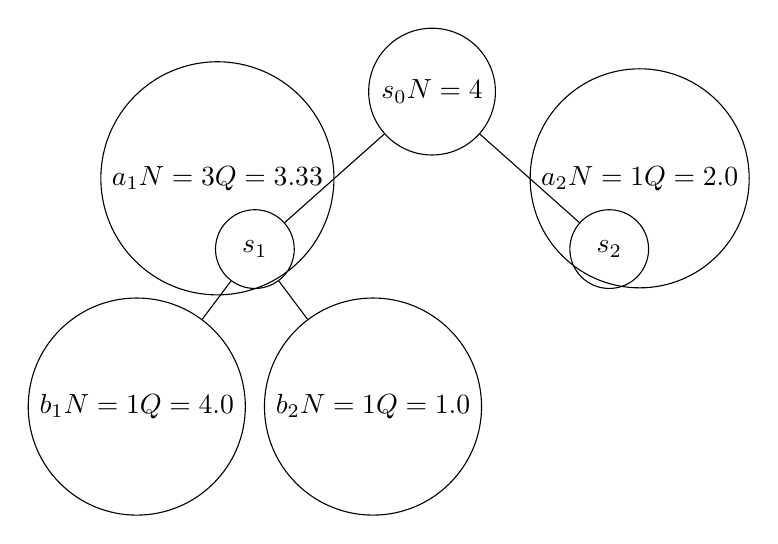
\begin{tikzpicture}[
    level distance=20mm,
    every node/.style={circle,draw,minimum size=10mm},
    level 1/.style={sibling distance=45mm},
    level 2/.style={sibling distance=30mm}
]

\node (s0) {$s_0$\\$N=4$}
    child {
        node {$s_1$}
            child { node {$b_1$\\$N=1$\\$Q=4.0$} }
            child { node {$b_2$\\$N=1$\\$Q=1.0$} }
            edge from parent node[left] {$a_1$\\$N=3$\\$Q=3.33$}
    }
    child {
        node {$s_2$}
            edge from parent node[right] {$a_2$\\$N=1$\\$Q=2.0$}
    };

\end{tikzpicture}


\begin{table}[h!]
\centering
\begin{tabular}{l|l|l}
\textbf{Stopping Rule} & \textbf{Description} & \textbf{Used In} \\
\hline
Terminal State & Stop when episode ends & Board games, deterministic tasks \\
Fixed Horizon & Stop after $N$ rollout steps & Robotics, control \\
Discount Threshold & Stop when rewards become small & Continuous MDPs \\
Heuristic / Value Network & Stop immediately, use $V(s)$ & AlphaZero, MuZero, modern MCTS \\
\end{tabular}
\caption{Summary of stopping criteria used in MCTS simulations.}
\end{table}


\newpage
\pagebreak

% ============================================================
\section*{The MuZero algorithm}

We consider an MDP:
\[
\mathcal{M} = (\mathcal{S}, \mathcal{A}, P, r, \gamma),
\]
where
\[
s_{t+1} \sim P(\cdot \mid s_t, a_t), \qquad 
r_{t+1} = r(s_t,a_t,s_{t+1}),
\]
but MuZero does \emph{not} observe states. It only receives observations
\[
o_t = O(s_t),
\]
where $O$ is unknown.

% ============================================================
\section*{1. MuZero Model Components}

MuZero learns three functions parameterized by $\theta$.

\subsection*{1.1 Representation Function}
Maps observation history to latent state:
\[
s^0 = h_\theta(o_{1:t}).
\]

\subsection*{1.2 Dynamics Function}
Predicts next latent state and reward:
\[
(s^{k+1}, r^k) = g_\theta(s^k, a^k).
\]

\subsection*{1.3 Prediction Function}
Outputs policy logits and value:
\[
(p^k, v^k) = f_\theta(s^k),
\]
where $p^k(a)$ is the prior policy and $v^k$ is the value estimate.

% ============================================================
\section*{2. Latent Rollout (Unrolling the Model)}

Given a real trajectory $(o_{1:t}, a_t, r_{t+1}, a_{t+1}, \dots)$, MuZero builds latent states:

\[
s^0 = h_\theta(o_{1:t}),
\]
\[
(s^{k+1}, \hat{r}^k) = g_\theta(s^k, a_{t+k}),
\]
\[
(p^{k+1}, v^{k+1}) = f_\theta(s^{k+1}),
\qquad k = 0,\dots,K-1.
\]

% ============================================================
\section*{3. MCTS in MuZero (Mathematical)}

MuZero performs tree search entirely in latent space.

\subsection*{3.1 Node Statistics}

For each edge $(s,a)$:
\[
N(s,a) = \text{visit count}, \qquad
W(s,a) = \text{total value}, \qquad
Q(s,a) = \frac{W(s,a)}{N(s,a)}.
\]

Neural network gives prior:
\[
P(s,a) = p(a \mid s).
\]

\subsection*{3.2 PUCT Selection Rule}

MuZero selects:
\[
a^{*} = \arg\max_a \left[ Q(s,a) + U(s,a) \right]
\]
where
\[
U(s,a) 
= c_{\text{puct}} 
\cdot P(s,a) 
\cdot \frac{\sqrt{\sum_b N(s,b)}}{1 + N(s,a)}.
\]

\subsection*{3.3 Expansion}

For first visit of $(s,a)$:
\[
(s', \hat{r}(s,a)) = g_\theta(s,a),
\]
\[
(p(s'), v(s')) = f_\theta(s').
\]

\subsection*{3.4 Value Backup}

At leaf $s^L$, the bootstrap value is:
\[
G = v(s^L).
\]

For each step up the search path:
\[
G \leftarrow r^k + \gamma G,
\]
\[
W(s,a) \leftarrow W(s,a) + G,
\]
\[
N(s,a) \leftarrow N(s,a) + 1,
\]
\[
Q(s,a) = \frac{W(s,a)}{N(s,a)}.
\]

% ============================================================
\section*{4. Training Targets}

\subsection*{4.1 Policy Target}
From root visit counts:
\[
\pi_t(a) = \frac{N(s_t,a)}{\sum_b N(s_t,b)}.
\]

\subsection*{4.2 Value Target (n-step)}
\[
z_t = \sum_{k=0}^{K-1} \gamma^k r_{t+k+1}
+ \gamma^K v(s^{K}).
\]

\subsection*{4.3 Reward Target}
\[
u_{t+k} = r_{t+k+1}.
\]

% ============================================================
\section*{5. MuZero Loss Function}

For unroll steps $k = 0,\dots,K$:

Value loss:
\[
\mathcal{L}_v^k = (v^k - z_{t+k})^2.
\]

Policy loss:
\[
\mathcal{L}_p^k = 
- \sum_{a \in \mathcal{A}} 
\pi_{t+k}(a) \log p^k(a).
\]

Reward loss:
\[
\mathcal{L}_r^k = (r^k - u_{t+k})^2.
\]

Full loss:
\[
\mathcal{L}(\theta)
=
\sum_{k=0}^{K}
\left[
\mathcal{L}_v^k
+
\mathcal{L}_p^k
+
\mathcal{L}_r^k
\right]
+
\lambda \|\theta\|_2^2.
\]

% ============================================================
\section*{6. Complete MuZero Algorithm (Equations)}

\subsection*{6.1 Root Encoding}
\[
s^0 = h_\theta(o_{1:t}).
\]

\subsection*{6.2 Search Iteration}
For each search simulation:

Selection:
\[
a = \arg\max_a 
\left[
Q(s,a) + 
c_{\text{puct}} P(s,a)
\frac{\sqrt{\sum_b N(s,b)}}{1+N(s,a)}
\right].
\]

Expansion:
\[
(s', r) = g_\theta(s,a),
\qquad
(p', v') = f_\theta(s').
\]

Backup:
\[
G = r + \gamma v',
\]
\[
W(s,a) \leftarrow W(s,a) + G,
\qquad
N(s,a) \leftarrow N(s,a) + 1.
\]

\subsection*{6.3 Action Selection}
\[
a_t = \arg\max_a N(s_t,a),
\]
or sample using:
\[
a_t \sim \text{Categorical}(\pi_t).
\]

% ============================================================
\section*{7. Why MuZero Works (Theory)}

MuZero learns a \emph{value-equivalent} model:
\[
v(g_\theta(s,a)) \approx v(P(s,a)),
\]
\[
r(g_\theta(s,a)) \approx r(s,a).
\]

The learned latent states need not satisfy:
\[
s^{k+1} \approx s_{t+k+1},
\]
only:
\[
v(s^{k+1}) \approx v(s_{t+k+1}).
\]

Thus the model is optimized for planning, not reconstruction.

% ============================================================
\section*{8. Summary Pipeline}

\[
o_{1:t}
\overset{h_\theta}{\longrightarrow}
s^0
\overset{\text{MCTS}}{\longrightarrow}
\pi_t
\]

\[
(s^{k+1}, r^k) = g_\theta(s^k, a_{t+k}),
\]
\[
(p^k, v^k) = f_\theta(s^k),
\]

\[
z_t = r_t + \gamma r_{t+1} + \dots + \gamma^K v^{K},
\]

\[
\mathcal{L} = \sum_k (v^k - z_{t+k})^2
- \sum_a \pi_{t+k}(a)\log p^k(a)
+ (r^k - u_{t+k})^2
+ \lambda\|\theta\|^2.
\]

\newpage
\pagebreak



\newpage
\pagebreak

\section*{Constrained Markov Decision Process (CMDP) and Lagrangian PPO}

%%%%%%%%%%%%%%%%%%%%%%%%%%%%%%%%%%%%%%%%%%%%%%%%%%%%%%%%%%%%%%
\subsection*{1. CMDP Definition}

A \textbf{Constrained Markov Decision Process (CMDP)} is defined as:
\[
\mathcal{M}_{\text{CMDP}}
=
\langle
\mathcal{S},
\mathcal{A},
P,
r,
\{c^{(k)}\}_{k=1}^K,
\gamma
\rangle
\]
where:
\[
\begin{aligned}
&s_t \in \mathcal{S} &&\text{state at time } t \\
&a_t \in \mathcal{A} &&\text{action at time } t \\
&P(s_{t+1}\mid s_t,a_t) &&\text{transition kernel} \\
&r(s_t,a_t) &&\text{reward function} \\
&c^{(k)}(s_t,a_t) &&\text{cost function for constraint } k \\
&\gamma \in (0,1) &&\text{discount factor}
\end{aligned}
\]

%%%%%%%%%%%%%%%%%%%%%%%%%%%%%%%%%%%%%%%%%%%%%%%%%%%%%%%%%%%%%%
\subsection*{2. Objective and Constraints}

The CMDP objective is:
\[
\max_{\pi}
\;
J_R(\pi)
=
\mathbb{E}_\pi
\left[
\sum_{t=0}^{\infty}
\gamma^t r(s_t,a_t)
\right]
\]

subject to expected discounted cost constraints:
\[
J_{C_k}(\pi)
=
\mathbb{E}_\pi
\left[
\sum_{t=0}^{\infty}
\gamma^t c^{(k)}(s_t,a_t)
\right]
\;\le\;
d_k,
\qquad
k=1,\dots,K
\]

where K is the total number of constraints. $d_k \in \mathbb{R}_{\ge 0}$ denotes the maximum allowable expected discounted cost for constraint 
\(k\). $J_{C_k}(\pi)$ is the long-term expected cost under policy .

%%%%%%%%%%%%%%%%%%%%%%%%%%%%%%%%%%%%%%%%%%%%%%%%%%%%%%%%%%%%%%
\subsection*{3. Lagrangian Relaxation}

Introduce non-negative Lagrange multipliers:
\[
\lambda_k \ge 0
\]

The Lagrangian objective is:
\[
\mathcal{L}(\pi,\lambda)
=
J_R(\pi)
-
\sum_{k=1}^K
\lambda_k
\left(
J_{C_k}(\pi) - d_k
\right)
\].


\paragraph{Why Lagrangian Uses $\lambda_k$}
Each constraint in a CMDP is enforced using its own non-negative Lagrange multiplier \( \lambda_k \ge 0 \). The Lagrangian objective is:
\[
\mathcal{L}(\pi,\lambda)
=
J_R(\pi)
-
\sum_{k=1}^{K}
\lambda_k
\left(
J_{C_k}(\pi) - d_k
\right).
\]

If constraint \( k \) is violated, i.e.,
\[
J_{C_k}(\pi) > d_k,
\]
then the corresponding multiplier increases:
\[
\lambda_k \uparrow.
\]

If constraint \( k \) is satisfied, i.e.,
\[
J_{C_k}(\pi) \le d_k,
\]
then the corresponding multiplier decreases:
\[
\lambda_k \downarrow.
\]

This iterative adjustment of \( \lambda_k \) via gradient ascent on the dual variables is known as \textbf{dual ascent}. The constrained problem becomes a saddle-point problem:
\[
\max_{\pi}
\min_{\lambda \ge 0}
\;
\mathcal{L}(\pi,\lambda)
\]


\begin{mdframed}[linecolor=red, linewidth=2pt]
\section*{Understanding the Saddle-Point Formulation in CMDPs}

This section provides a detailed, first-principles explanation of the saddle-point formulation
\[
\max_{\pi}\;\min_{\lambda \ge 0}\; \mathcal{L}(\pi,\lambda)
\]
which lies at the core of Constrained Markov Decision Processes (CMDPs).

%%%%%%%%%%%%%%%%%%%%%%%%%%%%%%%%%%%%%%%%%%%%%%%%%%%%%%%%%%%%%%
\subsection*{1. What Problem Are We Solving?}

In a CMDP, the goal is not merely to maximize reward, but to do so while respecting
safety, budget, or resource constraints. The original constrained optimization problem is:

\[
\begin{aligned}
\max_{\pi} \quad
& J_R(\pi) \\
\text{s.t.} \quad
& J_{C_k}(\pi) \le d_k,
\quad k = 1,\dots,K
\end{aligned}
\]

This formulation means:

\begin{quote}
Among all policies that satisfy the constraints, choose the one with the highest reward.
\end{quote}

Directly optimizing this problem is difficult because constraints depend on long-term
expectations and policies are typically parameterized by neural networks.

%%%%%%%%%%%%%%%%%%%%%%%%%%%%%%%%%%%%%%%%%%%%%%%%%%%%%%%%%%%%%%
\subsection*{2. The Lagrangian Reformulation}

To handle constraints, we introduce non-negative Lagrange multipliers
\( \lambda_k \ge 0 \) and define the \emph{Lagrangian}:

\[
\boxed{
\mathcal{L}(\pi,\lambda)
=
J_R(\pi)
-
\sum_{k=1}^K
\lambda_k
\bigl(
J_{C_k}(\pi) - d_k
\bigr)
}
\]

Each term has a clear interpretation:
\begin{itemize}
    \item \( J_R(\pi) \): the expected return to be maximized,
    \item \( J_{C_k}(\pi) - d_k \): the violation of constraint \(k\),
    \item \( \lambda_k \): the strength of the penalty for violating constraint \(k\).
\end{itemize}

The Lagrangian is a single scalar objective that trades off reward against constraint violations.

%%%%%%%%%%%%%%%%%%%%%%%%%%%%%%%%%%%%%%%%%%%%%%%%%%%%%%%%%%%%%%
\subsection*{3. Why Minimize Over \( \lambda \ge 0 \)?}

For a fixed policy \( \pi \), we consider the inner problem:
\[
\min_{\lambda \ge 0} \mathcal{L}(\pi,\lambda).
\]

This means: given a policy, allow the multipliers to apply the strongest possible penalty.

\paragraph{Case 1: Policy Satisfies All Constraints}

If
\[
J_{C_k}(\pi) \le d_k \quad \forall k,
\]
then
\[
J_{C_k}(\pi) - d_k \le 0.
\]

The penalty term becomes:
\[
-\lambda_k (J_{C_k}(\pi) - d_k)
=
\lambda_k (d_k - J_{C_k}(\pi)) \ge 0.
\]

Increasing \( \lambda_k \) increases the Lagrangian, so the minimizing choice is:
\[
\lambda_k^* = 0.
\]

Thus,
\[
\min_{\lambda \ge 0} \mathcal{L}(\pi,\lambda)
=
J_R(\pi).
\]

Feasible policies incur no penalty.

\paragraph{Case 2: Policy Violates a Constraint}

If for some \( k \),
\[
J_{C_k}(\pi) > d_k,
\]
then
\[
J_{C_k}(\pi) - d_k > 0.
\]

Now the penalty term is negative, and as \( \lambda_k \to \infty \),
\[
\mathcal{L}(\pi,\lambda) \to -\infty.
\]

Therefore,
\[
\min_{\lambda \ge 0} \mathcal{L}(\pi,\lambda) = -\infty.
\]

Any infeasible policy is thus eliminated.

%%%%%%%%%%%%%%%%%%%%%%%%%%%%%%%%%%%%%%%%%%%%%%%%%%%%%%%%%%%%%%
\subsection*{4. Effect of the Inner Minimization}

After minimizing over \( \lambda \), the Lagrangian evaluates to:
\[
\min_{\lambda \ge 0} \mathcal{L}(\pi,\lambda)
=
\begin{cases}
J_R(\pi), & \pi \text{ satisfies all constraints}, \\
-\infty, & \pi \text{ violates any constraint}.
\end{cases}
\]

The inner minimization acts as an exact feasibility filter.

%%%%%%%%%%%%%%%%%%%%%%%%%%%%%%%%%%%%%%%%%%%%%%%%%%%%%%%%%%%%%%
\subsection*{5. Why Maximize Over \( \pi \)?}

Applying the outer maximization,
\[
\max_{\pi} \min_{\lambda \ge 0} \mathcal{L}(\pi,\lambda),
\]
automatically discards infeasible policies and yields:
\[
\max_{\pi \in \text{feasible}} J_R(\pi),
\]
which is exactly the original CMDP objective.

%%%%%%%%%%%%%%%%%%%%%%%%%%%%%%%%%%%%%%%%%%%%%%%%%%%%%%%%%%%%%%
\subsection*{6. Why This Is a Saddle-Point Problem}

A pair \( (\pi^*, \lambda^*) \) is a saddle point if:
\[
\mathcal{L}(\pi,\lambda^*)
\;\le\;
\mathcal{L}(\pi^*,\lambda^*)
\;\le\;
\mathcal{L}(\pi^*,\lambda).
\]

This implies:
\begin{itemize}
    \item the policy \( \pi^* \) cannot improve reward without violating constraints,
    \item the multipliers \( \lambda^* \) cannot further penalize the solution,
    \item neither player can improve unilaterally.
\end{itemize}

This can be viewed as a two-player zero-sum game:

\begin{center}
\begin{tabular}{|c|c|c|}
\hline
Player & Variable & Objective \\
\hline
Primal & Policy \( \pi \) & Maximize reward \\
Dual & Multipliers \( \lambda \) & Enforce constraints \\
\hline
\end{tabular}
\end{center}

%%%%%%%%%%%%%%%%%%%%%%%%%%%%%%%%%%%%%%%%%%%%%%%%%%%%%%%%%%%%%%
\subsection*{7. Algorithmic Interpretation}

In practical algorithms such as Lagrangian PPO, the saddle-point problem is solved
via alternating updates:

\begin{itemize}
    \item \textbf{Policy update (gradient ascent):}
    \[
    \theta \leftarrow \theta + \alpha \nabla_\theta \mathcal{L}(\pi_\theta,\lambda)
    \]
    \item \textbf{Multiplier update (projected gradient descent):}
    \[
    \lambda_k \leftarrow \bigl[\lambda_k + \eta(J_{C_k}(\pi) - d_k)\bigr]_+
    \]
\end{itemize}

This procedure is known as \emph{primal--dual optimization}.

%%%%%%%%%%%%%%%%%%%%%%%%%%%%%%%%%%%%%%%%%%%%%%%%%%%%%%%%%%%%%%
\subsection*{8. One-Sentence Intuition}

\begin{quote}
The saddle-point formulation guarantees that any policy violating constraints is penalized
infinitely by the dual variables, so maximizing the minimum Lagrangian recovers exactly the
optimal feasible policy.
\end{quote}

\end{mdframed}



%%%%%%%%%%%%%%%%%%%%%%%%%%%%%%%%%%%%%%%%%%%%%%%%%%%%%%%%%%%%%%
\subsection*{4. Augmented Reward and Lagrangian Objective}

Recall the CMDP objective:
\[
\max_{\pi}
\; J_R(\pi)
\quad
\text{s.t.}
\quad
J_{C_k}(\pi) \le d_k,
\qquad k=1,\dots,K,
\]
where
\[
\begin{aligned}
J_R(\pi)
&=
\mathbb{E}_\pi
\left[
\sum_{t=0}^{\infty}
\gamma^t r(s_t,a_t)
\right], \\
J_{C_k}(\pi)
&=
\mathbb{E}_\pi
\left[
\sum_{t=0}^{\infty}
\gamma^t c^{(k)}(s_t,a_t)
\right].
\end{aligned}
\]

Introduce non-negative Lagrange multipliers \( \lambda_k \ge 0 \) and form the Lagrangian:
\[
\mathcal{L}(\pi,\lambda)
=
J_R(\pi)
-
\sum_{k=1}^K
\lambda_k
\left(
J_{C_k}(\pi) - d_k
\right).
\]

Define the \emph{augmented (Lagrangian) reward}:
\[
\tilde{r}_\lambda(s,a)
=
r(s,a)
-
\sum_{k=1}^K
\lambda_k c^{(k)}(s,a).
\]

Then the Lagrangian can be rewritten as:
\[
\begin{aligned}
\mathcal{L}(\pi,\lambda)
&=
\mathbb{E}_\pi
\left[
\sum_{t=0}^{\infty}
\gamma^t
\tilde{r}_\lambda(s_t,a_t)
\right]
+
\sum_{k=1}^K
\lambda_k d_k.
\end{aligned}
\]

The term \( \sum_k \lambda_k d_k \) is constant with respect to \( \pi \) and therefore does not affect the policy gradient.

%%%%%%%%%%%%%%%%%%%%%%%%%%%%%%%%%%%%%%%%%%%%%%%%%%%%%%%%%%%%%%
\subsection*{5. Lagrangian Value, Action-Value, and Advantage Functions}
For a fixed multiplier vector \( \lambda \), define the Lagrangian value
functions under policy \( \pi \). State-value function:
\[
V_\lambda^\pi(s)
=
\mathbb{E}_\pi
\left[
\sum_{t=0}^{\infty}
\gamma^t
\tilde{r}_\lambda(s_t,a_t)
\;\middle|\;
s_0 = s
\right].
\]

Action-value function:
\[
\begin{aligned}
Q_\lambda^\pi(s,a)
&=
\tilde{r}_\lambda(s,a)
+
\gamma
\mathbb{E}_{s'\sim P(\cdot|s,a)}
\left[
V_\lambda^\pi(s')
\right].
\end{aligned}
\]

The corresponding Lagrangian advantage is:
\[
A_\lambda^\pi(s,a)
=
Q_\lambda^\pi(s,a)
-
V_\lambda^\pi(s).
\]

%%%%%%%%%%%%%%%%%%%%%%%%%%%%%%%%%%%%%%%%%%%%%%%%%%%%%%%%%%%%%%
\subsection*{6. Lagrangian Policy Gradient}
Let \( \pi_\theta(a|s) \) be a differentiable stochastic policy.
For fixed \( \lambda \), the gradient of the Lagrangian with respect to
policy parameters \( \theta \) is given by the policy gradient theorem:

\[
\begin{aligned}
\nabla_\theta \mathcal{L}(\pi_\theta,\lambda)
&=
\nabla_\theta
\mathbb{E}_{\pi_\theta}
\left[
\sum_{t=0}^{\infty}
\gamma^t
\tilde{r}_\lambda(s_t,a_t)
\right] \\
&=
\mathbb{E}_{\pi_\theta}
\left[
\sum_{t=0}^{\infty}
\gamma^t
\nabla_\theta
\log \pi_\theta(a_t|s_t)
\;
A_\lambda^\pi(s_t,a_t)
\right].
\end{aligned}
\]

Thus, from the perspective of the policy update, the CMDP reduces to an
unconstrained MDP with reward \( \tilde{r}_\lambda \).

%%%%%%%%%%%%%%%%%%%%%%%%%%%%%%%%%%%%%%%%%%%%%%%%%%%%%%%%%%%%%%
\subsection*{7. Lagrangian PPO Objective (Primal Update)}

Let \( \pi_{\theta_{\text{old}}} \) denote the behavior policy used to collect
data. Define the importance sampling ratio:
\[
r_t(\theta)
=
\frac{\pi_\theta(a_t|s_t)}
{\pi_{\theta_{\text{old}}}(a_t|s_t)}.
\]

In practice, the Lagrangian advantage is constructed by combining reward and
cost advantages:
\[
A_{\lambda,t}
=
A_R(s_t,a_t)
-
\sum_{k=1}^K
\lambda_k
A_{C_k}(s_t,a_t).
\]

The clipped PPO surrogate objective for the \emph{primal} optimization problem
is:
\[
\mathcal{J}_{\text{PPO}}(\theta;\lambda)
=
\mathbb{E}
\left[
\min
\left(
r_t(\theta)\,A_{\lambda,t},
\;
\text{clip}
\big(r_t(\theta),1-\epsilon,1+\epsilon\big)
A_{\lambda,t}
\right)
\right].
\]

This objective is maximized with respect to \( \theta \) while holding
\( \lambda \) fixed.

%%%%%%%%%%%%%%%%%%%%%%%%%%%%%%%%%%%%%%%%%%%%%%%%%%%%%%%%%%%%%%
\subsection*{8. Reward and Cost Critics}

Separate critics are maintained for the reward and each cost.

Reward value function:
\[
V_R^\pi(s)
=
\mathbb{E}_\pi
\left[
\sum_{t=0}^{\infty}
\gamma^t r(s_t,a_t)
\;\middle|\;
s_0=s
\right].
\]

Cost value functions:
\[
V_{C_k}^\pi(s)
=
\mathbb{E}_\pi
\left[
\sum_{t=0}^{\infty}
\gamma^t c^{(k)}(s_t,a_t)
\;\middle|\;
s_0=s
\right].
\]

Define temporal-difference residuals:
\[
\begin{aligned}
\delta_{R,t}
&=
r_t
+
\gamma V_R(s_{t+1})
-
V_R(s_t), \\
\delta_{C_k,t}
&=
c_t^{(k)}
+
\gamma V_{C_k}(s_{t+1})
-
V_{C_k}(s_t).
\end{aligned}
\]

Generalized Advantage Estimation (GAE) is applied separately:
\[
\begin{aligned}
A_R^{\text{GAE}}(t)
&=
\sum_{l=0}^{\infty}
(\gamma\lambda_{\text{GAE}})^l
\delta_{R,t+l}, \\
A_{C_k}^{\text{GAE}}(t)
&=
\sum_{l=0}^{\infty}
(\gamma\lambda_{\text{GAE}})^l
\delta_{C_k,t+l}.
\end{aligned}
\]

%%%%%%%%%%%%%%%%%%%%%%%%%%%%%%%%%%%%%%%%%%%%%%%%%%%%%%%%%%%%%%
\subsection*{9. Dual Variable Update (Constraint Enforcement)}

Hold $\theta$ fixed (i.e., fixed $\pi_\theta$). Consider the dependence of
$\mathcal{L}$ on $\lambda_k$:

\[
\mathcal{L}(\theta,\lambda)
=
J_R(\pi_\theta)
-
\sum_{j=1}^{K}
\lambda_j
\big(
J_{C_j}(\pi_\theta)
-
d_j
\big).
\]

For a particular $k$, the only term depending on $\lambda_k$ is
\[
-
\lambda_k
\big(
J_{C_k}(\pi_\theta)
-
d_k
\big).
\]

Thus:
\[
\frac{\partial \mathcal{L}}{\partial \lambda_k}
=
-
\big(
J_{C_k}(\pi_\theta)
-
d_k
\big)
=
d_k
-
J_{C_k}(\pi_\theta).
\]

This matches exactly what you wrote.

\paragraph{Interpretation of the sign}

If the constraint is violated,
\[
J_{C_k}(\pi_\theta) > d_k,
\]
then
\[
\frac{\partial \mathcal{L}}{\partial \lambda_k}
=
d_k
-
J_{C_k}(\pi_\theta)
<
0,
\]
meaning increasing $\lambda_k$ decreases $\mathcal{L}$ (stronger penalty).
In the dual problem, we want to increase $\lambda_k$ when violated, which is
why the dual update is a descent step on the dual objective, or equivalently
an ascent step on the constraint violation term. Dual ascent is therefore performed as:
\[
\lambda_k
\leftarrow
\Big[
\lambda_k
+
\eta_\lambda
\big(
J_{C_k}(\pi_\theta)
-
d_k
\big)
\Big]_+,
\]
where $[\cdot]_+ \triangleq \max(\cdot,0)$ denotes projection onto the
nonnegative orthant, enforcing the dual feasibility constraint
$\lambda_k \ge 0$.  Formally, for any real number $x \in \mathbb{R}$,
\[
[x]_+ \;\triangleq\; \max(x,0).
\]

That is:
\[
\text{if } x \ge 0,\ \text{then } [x]_+ = x,
\]
\[
\text{if } x < 0,\ \text{then } [x]_+ = 0(Clipped to zero).
\]

%%%%%%%%%%%%%%%%%%%%%%%%%%%%%%%%%%%%%%%%%%%%%%%%%%%%%%%%%%%%%%
\subsection*{11. Final Primal--Dual Optimization Loop}

\[
\boxed{
\begin{aligned}
\textbf{Primal step:}\quad
& \theta
\leftarrow
\arg\max_\theta
\;
\mathcal{J}_{\text{PPO}}(\theta;\lambda), \\[6pt]
\textbf{Dual step:}\quad
& \lambda_k
\leftarrow
\Big[
\lambda_k
+
\eta_\lambda
\big(
J_{C_k}(\pi_\theta) - d_k
\big)
\Big]_+.
\end{aligned}
}
\]


\begin{mdframed}
    %%%%%%%%%%%%%%%%%%%%%%%%%%%%%%%%%%%%%%%%%%%%%%%%%%%%%%%%%%%%%%
\subsection*{Neural Networks in Lagrangian PPO (CMDP)}

We explicitly identify all neural networks used in Lagrangian PPO and clarify
their outputs and roles in the optimization.

%%%%%%%%%%%%%%%%%%%%%%%%%%%%%%%%%%%%%%%%%%%%%%%%%%%%%%%%%%%%%%
\subsection*{1. Actor Network (Policy)}

The actor is a stochastic policy parameterized by \( \theta \):
\[
\pi_\theta(a \mid s).
\]

\paragraph{Parameters.}
\[
\theta \quad \text{(trainable via PPO)}.
\]

\paragraph{Outputs.}
\begin{itemize}
    \item \textbf{Discrete action space:}
    \[
    \pi_\theta(a \mid s)
    =
    \text{Softmax}(f_\theta(s)),
    \]
    which outputs a probability distribution over actions.

    \item \textbf{Continuous action space:}
    \[
    \pi_\theta(a \mid s)
    =
    \mathcal{N}
    \big(
    \mu_\theta(s),\;
    \Sigma_\theta(s)
    \big),
    \]
    which outputs a mean vector \( \mu_\theta(s) \) and (diagonal) covariance
    \( \Sigma_\theta(s) \).
\end{itemize}

\paragraph{Where it appears in the equations.}
\begin{enumerate}
    \item Importance sampling ratio:
    \[
    r_t(\theta)
    =
    \frac{\pi_\theta(a_t \mid s_t)}
    {\pi_{\theta_{\text{old}}}(a_t \mid s_t)}.
    \]

    \item Policy gradient term:
    \[
    \nabla_\theta
    \log \pi_\theta(a_t \mid s_t).
    \]

    \item PPO surrogate objective:
    \[
    \mathcal{J}_{\text{PPO}}(\theta;\lambda)
    =
    \mathbb{E}
    \left[
    \min
    \left(
    r_t(\theta) A_{\lambda,t},
    \;
    \text{clip}(r_t(\theta),1-\epsilon,1+\epsilon) A_{\lambda,t}
    \right)
    \right].
    \]
\end{enumerate}

%%%%%%%%%%%%%%%%%%%%%%%%%%%%%%%%%%%%%%%%%%%%%%%%%%%%%%%%%%%%%%
\subsection*{2. Reward Critic Network}

The reward critic estimates the discounted return under policy \( \pi \):
\[
V_{R,\psi_R}(s).
\]

\paragraph{Parameters.}
\[
\psi_R \quad \text{(trainable)}.
\]

\paragraph{Output.}
\[
V_R^\pi(s)
\approx
\mathbb{E}_\pi
\left[
\sum_{t=0}^{\infty}
\gamma^t r_t
\right].
\]

\paragraph{Where it appears.}
\begin{enumerate}
    \item Reward TD residual:
    \[
    \delta_{R,t}
    =
    r_t
    +
    \gamma V_{R,\psi_R}(s_{t+1})
    -
    V_{R,\psi_R}(s_t).
    \]

    \item Reward GAE:
    \[
    A_R^{\text{GAE}}(t)
    =
    \sum_{l=0}^{\infty}
    (\gamma\lambda_{\text{GAE}})^l
    \delta_{R,t+l}.
    \]
\end{enumerate}

%%%%%%%%%%%%%%%%%%%%%%%%%%%%%%%%%%%%%%%%%%%%%%%%%%%%%%%%%%%%%%
\subsection*{3. Cost Critic Networks (One per Constraint)}

For each constraint \( k = 1,\dots,K \), a separate cost critic is used:
\[
V_{C_k,\psi_{C_k}}(s).
\]

\paragraph{Parameters.}
\[
\psi_{C_k} \quad \text{(trainable)}.
\]

\paragraph{Output.}
\[
V_{C_k}^\pi(s)
\approx
\mathbb{E}_\pi
\left[
\sum_{t=0}^{\infty}
\gamma^t c_t^{(k)}
\right].
\]

\paragraph{Where they appear.}
\begin{enumerate}
    \item Cost TD residual:
    \[
    \delta_{C_k,t}
    =
    c_t^{(k)}
    +
    \gamma V_{C_k,\psi_{C_k}}(s_{t+1})
    -
    V_{C_k,\psi_{C_k}}(s_t).
    \]

    \item Cost GAE:
    \[
    A_{C_k}^{\text{GAE}}(t)
    =
    \sum_{l=0}^{\infty}
    (\gamma\lambda_{\text{GAE}})^l
    \delta_{C_k,t+l}.
    \]
\end{enumerate}

%%%%%%%%%%%%%%%%%%%%%%%%%%%%%%%%%%%%%%%%%%%%%%%%%%%%%%%%%%%%%%
\subsection*{4. Lagrangian Advantage (No Neural Network)}

The Lagrangian advantage is computed algebraically as:
\[
A_{\lambda,t}
=
A_R^{\text{GAE}}(t)
-
\sum_{k=1}^K
\lambda_k
A_{C_k}^{\text{GAE}}(t).
\]

No neural network directly outputs \( A_{\lambda,t} \); it is formed by a linear
combination of critic-based advantages.

%%%%%%%%%%%%%%%%%%%%%%%%%%%%%%%%%%%%%%%%%%%%%%%%%%%%%%%%%%%%%%
\subsection*{5. Dual Variables (Not Neural Networks)}

The Lagrange multipliers are scalar variables:
\[
\lambda_k \ge 0.
\]

They are not produced by neural networks and are updated via projected
gradient ascent:
\[
\lambda_k
\leftarrow
\Big[
\lambda_k
+
\eta_\lambda
\big(
J_{C_k}(\pi) - d_k
\big)
\Big]_+.
\]

\end{mdframed}


\newpage
\pagebreak


\section*{Decision Transformer}

\subsection*{Reinforcement Learning as Conditional Sequence Modeling}

\hrulefill

\section*{1. Offline Reinforcement Learning Setting}

We consider an offline reinforcement learning problem defined over a Markov Decision Process (MDP)
\[
\mathcal{M} = (\mathcal{S}, \mathcal{A}, P, r),
\]
where $\mathcal{S}$ is the state space, $\mathcal{A}$ is the action space,
$P(s_{t+1}\mid s_t,a_t)$ is the transition kernel, and
$r(s_t,a_t)$ is the reward function.

We are given a fixed dataset of trajectories collected by an unknown behavior policy:
\[
\mathcal{D}
=
\left\{
\tau^{(i)}
=
\big(
s^{(i)}_0,a^{(i)}_0,r^{(i)}_0;\;
s^{(i)}_1,a^{(i)}_1,r^{(i)}_1;\;
\dots;\;
s^{(i)}_{T_i}
\big)
\right\}_{i=1}^{N}.
\]

Rewards are defined as
\[
r^{(i)}_t = r\!\left(s^{(i)}_t,a^{(i)}_t\right),
\qquad
t = 0,\dots,T_i-1.
\]

The terminal state $s_{T_i}$ has no associated action or reward.
No interaction with the environment is allowed during training.

\hrulefill

\section*{2. Return-to-Go (RTG)}

For each trajectory $\tau^{(i)}$, define the return-to-go at timestep $t$ as
\[
R^{(i)}_t
=
\sum_{k=t}^{T_i-1} r^{(i)}_k.
\]

Return-to-go is a conditioning variable, not a prediction target.

Each trajectory is relabeled as
\[
\tau^{(i)}
=
(R^{(i)}_0,s^{(i)}_0,a^{(i)}_0;\;
R^{(i)}_1,s^{(i)}_1,a^{(i)}_1;\;
\dots;\;
R^{(i)}_{T_i},s^{(i)}_{T_i}).
\]

\hrulefill

\section*{3. Probabilistic Modeling Objective}

Decision Transformer models the conditional distribution over action sequences
\[
p_\theta(a_{0:T_i-1} \mid R_{0:T_i}, s_{0:T_i}).
\]

Using causal factorization, this distribution is written as
\[
p_\theta(a_{0:T_i-1} \mid \cdot)
=
\prod_{t=0}^{T_i-1}
p_\theta\!\left(
a_t
\mid
R_{\le t},\;
s_{\le t},\;
a_{<t}
\right).
\]

No value function, $Q$-function, Bellman backup, or environment model is learned.

\hrulefill

\section*{4. Tokenization of Experience}

Each environment timestep $t$ produces three semantic tokens:
\[
x_{t,1} = R_t,
\qquad
x_{t,2} = s_t,
\qquad
x_{t,3} = a_t.
\]

During training, $a_t$ is observed (teacher forcing).
During inference, $a_t$ is predicted autoregressively.

\hrulefill

\section*{5. Fixed Context Window}

Decision Transformer uses a fixed context length $K$, corresponding to the
number of \emph{past} timesteps included in the model input.

At decision time $t$, define
\[
t' = \max(0, t-K).
\]

The input sequence consists of:
\[
(R_{t'}, s_{t'}, a_{t'};\;
\dots;\;
R_{t-1}, s_{t-1}, a_{t-1};\;
R_t, s_t).
\]

That is, all tokens $(R_\tau, s_\tau, a_\tau)$ for $\tau = t',\dots,t-1$
are included, along with $(R_t, s_t)$ from the current timestep.
The action $a_t$ is excluded and must be predicted.

Under this convention, the total number of tokens is
\[
L = 3K + 1.
\]

This yields $\mathcal{O}(K^2)$ attention complexity per decision step.

\hrulefill

\section*{6. Token Embedding Functions}

Let $d_{\text{model}}$ denote the Transformer hidden dimension.
Each raw token value is mapped to $\mathbb{R}^{d_{\text{model}}}$ via
a content embedding function:
\[
\begin{aligned}
e(R_t) &= W_R R_t + b_R, \\
e(s_t) &= f_S(s_t), \\
e(a_t) &= f_A(a_t),
\end{aligned}
\qquad
e(\cdot)\in\mathbb{R}^{d_{\text{model}}}.
\]

The content embedding encodes \emph{what} the token represents, but does
not encode temporal information.

\hrulefill

\section*{7. Temporal (Timestep) Embeddings}

In Decision Transformer, multiple tokens originate from the same
environment timestep.
To explicitly encode this structure, temporal (timestep) embeddings are used.

Let
\[
\phi : \mathbb{N} \rightarrow \mathbb{R}^{d_{\text{model}}}
\]
be a learnable embedding function that maps an environment timestep $t$
to a vector.

Each token $x_i$ in the flattened input sequence is associated with an
environment timestep via a mapping $\tau(i)$, defined such that
$\tau(i)=t$ if token $x_i$ was generated at timestep $t$.

The final token representation is
\[
z_i = e(x_i) + \phi\!\left(\tau(i)\right).
\]

As a result, all tokens $(R_t, s_t, a_t)$ corresponding to the same
environment timestep share the same temporal embedding $\phi(t)$.
This explicitly informs the Transformer that these tokens occurred
simultaneously in the environment.

\hrulefill

\section*{8. Transformer Architecture}

Let
\[
Z^{(0)} = [z_1,\dots,z_L] \in \mathbb{R}^{L \times d_{\text{model}}}.
\]

A decoder-only Transformer with $N$ layers is applied.
For layer $\ell$:

\paragraph{Pre-layer normalization}
\[
X = \mathrm{LN}(Z^{(\ell-1)}).
\]

\paragraph{Self-attention}
\[
Q = XW_Q,
\qquad
K = XW_K,
\qquad
V = XW_V.
\]

\[
\mathrm{Attn}(X)
=
\mathrm{softmax}
\!\left(
\frac{QK^\top}{\sqrt{d_k}} + M
\right)V,
\]
with causal mask
\[
M_{ij} =
\begin{cases}
0, & j \le i, \\
-\infty, & j > i.
\end{cases}
\]

\paragraph{Residual update}
\[
Z^{(\ell)} =
Z^{(\ell-1)} +
\mathrm{Attn}(X) +
\mathrm{FFN}(\cdot).
\]

This enforces causal conditioning.

\hrulefill

\section*{9. Transformer Outputs and Alignment}

Let
\[
H = [h_1,\dots,h_L]
\]
denote the final hidden states.

For a given timestep $t$, only the hidden state corresponding to the
state token $s_t$ is used for action prediction:
\[
\begin{aligned}
h(R_t) &\text{ is ignored}, \\
h(s_t) &\rightarrow a_t \quad \text{(used)}, \\
h(a_t) &\text{ is ignored}.
\end{aligned}
\]

No loss is applied to predictions from $h(R_t)$ or $h(a_t)$.

\hrulefill

\section*{10. Action Prediction Head}

\subsection*{Continuous Action Space (Original Paper)}

Decision Transformer is deterministic:
\[
\hat{a}_t = g_\theta\!\left(h(s_t)\right),
\]
optionally followed by $\tanh$ to enforce action bounds.

\subsection*{Discrete Action Space}

\[
\pi_\theta(a_t \mid \cdot)
=
\mathrm{softmax}\!\left(W h(s_t)\right).
\]

\hrulefill

\section*{11. Training Objective}

\subsection*{Continuous Control}

\[
\min_\theta
\;
\mathbb{E}_{\tau \sim \mathcal{D}}
\left[
\sum_{t=0}^{T_i-1}
\left\|
a_t - \hat{a}_t
\right\|_2^2
\right].
\]

\subsection*{Discrete Control}

\[
\min_\theta
\;
-
\mathbb{E}_{\tau \sim \mathcal{D}}
\left[
\sum_{t}
\log
p_\theta(a_t \mid R_{\le t}, s_{\le t}, a_{<t})
\right].
\]

No auxiliary losses are used.

\hrulefill

\section*{12. What Decision Transformer Is Not}

Decision Transformer does not:
\begin{itemize}
\item learn a reward model,
\item learn a transition model,
\item learn a value or $Q$ function,
\item perform planning or search,
\item apply Bellman updates.
\end{itemize}

It performs maximum-likelihood estimation of actions conditioned on returns.

\hrulefill

\section*{13. Final Theoretical Statement}

\[
\boxed{
\text{Decision Transformer is a causal sequence model that directly learns}
}
\]
\[
\boxed{
p(a_t \mid R_{\le t}, s_{\le t}, a_{<t})
\text{ via supervised learning, without value functions.}
}
\]

\newpage
\clearpage


\hrulefill

\section*{GRPO}

We assume:

\begin{itemize}
    \item an SLM $(\pi_\theta)$ (typically 0.5B--3B),
    \item fine-tuned using \textbf{GRPO}, possibly with \textbf{KL anchoring}, \textbf{QLoRA}, and \textbf{verifier rewards},
    \item \textbf{no value function}, \textbf{no critic}, \textbf{no TD learning}.
\end{itemize}

\hrulefill

\section*{1. Core Objects and Notation (Fixed)}

\begin{itemize}
    \item Prompt: $x \in \mathcal{X}$
    \item Sampled responses (group):
    \[
    \mathcal{G}(x) = \{ y^{(1)}, \dots, y^{(K)} \}
    \]
    \item Policy (autoregressive):
    \[
    \pi_\theta(y \mid x)
    =
    \prod_{t=1}^{T}
    \pi_\theta(y_t \mid x, y_{<t})
    \]
    \item Reward (scalar, sequence-level):
    \[
    R_i = R(x, y^{(i)})
    \]
\end{itemize}

\hrulefill

\section*{2. Group-Relative Advantage (No Critic)}

Compute group mean reward:
\[
\bar{R}_{\mathcal{G}}
=
\frac{1}{K}
\sum_{j=1}^{K} R_j
\]

Group-relative advantage:
\[
\boxed{
A_i = R_i - \bar{R}_{\mathcal{G}}
}
\]

Key property:
\[
\sum_{i=1}^{K} A_i = 0
\]

This replaces \textbf{value-function baselines} entirely.

\hrulefill

\section*{3. Policy Likelihood Ratio (PPO-Compatible)}

Let $\theta_{\text{old}}$ be the frozen sampling policy.

Sequence-level likelihood ratio:
\[
r_\theta(y^{(i)} \mid x)
=
\frac{
\pi_\theta(y^{(i)} \mid x)
}{
\pi_{\theta_{\text{old}}}(y^{(i)} \mid x)
}
\]

Expanded:
\[
\log r_\theta(y^{(i)} \mid x)
=
\sum_{t=1}^{T_i}
\log
\frac{
\pi_\theta(y_t^{(i)} \mid x, y_{<t}^{(i)})
}{
\pi_{\theta_{\text{old}}}(y_t^{(i)} \mid x, y_{<t}^{(i)})
}
\]

\hrulefill

\section*{4. Primary GRPO Loss (Clipped)}

The \textbf{main optimization objective} is:
\[
\boxed{
\mathcal{L}_{\text{GRPO}}(\theta)
=
-
\mathbb{E}
\left[
\min\!\left(
r_\theta(y^{(i)} \mid x) A_i,\;
\mathrm{clip}(r_\theta(y^{(i)} \mid x), 1-\epsilon, 1+\epsilon) A_i
\right)
\right]
}
\]

\textbf{Notes:}
\begin{itemize}
    \item Minus sign because we \textbf{minimize loss}
    \item Identical structure to PPO
    \item \textbf{No value loss}, \textbf{no critic}
\end{itemize}

\hrulefill

\section*{5. KL-to-Reference Loss (Critical for SLMs)}

To prevent drift and collapse, introduce a frozen reference policy
$\pi_{\text{ref}}$ (usually the SFT or DPO checkpoint).

Token-level KL:
\[
\mathrm{KL}\!\left(
\pi_\theta(\cdot \mid h_t)
\,\|\, 
\pi_{\text{ref}}(\cdot \mid h_t)
\right)
\]

Sequence-averaged KL:
\[
\mathrm{KL}(y^{(i)})
=
\frac{1}{T_i}
\sum_{t=1}^{T_i}
\mathrm{KL}\!\left(
\pi_\theta(\cdot \mid x, y^{(i)}_{<t})
\,\|\, 
\pi_{\text{ref}}(\cdot \mid x, y^{(i)}_{<t})
\right)
\]

KL loss:
\[
\boxed{
\mathcal{L}_{\text{KL}}(\theta)
=
\beta\;
\mathbb{E}\big[ \mathrm{KL}(y^{(i)}) \big]
}
\]

This acts as a \textbf{soft trust region}.

\hrulefill

\section*{6. (Optional) Length-Normalized Advantage (SLM Stability)}

To avoid bias toward long responses:
\[
\tilde{A}_i
=
\frac{A_i}{T_i^\alpha},
\qquad
\alpha \in [0,1]
\]

where $T_i$ denote the token length of response $y^{(i)}$. Used inside GRPO loss:
\[
r_\theta(y^{(i)} \mid x),\;
\tilde{A}_i
\]

Very common in practice for small models.

\hrulefill

\section*{7. (Optional) Multi-Reward Aggregation}

If multiple reward sources exist:
\[
\mathbf{R}_i
=
\left(
R_i^{(1)}, \dots, R_i^{(M)}
\right)
\]

Scalarized reward:
\[
R_i
=
\sum_{m=1}^{M} w_m R_i^{(m)}
\]

Then proceed identically with GRPO.

\hrulefill

\section*{8. Total Loss Function (What Is Actually Minimized)}

For SLM GRPO training, the \textbf{final loss} is:
\[
\boxed{
\mathcal{L}_{\text{Total}}(\theta)
=
\mathcal{L}_{\text{GRPO}}(\theta)
+
\mathcal{L}_{\text{KL}}(\theta)
}
\]

There is:
\begin{itemize}
    \item $\times$ no value-function loss
    \item $\times$ no TD error
    \item $\times$ no entropy bonus (entropy is implicitly controlled via KL)
\end{itemize}

\hrulefill

\section*{9. Gradient Computation (Exact)}

The gradient of the GRPO term:
\[
\nabla_\theta \mathcal{L}_{\text{GRPO}}
=
-
\mathbb{E}
\left[
A_i\;
\nabla_\theta \log \pi_\theta(y^{(i)} \mid x)
\right]
\]

Expanded token-wise:
\[
\boxed{
\nabla_\theta \mathcal{L}_{\text{GRPO}}
=
-
\mathbb{E}
\left[
\sum_{t=1}^{T_i}
A_i\;
\nabla_\theta
\log \pi_\theta(y_t^{(i)} \mid x, y_{<t}^{(i)})
\right]
}
\]

KL gradient:
\[
\nabla_\theta \mathcal{L}_{\text{KL}}
=
\beta\;
\nabla_\theta
\mathbb{E}
\big[
\mathrm{KL}(\pi_\theta \| \pi_{\text{ref}})
\big]
\]

\hrulefill

\section*{10. Parameter Update Rule (SLM Training)}

Using AdamW (typical):
\[
\theta_{k+1}
=
\theta_k
-
\eta\;
\mathrm{AdamW}
\Big(
\nabla_\theta \mathcal{L}_{\text{Total}}(\theta_k)
\Big)
\]

For \textbf{QLoRA / PEFT}:
\begin{itemize}
    \item Only adapter parameters $(\theta_{\text{LoRA}} \subset \theta)$ receive gradients
    \item Base model weights are frozen
\end{itemize}

Formally:
\[
\nabla_{\theta_{\text{base}}} \mathcal{L} = 0,
\qquad
\nabla_{\theta_{\text{LoRA}}} \mathcal{L} \neq 0
\]

\hrulefill

\section*{11. What Is Differentiable (SLM Reality Check)}

\textbf{Differentiable}
\begin{itemize}
    \item Policy logits $(\pi_\theta)$
    \item LoRA / adapter weights
    \item GRPO objective
    \item KL regularization
\end{itemize}

\textbf{Not differentiable}
\begin{itemize}
    \item Reward models
    \item Verifiers
    \item Judges
    \item Sampling process
    \item Reference model
\end{itemize}

\hrulefill

\section*{12. Final Summary (One Screen)}

\[
\boxed{
\begin{aligned}
\text{Loss} &:\quad
\mathcal{L}_{\text{GRPO}} + \beta\,\mathrm{KL}(\pi_\theta \| \pi_{\text{ref}}) \\
\text{Baseline} &:\quad
\text{group mean reward (no critic)} \\
\text{Gradient} &:\quad
A_i \nabla_\theta \log \pi_\theta(y) \\
\text{Update} &:\quad
\text{AdamW / QLoRA on SLM adapters}
\end{aligned}
}
\]

\hrulefill

\pagebreak
\newpage

\section*{Why No Value Function Is Needed in GRPO}

\subsection*{1. True Optimization Objective (Sequence-Level RL)}

Let
\begin{itemize}
    \item $x \sim \mathcal{D}$ be a prompt,
    \item $y = (y_1,\dots,y_T)$ be a generated sequence,
    \item $\pi_\theta(y\mid x)$ be an autoregressive policy,
    \item $R(x,y)\in\mathbb{R}$ be a scalar sequence-level reward.
\end{itemize}

The objective is
\[
\boxed{
J(\theta)
=
\mathbb{E}_{x\sim\mathcal{D}}
\Big[
\mathbb{E}_{y\sim\pi_\theta(\cdot\mid x)}
\big[
R(x,y)
\big]
\Big]
}
\tag{1}
\]

Only $\pi_\theta$ depends on $\theta$.

% ------------------------------------------------------------

\subsection*{2. Expand the Inner Expectation Explicitly}

For fixed $x$,
\[
\mathbb{E}_{y\sim\pi_\theta(\cdot\mid x)}[R(x,y)]
=
\sum_{y}
\pi_\theta(y\mid x)\,R(x,y).
\]

Hence,
\[
J(\theta)
=
\mathbb{E}_{x\sim\mathcal{D}}
\left[
\sum_{y}
\pi_\theta(y\mid x)\,R(x,y)
\right].
\tag{2}
\]

% ------------------------------------------------------------

\subsection*{3. Differentiate the Objective}

Since $\mathcal{D}$ is independent of $\theta$,
\[
\nabla_\theta J(\theta)
=
\mathbb{E}_{x\sim\mathcal{D}}
\left[
\nabla_\theta
\sum_{y}
\pi_\theta(y\mid x)\,R(x,y)
\right].
\]

Move the gradient inside the sum:
\[
=
\mathbb{E}_{x\sim\mathcal{D}}
\left[
\sum_{y}
R(x,y)\,\nabla_\theta \pi_\theta(y\mid x)
\right].
\tag{3}
\]

% ------------------------------------------------------------

\subsection*{4. Log-Derivative Identity (Derived, Not Assumed)}

\paragraph{Lemma (Log-Derivative Identity)}
For any differentiable probability distribution $\pi_\theta(y\mid x)$:
\[
\boxed{
\nabla_\theta \pi_\theta(y\mid x)
=
\pi_\theta(y\mid x)\,
\nabla_\theta \log \pi_\theta(y\mid x)
}
\tag{4}
\]

\paragraph{Proof (Pure Calculus)}
Start from
\[
\log \pi_\theta(y\mid x)
=
\ln\big(\pi_\theta(y\mid x)\big).
\]

Differentiate:
\[
\nabla_\theta \log \pi_\theta(y\mid x)
=
\frac{1}{\pi_\theta(y\mid x)}
\nabla_\theta \pi_\theta(y\mid x).
\]

Multiply both sides by $\pi_\theta(y\mid x)$:
\[
\boxed{
\nabla_\theta \pi_\theta(y\mid x)
=
\pi_\theta(y\mid x)\,
\nabla_\theta \log \pi_\theta(y\mid x)
}.
\]

% ------------------------------------------------------------

\subsection*{5. Substitute the Identity into the Gradient}

Substitute (4) into (3):
\[
\nabla_\theta J(\theta)
=
\mathbb{E}_{x\sim\mathcal{D}}
\left[
\sum_{y}
R(x,y)\,
\pi_\theta(y\mid x)\,
\nabla_\theta \log \pi_\theta(y\mid x)
\right].
\]

Recognizing the expectation over $y$:
\[
\boxed{
\nabla_\theta J(\theta)
=
\mathbb{E}_{x\sim\mathcal{D}}
\Big[
\mathbb{E}_{y\sim\pi_\theta(\cdot\mid x)}
\big[
R(x,y)\,\nabla_\theta \log \pi_\theta(y\mid x)
\big]
\Big]
}
\tag{5}
\]

This is the exact policy gradient.

% ------------------------------------------------------------

\subsection*{6. Autoregressive (Token-Level) Expansion}

Since
\[
\pi_\theta(y\mid x)
=
\prod_{t=1}^{T}
\pi_\theta(y_t\mid x,y_{<t}),
\]
we have
\[
\log \pi_\theta(y\mid x)
=
\sum_{t=1}^{T}
\log \pi_\theta(y_t\mid x,y_{<t}),
\]
and therefore
\[
\nabla_\theta \log \pi_\theta(y\mid x)
=
\sum_{t=1}^{T}
\nabla_\theta
\log \pi_\theta(y_t\mid x,y_{<t}).
\]

Substituting into (5):
\[
\boxed{
\nabla_\theta J(\theta)
=
\mathbb{E}
\left[
\sum_{t=1}^{T}
R(x,y)\,
\nabla_\theta
\log \pi_\theta(y_t\mid x,y_{<t})
\right]
}
\tag{6}
\]

% ------------------------------------------------------------

\subsection*{7. GRPO: Replace the Learned Baseline with a Statistical One}

Fix a prompt $x$.
Sample a group:
\[
G(x)
=
\{y^{(1)},\dots,y^{(K)}\}
\sim \pi_{\theta_{\text{old}}}(\cdot\mid x).
\]

Evaluate rewards:
\[
R_i = R(x,y^{(i)}).
\]

Define the group mean baseline:
\[
\boxed{
b(x)
=
\frac{1}{K}
\sum_{j=1}^{K}
R_j
}
\tag{7}
\]

Define group-relative advantages:
\[
\boxed{
A_i = R_i - b(x)
}
\tag{8}
\]

Immediate identity:
\[
\sum_{i=1}^{K} A_i = 0.
\tag{9}
\]

% ------------------------------------------------------------

\subsection*{8. Insert the Baseline into the Exact Gradient}

Starting from (5):
\[
\nabla_\theta J(\theta)
=
\mathbb{E}
\left[
R_i\,
\nabla_\theta \log \pi_\theta(y^{(i)}\mid x)
\right].
\]

Subtract the baseline:
\[
=
\mathbb{E}
\left[
(R_i - b(x))\,
\nabla_\theta \log \pi_\theta(y^{(i)}\mid x)
\right].
\tag{10}
\]

Split terms:
\[
=
\mathbb{E}
\left[
R_i\,\nabla_\theta \log \pi_\theta(y^{(i)}\mid x)
\right]
-
\mathbb{E}
\left[
b(x)\,\nabla_\theta \log \pi_\theta(y^{(i)}\mid x)
\right].
\tag{11}
\]

% ------------------------------------------------------------

\subsection*{9. Baseline Term Is Exactly Zero}

Since $b(x)$ is constant w.r.t. $y$,
\[
\mathbb{E}_{y\sim\pi_\theta}
\left[
b(x)\,\nabla_\theta \log \pi_\theta(y\mid x)
\right]
=
b(x)\,
\mathbb{E}_{y\sim\pi_\theta}
\left[
\nabla_\theta \log \pi_\theta(y\mid x)
\right].
\]

But
\[
\mathbb{E}_{y\sim\pi_\theta}
\left[
\nabla_\theta \log \pi_\theta(y\mid x)
\right]
=
\nabla_\theta
\mathbb{E}_{y\sim\pi_\theta}[1]
=
\nabla_\theta 1
=
0.
\tag{12}
\]

Hence,
\[
\boxed{
\mathbb{E}
\left[
b(x)\,\nabla_\theta \log \pi_\theta(y\mid x)
\right]
= 0
}
\tag{13}
\]

% ------------------------------------------------------------

\subsection*{10. Final GRPO Gradient (Exact, Unbiased)}

\[
\boxed{
\nabla_\theta J(\theta)
=
\mathbb{E}
\left[
A_i\,
\nabla_\theta \log \pi_\theta(y^{(i)}\mid x)
\right]
}
\tag{14}
\]

Token-level expansion:
\[
\boxed{
\nabla_\theta J(\theta)
=
\mathbb{E}
\left[
\sum_{t=1}^{T_i}
A_i\,
\nabla_\theta
\log \pi_\theta
\big(
y_t^{(i)} \mid x,y_{<t}^{(i)}
\big)
\right]
}
\tag{15}
\]

% ------------------------------------------------------------

\subsection*{11. Final Conclusion}

\[
\boxed{
\text{GRPO eliminates the value function by replacing it with an exact,}
}
\]

\[
\boxed{
\text{unbiased, group-conditional statistical baseline that preserves}
}
\]

\[
\boxed{
\text{the policy gradient while reducing variance without learning.}
}
\]

Nothing is approximated.  
Nothing is hidden.  
Nothing is learned unnecessarily.


\end{document}



\section{Value-Based Methods}

\subsection{Tabular Methods}
\begin{itemize}[leftmargin=*]
    \item Dynamic Programming (Policy Iteration, Value Iteration)
    \item Monte Carlo methods (First-visit, Every-visit MC)
    \item TD(0), TD($\lambda$)
    \item Q-Learning
    \item SARSA
    \item Expected SARSA
    \item N-step methods
    \item Dyna-Q (model-based + model-free hybrid)
\end{itemize}

\subsection{Deep Value-Based Methods}
\begin{itemize}[leftmargin=*]
    \item DQN (Deep Q-Network)
    \item Double DQN (addresses overestimation bias)
    \item Dueling DQN (separate value and advantage streams)
    \item Prioritized Experience Replay
    \item Rainbow DQN (combines 6+ improvements)
    \item Noisy DQN (for exploration)
    \item Distributional RL (C51, QR-DQN, IQN)
    \item Retrace, Reactor
    \item Agent57 (exploration via meta-controller)
\end{itemize}

\section{Policy Gradient Methods}

\subsection{Basic Policy Gradients}
\begin{itemize}[leftmargin=*]
    \item REINFORCE (vanilla policy gradient)
    \item REINFORCE with baseline
    \item Actor-Critic
    \item Advantage Actor-Critic (A2C)
    \item Asynchronous Advantage Actor-Critic (A3C)
    \item Generalized Advantage Estimation (GAE)
\end{itemize}

\subsection{Advanced Policy Optimization}
\begin{itemize}[leftmargin=*]
    \item Trust Region Policy Optimization (TRPO)
    \item Proximal Policy Optimization (PPO) - PPO-Clip and PPO-Penalty
    \item Natural Policy Gradient
    \item Deterministic Policy Gradient (DPG)
    \item Deep Deterministic Policy Gradient (DDPG)
    \item Twin Delayed DDPG (TD3)
    \item Soft Actor-Critic (SAC) - very popular for continuous control
    \item Maximum Entropy RL
    \item Stochastic Actor Executor Learner (IMPALA)
    \item V-trace (off-policy actor-critic)
\end{itemize}

\section{Offline/Batch RL}
\begin{itemize}[leftmargin=*]
    \item Conservative Q-Learning (CQL)
    \item Batch Constrained Q-Learning (BCQ)
    \item Behavior Regularized Actor Critic (BRAC)
    \item Advantage-Weighted Regression (AWR)
    \item Implicit Q-Learning (IQL)
    \item Decision Transformer
    \item Trajectory Transformer
    \item Conservative Offline Model-Based Policy Optimization
\end{itemize}

\section{Inverse RL \& Imitation Learning}
\begin{itemize}[leftmargin=*]
    \item Behavioral Cloning (BC)
    \item DAgger (Dataset Aggregation)
    \item Inverse Reinforcement Learning (IRL)
    \item Maximum Entropy IRL
    \item Generative Adversarial Imitation Learning (GAIL)
    \item AIRL (Adversarial IRL)
    \item ValueDICE
    \item Reward learning from human preferences
    \item RLHF (Reinforcement Learning from Human Feedback)
\end{itemize}

\section{Hierarchical RL (HRL)}
\begin{itemize}[leftmargin=*]
    \item Options framework
    \item Feudal RL
    \item HIRO (Data-Efficient HRL)
    \item HAM (Hierarchical Abstract Machines)
    \item MAXQ decomposition
    \item Goal-conditioned RL
    \item Hindsight Experience Replay (HER)
    \item Feudal Networks (FuN)
\end{itemize}

\section{Meta-RL \& Transfer Learning}
\begin{itemize}[leftmargin=*]
    \item MAML (Model-Agnostic Meta-Learning)
    \item RL$^2$ (Fast RL via Slow RL)
    \item SNAIL (Simple Neural Attentive Meta-Learner)
    \item ProMP (Probabilistic Meta-RL)
    \item PEARL (Probabilistic Embeddings for Actor-critic RL)
    \item Contextual Meta-RL
    \item Domain randomization
    \item Universal Value Function Approximators (UVFA)
\end{itemize}

\section{Partial Observability (POMDPs)}
\begin{itemize}[leftmargin=*]
    \item Recurrent networks (LSTMs, GRUs) in RL
    \item Belief state methods
    \item R2D2 (Recurrent Experience Replay in DQN)
    \item DRQN (Deep Recurrent Q-Network)
    \item Transformer-based RL (GTrXL)
    \item Memory-augmented neural networks
\end{itemize}

\section{Model-Based RL}
\begin{itemize}[leftmargin=*]
    \item World Models
    \item Model-Predictive Control (MPC)
    \item Dyna-Q and Dyna-2
    \item PILCO (Probabilistic Inference for Learning Control)
    \item PETS (Probabilistic Ensembles with Trajectory Sampling)
    \item Dreamer and DreamerV2, DreamerV3
    \item MuZero (model-based + MCTS without knowing rules)
    \item AlphaZero (combines MCTS with deep RL)
    \item I2A (Imagination-Augmented Agents)
    \item Model-Based Value Expansion (MBVE)
    \item MBPO (Model-Based Policy Optimization)
\end{itemize}

\section{Multi-Agent RL (MARL)}
\begin{itemize}[leftmargin=*]
    \item Independent Q-Learning
    \item QMIX (value function factorization)
    \item QTRAN
    \item VDN (Value Decomposition Networks)
    \item COMA (Counterfactual Multi-Agent Policy Gradients)
    \item MADDPG (Multi-Agent DDPG)
    \item Self-play algorithms
    \item Population-based training
    \item Nash equilibrium concepts
    \item Mean-field RL
\end{itemize}

\section{Contextual Bandits}
\begin{itemize}[leftmargin=*]
    \item LinUCB
    \item Thompson Sampling for bandits
    \item Contextual Thompson Sampling
    \item Neural bandits
    \item Vowpal Wabbit algorithms
    \item $\epsilon$-greedy contextual bandits
\end{itemize}

\section{Miscellaneous Important Algorithms}
\begin{itemize}[leftmargin=*]
    \item Eligibility traces
    \item Watkins's Q($\lambda$)
    \item Peng's Q($\lambda$)
    \item Tree Backup
    \item APE-X (Distributed Prioritized Experience Replay)
    \item R2D3 (Making Efficient Use of Demonstrations)
    \item Deep Successor Features
    \item Option-Critic
    \item Neural Fitted Q-Iteration (NFQ)
    \item Fitted Q-Iteration
    \item LSPI (Least-Squares Policy Iteration)
\end{itemize}

\section{Exploration Methods}
\begin{itemize}[leftmargin=*]
    \item $\epsilon$-greedy
    \item Boltzmann/Softmax exploration
    \item Upper Confidence Bound (UCB)
    \item Thompson Sampling
    \item Count-based exploration
    \item Curiosity-driven exploration (ICM - Intrinsic Curiosity Module)
    \item Random Network Distillation (RND)
    \item NGU (Never Give Up)
    \item Go-Explore
    \item Information gain-based methods
    \item Entropy regularization
    \item Noisy Networks
\end{itemize}

\section{Recent/Cutting-Edge (2023-2025)}
\begin{itemize}[leftmargin=*]
    \item Reinforcement Learning with Verifiable Rewards (RLVR)
    \item Direct Preference Optimization (DPO) - alternative to RLHF
    \item Constitutional AI methods
    \item Chain-of-thought RL for reasoning models
    \item Diffusion models in RL
    \item Flow-based RL
    \item Leverage transformers for sequential decision-making
    \item World models for LLMs
\end{itemize}

\section{Important Theoretical Concepts}
\begin{itemize}[leftmargin=*]
    \item Regret bounds
    \item Sample complexity
    \item PAC-MDP framework
    \item Function approximation theory
    \item Convergence guarantees
    \item Policy gradient theorem (deterministic and stochastic)
    \item Compatible function approximation
    \item Deadly triad (function approximation + bootstrapping + off-policy)
    \item Variance reduction techniques
    \item Bias-variance tradeoff in RL
    \item Concentration inequalities
    \item Linear function approximation theory
\end{itemize}







\title{Contextual Multi-Armed Bandits: A Detailed Explanation}
\author{}
\date{}
\maketitle

\section*{1. What is a Multi-Armed Bandit (MAB)?}

\subsection*{The Metaphor}

You are in a casino.  
There are $K$ slot machines (called \emph{arms}).  
Each arm gives a random reward when pulled.

You:
\begin{itemize}
    \item do not know which arm is best,
    \item only observe the reward of the arm you pulled,
    \item want to maximize total reward over time.
\end{itemize}

This is not supervised learning.  
This is not full reinforcement learning either.  

This is the \textbf{multi-armed bandit problem}.

\subsection*{Formal Definition (Classic Bandit)}

\begin{itemize}
    \item Arms:
    \[
    a \in \mathcal{A} = \{1,2,\dots,K\}
    \]
    \item Each arm has an unknown reward distribution:
    \[
    r_t \sim \mathcal{D}_a
    \]
    \item At time $t$:
    \begin{enumerate}
        \item Choose an arm $a_t$
        \item Observe reward $r_t$
        \item Update belief about that arm
    \end{enumerate}
\end{itemize}

\subsection*{Objective}

Maximize cumulative reward:
\[
\max \; \mathbb{E}\left[\sum_{t=1}^T r_t\right]
\]

Equivalently, minimize regret:
\[
\text{Regret}(T)
=
T \mu^* - \sum_{t=1}^T \mathbb{E}[r_t]
\]
where $\mu^*$ is the mean reward of the optimal arm.

\section*{2. Exploration vs Exploitation}

This is the central challenge of bandits.

\begin{itemize}
    \item \textbf{Exploitation}: choose the arm that looks best so far
    \item \textbf{Exploration}: try uncertain arms to gain information
\end{itemize}

Pure exploitation risks getting stuck with a suboptimal arm.  
Pure exploration wastes reward.  

Bandits are about optimally balancing this tradeoff.

\section*{3. Classic (Non-Contextual) Bandit Algorithms}

These algorithms assume there is no context; every decision is identical.

\subsection*{3.1 $\varepsilon$-Greedy}

With probability:
\begin{itemize}
    \item $1-\varepsilon$: exploit the best arm
    \item $\varepsilon$: explore randomly
\end{itemize}

\[
a_t =
\begin{cases}
\arg\max_a \hat{\mu}_a & \text{with probability } 1-\varepsilon \\
\text{random arm} & \text{with probability } \varepsilon
\end{cases}
\]

\subsection*{3.2 Upper Confidence Bound (UCB)}

Optimism under uncertainty:
\[
a_t = \arg\max_a
\left(
\hat{\mu}_a + \sqrt{\frac{2\log t}{N_a}}
\right)
\]

where:
\begin{itemize}
    \item $\hat{\mu}_a$ is the empirical mean reward
    \item $N_a$ is the number of times arm $a$ was pulled
\end{itemize}

\subsection*{3.3 Thompson Sampling}

A Bayesian approach.

\begin{itemize}
    \item Maintain a posterior distribution over arm rewards
    \item Sample from the posterior and act greedily
\end{itemize}

For Bernoulli rewards:
\[
\mu_a \sim \text{Beta}(\alpha_a, \beta_a)
\]

This naturally balances exploration and exploitation.

\section*{4. Why Classic Bandits Are Not Enough}

Classic bandits assume:
\begin{quote}
``The best arm is the same for everyone, always.''
\end{quote}

This is false in real systems:
\begin{itemize}
    \item Ads differ by user
    \item Movies differ by taste
    \item News differs by location and time
\end{itemize}

This motivates \textbf{contextual bandits}.

\section*{5. Contextual Multi-Armed Bandits (CMAB)}

\subsection*{Core Idea}

The reward depends on the context.

\subsection*{Formal Setup}

At time $t$:
\begin{enumerate}
    \item Observe context:
    \[
    x_t \in \mathbb{R}^d
    \]
    \item Choose action:
    \[
    a_t \in \mathcal{A}
    \]
    \item Observe reward:
    \[
    r_t = r(x_t, a_t)
    \]
\end{enumerate}

Objective:
\[
\max \mathbb{E}\left[\sum_{t=1}^T r(x_t,a_t)\right]
\]

\subsection*{Key Assumption}

There are no state transitions.  
The context is provided by the environment and does not depend on past actions.

This is why contextual bandits are not full reinforcement learning.

\section*{6. How Contextual Bandits Work}

The goal is to learn:
\[
\mathbb{E}[r \mid x, a]
\]

\subsection*{6.1 Linear Contextual Bandits (LinUCB)}

Assume:
\[
\mathbb{E}[r \mid x, a] = x^\top \theta_a
\]

Decision rule:
\[
a_t = \arg\max_a
\left(
x_t^\top \hat{\theta}_a
+
\alpha \sqrt{x_t^\top A_a^{-1} x_t}
\right)
\]

\subsection*{6.2 Thompson Sampling with Context}

Bayesian linear regression:
\[
\theta_a \sim \mathcal{N}(\mu_a, \Sigma_a)
\]

Action selection:
\[
a_t = \arg\max_a x_t^\top \theta_a
\]

\subsection*{6.3 Neural Contextual Bandits}

Replace linear models with neural networks:
\[
r = f_\theta(x,a)
\]

Exploration via:
\begin{itemize}
    \item bootstrapped ensembles
    \item Bayesian neural networks
    \item dropout as approximate inference
\end{itemize}

\section*{7. Bandits vs Reinforcement Learning}

\begin{center}
\begin{tabular}{lccc}
\hline
 & Bandits & Contextual Bandits & RL \\
\hline
State & No & Context only & Yes \\
State transitions & No & No & Yes \\
Delayed rewards & No & No & Yes \\
Value function & No & No & Yes \\
\hline
\end{tabular}
\end{center}

Bandits are a special case of reinforcement learning with horizon equal to one.

\section*{8. Why Industry Uses Contextual Bandits}

Key advantages:
\begin{itemize}
    \item Simple and stable
    \item Cheap to train
    \item Fast feedback
    \item Easy A/B testing
\end{itemize}

Applications include:
\begin{itemize}
    \item Netflix: thumbnail and content ranking
    \item Spotify: playlists and podcast recommendations
    \item Online advertising: ad selection and ranking
\end{itemize}

\section*{9. Evaluation}

Only partial feedback is observed.

Evaluation methods:
\begin{itemize}
    \item Online A/B testing
    \item Offline estimators such as IPS, SNIPS, and Doubly Robust estimators
\end{itemize}

\section*{10. Summary}

Contextual bandits are:
\begin{quote}
``One-step decision making under uncertainty with personalization.''
\end{quote}

They sit between supervised learning and reinforcement learning and are the industry standard for personalization, recommendation, and experimentation.


\section*{Contextual \& Non-Contextual Bandit Algorithms}

\section*{0. General Notation and Problem Definition}

We consider a (possibly contextual) multi-armed bandit problem over a finite horizon.

\subsection*{Time and Actions}
\begin{itemize}
    \item $T \in \mathbb{N}$: total number of interaction rounds.
    \item $t \in \{1,\dots,T\}$: time index.
    \item $K \in \mathbb{N}$: number of arms (actions).
    \item $\mathcal{A} = \{1,\dots,K\}$: action set.
\end{itemize}

\subsection*{Context and Rewards}
\begin{itemize}
    \item $x_t \in \mathbb{R}^d$: context vector observed at time $t$.
    \item $a_t \in \mathcal{A}$: action chosen at time $t$.
    \item $r_t \in \mathbb{R}$: reward observed after executing $a_t$.
\end{itemize}

\subsection*{Expected Reward Model}
\[
\mathbb{E}[r_t \mid x_t, a_t = a] = \mu_t(a).
\]

The optimal arm is context-dependent:
\[
a_t^* = \arg\max_{a \in \mathcal{A}} \mathbb{E}[r_t \mid x_t, a].
\]

\subsection*{Objective (Regret)}
\[
R_T
=
\sum_{t=1}^T
\left(
r_{t,a_t^*} - r_t
\right).
\]

The goal is to minimize $\mathbb{E}[R_T]$.

% ------------------------------------------------------------------------------

\section*{1. LinUCB (Disjoint Linear UCB)}

\subsection*{Assumption}
For each arm $a \in \mathcal{A}$, there exists an unknown parameter vector
$\theta_a^* \in \mathbb{R}^d$ such that
\[
\mathbb{E}[r_t \mid x_t, a_t = a] = x_t^\top \theta_a^*.
\]

\subsection*{Algorithm State (Per Arm)}
\[
A_a
=
\lambda I_d
+
\sum_{\tau : a_\tau = a}
x_\tau x_\tau^\top,
\quad \lambda > 0,
\]
\[
b_a
=
\sum_{\tau : a_\tau = a}
r_\tau x_\tau.
\]

\subsection*{Parameter Estimation}
\[
\hat{\theta}_a = A_a^{-1} b_a,
\qquad
\hat{\mu}_{t,a} = x_t^\top \hat{\theta}_a.
\]

\subsection*{Uncertainty}
\[
\sigma_{t,a}
=
\sqrt{x_t^\top A_a^{-1} x_t}.
\]

\subsection*{Action Selection}
\[
a_t
=
\arg\max_{a \in \mathcal{A}}
\left(
x_t^\top \hat{\theta}_a
+
\alpha \, \sigma_{t,a}
\right).
\]

% ------------------------------------------------------------------------------

\section*{2. Thompson Sampling (Context-Free)}

\subsection*{Assumption}
\[
r_t \mid a_t = a \sim \text{Bernoulli}(\mu_a),
\quad
\mu_a \in [0,1].
\]

\subsection*{Prior}
\[
\mu_a \sim \text{Beta}(\alpha_a, \beta_a).
\]

\subsection*{Posterior Update}
After observing $r_t \in \{0,1\}$:
\[
\alpha_a \leftarrow \alpha_a + r_t,
\qquad
\beta_a \leftarrow \beta_a + (1 - r_t).
\]

\subsection*{Action Selection}
\[
\tilde{\mu}_a \sim \text{Beta}(\alpha_a, \beta_a),
\qquad
a_t = \arg\max_{a \in \mathcal{A}} \tilde{\mu}_a.
\]

% ------------------------------------------------------------------------------

\section*{3. Contextual Thompson Sampling (Linear)}

\subsection*{Model}
\[
r_t = x_t^\top \theta_a^* + \varepsilon_t,
\qquad
\varepsilon_t \sim \mathcal{N}(0, \sigma^2).
\]

\subsection*{Prior}
\[
\theta_a \sim \mathcal{N}(0, \lambda^{-1} I_d).
\]

\subsection*{Posterior}
\[
B_a
=
\lambda I_d
+
\frac{1}{\sigma^2}
\sum_{\tau : a_\tau = a}
x_\tau x_\tau^\top,
\]
\[
\theta_a \mid \mathcal{D}
\sim
\mathcal{N}
\left(
\hat{\theta}_a,
\sigma^2 B_a^{-1}
\right),
\quad
\hat{\theta}_a = B_a^{-1} b_a.
\]

\subsection*{Action Selection}
\[
\tilde{\theta}_a
\sim
\mathcal{N}
\left(
\hat{\theta}_a,
\sigma^2 B_a^{-1}
\right),
\qquad
a_t = \arg\max_{a \in \mathcal{A}} x_t^\top \tilde{\theta}_a.
\]

% ------------------------------------------------------------------------------

\section*{4. Neural Bandits (NeuralUCB)}

\subsection*{Model}
\[
\mathbb{E}[r_t \mid x_t, a]
=
f_a(x_t; \theta^*),
\]
where $f_a(\cdot; \theta)$ is a neural network.

\subsection*{Gradient Features}
\[
g(x_t,a;\theta) = \nabla_\theta f_a(x_t;\theta) \in \mathbb{R}^p.
\]

\subsection*{Confidence Matrix}
\[
Z_t
=
\lambda I_p
+
\sum_{\tau=1}^{t-1}
g(x_\tau,a_\tau;\theta_\tau)
g(x_\tau,a_\tau;\theta_\tau)^\top.
\]

\subsection*{Action Selection}
\[
a_t
=
\arg\max_{a \in \mathcal{A}}
\left(
f_a(x_t;\theta_{t-1})
+
\alpha
\sqrt{
g(x_t,a)^\top Z_{t-1}^{-1} g(x_t,a)
}
\right).
\]

% ------------------------------------------------------------------------------

\section*{5. Vowpal Wabbit (VW) Contextual Bandits}

\subsection*{Inverse Propensity Scoring}
\[
\hat{V}_{\text{IPS}}(\pi)
=
\frac{1}{N}
\sum_{t=1}^N
\frac{
r_t \cdot \mathbb{I}(a_t = \pi(x_t))
}{
\mu(a_t \mid x_t)
}.
\]

\subsection*{Cover Algorithm}
VW maintains policies $\{\pi_1,\dots,\pi_M\}$ and selects actions according to:
\[
P(a_t = a)
\propto
\left|
\{ m : \pi_m(x_t) = a \}
\right|.
\]

This ensures uniform coverage and minimax-optimal regret in adversarial settings.

% ------------------------------------------------------------------------------

\section*{6. $\varepsilon$-Greedy Contextual Bandits}

\subsection*{Action Selection}
Let $\xi \sim \text{Uniform}(0,1)$.
\[
a_t
=
\begin{cases}
\text{Uniform}(\mathcal{A}), & \xi < \varepsilon \\
\arg\max_{a \in \mathcal{A}} \hat{Q}(x_t,a), & \xi \ge \varepsilon
\end{cases}
\]

\subsection*{Action Probabilities}
If $a^*$ is the greedy arm:
\[
P(a^*) = 1 - \varepsilon + \frac{\varepsilon}{K},
\qquad
P(a \neq a^*) = \frac{\varepsilon}{K}.
\]

This method does not adapt exploration to uncertainty.